\documentclass[UTF8]{article}
\usepackage{ctex}
\usepackage[colorlinks=true]{hyperref}
\title{抽象代数笔记}
\author{主讲教师:邱德荣 \\记录人:张钰(1.1-2.3),马明扬(2.4-2.7),李航(2.8-3.3),吴传传(3.4-4.2)}
\date{}
\usepackage[b5paper,left=10mm,right=10mm,top=15mm,bottom=15mm]{geometry}
\usepackage{amsthm,amsmath,amssymb}
\usepackage{mathrsfs}
\usepackage{tikz}
\usepackage[all]{xy}
\usepackage{fancyhdr}
\usepackage{color}
\newtheorem{thm}{Theorem}
\newtheorem{defn}{Definition}
\newtheorem{cor}{Corollary}
\newtheorem{prop}{Proposition}

%我们在 LaTeX 中先把 page style 设为fancy,再设置这个style中的页眉和页脚。但是它默认每章的第一页的page style是plain,需要单独处理。

% 设置 plain style 的属性

\fancypagestyle{plain}%

\fancyhf{} % 清空当前设置

% 设置页眉 (head)

\fancyhead[RE]{\leftmark} % 在偶数页的右侧显示章名

\fancyhead[LO]{\rightmark} % 在奇数页的左侧显示小节名

\fancyhead[LE,RO]{~\thepage~} % 在偶数页的左侧,奇数页的右侧显示页码

% 设置页脚:在每页的右下脚以斜体显示书名

\fancyfoot[RO,RE]{\it }%Typesetting with \LaTeX}

\renewcommand{\headrulewidth}{0.7pt} % 页眉与正文之间的水平线粗细

\renewcommand{\footrulewidth}{0pt}

\pagestyle{fancy} % 选用 fancy style

% 其余同 plain style

\fancyhf{}

\fancyhead[RE]{\leftmark}

\fancyhead[LO]{\rightmark}

\fancyhead[LE,RO]{~\thepage~}

\fancyfoot[RO,RE]{\it}% Typesetting with \LaTeX}

\renewcommand{\headrulewidth}{0.7pt}

\renewcommand{\footrulewidth}{0pt}
\begin{document}
\maketitle
\tableofcontents
\newpage
	\section{环和模}
\textbf{Nakayama引理推论}  $A$是一个局部环,$\mathfrak{m}$是它的极大理想,如果有$x_{1},x_{2},\cdots,x_{n}\in M$,使得$\bar{x_{1}},\bar{x_{2}},\cdots,\bar{x_{n}}\in M/\mathfrak{m}M$,是$M/\mathfrak{m}M$作为域$A/\mathfrak{m}$上线性空间的一组基,则$M=<x_{1},\cdots,x_{n}>.$
\begin{proof}
	令$N=<x_{1},\cdots,x_{n}>$是$M$中由$x_{1},\cdots,x_{n}$生成的$A-$子模,下证$M=N$.
	
	为此,任取$x\in M,$则$\bar{x}\in M/\mathfrak{m}M$,由所设,有
	$$
	\bar{x}=\bar{a}_{1}\bar{x}_{1}+\bar{a}_{2}\bar{x}_{2}+\cdots+\bar{a}_{n}\bar{x}_{n}
	$$
	其中$a_{1},\cdots,a_{n}\in A,\bar{a}_{i}\in A/\mathfrak{m}(i=1,\cdots,n).$
	即
	\[
	\begin{split}
	\bar{x}=\overline{a_{1}x_{1}+\cdots+a_{n}x_{n}}\in M/\mathfrak{m}M&\\
	\Rightarrow x-(a_{1}x_{1}+\cdots+a_{n}x_{n})\in \mathfrak{m}M
	\end{split}
	\]
	注意到$a_{1}x_{1}+\cdots+a_{n}x_{n}\in N=<x_{1},\cdots,x_{n}>,$故$x\in N+\mathfrak{m}M\Rightarrow 
	M\subset N+\mathfrak{m}M$ $\Rightarrow M=N+\mathfrak{m}M.$
	由于$A$是局部环,$\mathfrak{m}$是它的唯一的极大理想,所以$A$的$Janbous$根$J(A)=\mathfrak{m}$,
	故由$Nakayama$引理,得$M=N$.
\end{proof}
\subsection{正合列}
设$A$是一个含1交换环,$M,N,L$是$A$-模,$M\xrightarrow{f}N\xrightarrow{g}L$.设$f,g$是$A$-模同态,则$f$与$g$的合成是从$M$到$L$的模同态.

设$f:M\rightarrow N$是一个$A$-模同态,$K=kerf\leqslant M$,$K\xrightarrow{\eta}N\xrightarrow{f}L$,$f$与$\eta$的合成是0,$K$中元映到$N$中是0.

$L\leqslant M,\bar{M}=M/L$,我们有$L\xrightarrow{g}M\xrightarrow{f}M/L$,其中$g$是单射,且$g(L)=L,kerf=L$,则有$img=kerf$,即上面的列在$M$上正合.

$0\rightarrow L\xrightarrow{g}M\xrightarrow{f}M/L\xrightarrow{h}0$是一个短正合列,因为$kerh=M/L$,且$f$是满射,有$imf=M/L$

只要$L\rightarrow M$是单射,则在前面加个$0\rightarrow L\rightarrow M$,其就为一个正合列.

事实:设有模同态$L\xrightarrow{f}M,M\xrightarrow{g}N$,则$f$是单射$\Leftrightarrow 0\rightarrow L\xrightarrow{f}M$是正合列,$g$是满射$\Leftrightarrow M\xrightarrow{g}N\rightarrow 0$是正合列.

定义(模的正合列):设有一个模同态,则$\cdots\rightarrow M_{n-1}\xrightarrow{f_{n-1}}M_{n}\xrightarrow{f_{n}} M_{n+1}\xrightarrow{f_{n+1}}\cdots$是一个正合列,如果他在任一个$M_{n}$处均正合,即$imf_{n-1}=kerf_{n}$.

设$f:M\rightarrow N$是一个$A$-模同态(任何一个模同态都能给出下面一个正合列)

$0\rightarrow K\xrightarrow{g}M\xrightarrow{f}N\xrightarrow{h}N/f(M)\rightarrow 0$是一个$A-$模正合列,因为$K=kerf\leqslant M,f(M)\leqslant N,imf=kerh=f(M)$

\subsection{$A-$模复型}

设有一$A-$模同态列
$$\overline{M}:\cdots\rightarrow M_{n-1}\xrightarrow{f_{n-1}}M_{n}\xrightarrow{f_{n}} M_{n+1}\xrightarrow{f_{n+1}}\cdots,$$
如果在任意的$M_{n}$处,都有$f_{n}of_{n-1}=0$(对任意的$n$),则称它是一个(上)复型.

定义:上述列是一个$A$-模上复型,即$f_{n}of_{n-1}=0$(对任意的$n$),等价的,$imf_{n-1}\subseteqq kerf_{n}$

定义:$H^{n}(\overline{M})=\frac{kerf_{n}}{imf_{n-1}}$,称之为上复型$\overline{M}$的第$n$个上同调群(此处,它也是个$A-$模)

对偶地,对于$A$-模下复型
$$\overline{M_{0}}:\cdots\rightarrow M_{n+1}\xrightarrow{f_{n+1}}M_{n}\xrightarrow{f_{n}} M_{n-1}\xrightarrow{f_{n-1}}\cdots,$$
即对任意的$n$有$f_{n}of_{n+1}=0$成立,我们定义$H^{n}(\overline{M_{0}})=\frac{kerf_{n}}{imf_{n+1}}$是第n个下同调群.

例:设$X$拓扑空间。则一个$n$-单形形如$<v_{1},v_{2}\cdots,v_{n}>$,其中$v_{1}-v_{0},v_{2}-v_{0}\cdots,v_{n}-v_{0}$是线性无关的.

令$C_{n}(K(x))$代表由$X$中所有$n$-单形生成的自由$Abel$群。
则$C_{0}(K(x))=ZX$.\\
$v_{0}\longrightarrow v_{1}$\qquad$<v_{0},v_{1}>$边缘算子\quad$\alpha_{1}(<v_{0},v_{1}>)=\alpha_{1}(<v_{1},v_{2}>)$

$\xymatrix{&v_{2}\ar[rd]&\\v_{0}\ar[ur]\ar[rr]& &v_{1}}$

\quad$\alpha_{1}(<v_{0},v_{1}>,v_{2})=<v_{1},v_{2}>-<v_{0},v_{2}>+<v_{0},v_{1}>$

一般地,$\alpha_{n}(<v_{0},v_{1}\cdots,v_{n}>)=\sum_{i=0}^{n}(-1)^{i}<v_{0},v_{1}\cdots,v_{i-1},\widehat{v_{i}},v_{i+1},\cdots,v_{n}>$

得到$Z-$模复形(即$Abel$群下复形):
$$\cdots\rightarrow C_{n}(K(x))\xrightarrow{\alpha_{n}}C_{n-1}(K(x))\xrightarrow{\alpha_{n-1}} \cdots$$
事实:$\alpha_{n}\circ\alpha_{n-1}=0$.
例如
\[\begin{split}
\alpha^{2}(v_{0},v_{1},v_{2})&=\alpha_{1}\circ\alpha_{2}(v_{0},v_{1},v_{2})=\alpha_{1}(\alpha_{2}(v_{0},v_{1},v_{2}))\\
&=\alpha_{1}(<v_{1},v_{2}>-<v_{0},v_{2}>+<v_{0},v_{1}>)\\
&=\alpha_{1}(<v_{1},v_{2}>)-\alpha_{1}(<v_{0},v_{2}>)+\alpha_{1}(<v_{0},v_{1}>)\\
&=<v_{2}>-<v_{1}>-(<v_{2}>-<v_{0}>)+(<v_{1}>-<v_{0}>)\\
&=0.
\end{split}\]
定义:$H_{n}(Z,X)=H_{n}(\tilde{K(X)})=\frac{ker\alpha_{n-1}}{im\alpha_{n}}$.

$n-$单形\qquad
\subsection{范畴和函子的简介}

定义:一个范畴$\mathscr{C}$指的是如下要素:

\qquad$C1$\quad一类对象($objects$)$O(\mathscr{C}),A\in \mathscr{C}(A\in O(\mathscr{C}))$

\qquad$C2$\quad对$\mathscr{C}$中任意两个对象的有序对$A,B$对应于一个集合$Mor(A,B)$称之为从$A$到$B$的态射集

满足如下公理

$A1$\quad对每个$A\in \mathscr{C}$,有一个特别的元素$1_{A}\in Mor(A,A)$

$A2$\quad对任意的$A,B,C\in \mathscr{C}$

\qquad\qquad\qquad$Mor_{\mathscr{C}}(A,B)\times Mor_{\mathscr{C}}(B,C)\longrightarrow Mor_{\mathscr{C}}(A,C)$

\qquad\qquad\qquad\qquad\qquad\qquad\qquad\qquad$(f,g)\longmapsto gof$

且满足结合律

$A3$\quad对任意的$f\in Mor_{\mathscr{C}}(A,B)$

$$A\xrightarrow{1_{A}}A\xrightarrow{f}B,fo1_{A}=f,$$
$$A\xrightarrow{f}B\xrightarrow{1_{B}}B,1_{B}of=f.$$
例1.集合范畴$Set$:


对象:集合,态射集:对任意的$A,B\in Set$;$Mor(A,B)=Map(A,B)$=\{$f:A\longrightarrow B$是一个映射\}\\
例2.群范畴$G_{P}$:


对象:群,态射集:$G,H\in G_{P}$,$Mor(G,H)=Hom(G,H).$\\
例3.模范畴:


设$A$是一个含1交换环,$A-$模范畴$A-Mod$,对象:$A-Mod,M$
,态射:$A$-同态,$M,N\in A-Mod$,$Mor_{A-Mod}(M.N)=Hom_{A}(M,N).$\\
\textbf{子范畴}


设$\mathscr{C}$是范畴,若$\mathscr{D}\in \mathscr{C}$,则
$ob(\mathscr{D})\subset ob(\mathscr{C})$,且对任意$A,B\in ob(\mathscr{D})$有$Mor_{\mathscr{D}}(A,B)\subset Mor_{\mathscr{C}}.$ 
\
\textbf{完全子范畴}

$\mathscr{D}\in \mathscr{C}$(子范畴)

如果对任意的$A,B\in \mathscr{D}$,都有$Mor_{\mathscr{D}}(A,B)=Mor_{\mathscr{C}}$则称$\mathscr{D}$是$\mathscr{C}$的完全子范畴.
\\
例如:$G_{P}\leqslant Set$是子范畴,但不是完全子范畴.\\
\textbf{函子}($functor$)

设$\mathscr{C}$和$\mathscr{D}$是两个范畴,对应$F:\mathscr{C}\longrightarrow \mathscr{D}$,则对任意的$A\in \mathscr{C}$都有$F(A)\in \mathscr{D}$

对任意的$A,B\in \mathscr{C}$有

$$Mor_{\mathscr{C}}(A,B)\longrightarrow Mor_{\mathscr{D}}(F(A),F(B))$$
$$f\longmapsto F(f)$$

满足

$A1$:对任意的$A\in \mathscr{C}$,有$F(1_{A})=1_{F(A)}$.\\
\qquad对任意的$A,B,C\in \mathscr{C},f\in Mor_{\mathscr{C}}(A,B),g\in Mor_{\mathscr{C}}(B,C)$,$A\xrightarrow{f}B\xrightarrow{g}C$有
$$F(A)\xrightarrow{F(f)}F(B)\xrightarrow{F(g)}F(C).$$

即有
$$F(gof)=F(g)oF(f).$$

称上述$F$为$\mathscr{C}$到$\mathscr{D}$的共变函子.

对偶的,反变函子$F:\mathscr{C}\longrightarrow \mathscr{D},$
$$F:Mor_{\mathscr{C}}(A,B)\longrightarrow Mor_{\mathscr{D}}(F(B),F(A))$$
$$f\longmapsto F(f)$$

对任意的$A,B,C\in \mathscr{C},f\in Mor_{\mathscr{C}}(A,B),g\in Mor_{\mathscr{C}}(B,C)$,$A\xrightarrow{f}B\xrightarrow{g}C$有
$$F(A)\xleftarrow{F(f)}F(B)\xleftarrow{F(g)}F(C),$$
即有
$$F(gof)=F(f)oF(g).$$
%??
%$F:\mathscr{C}\longrightarrow %\mathscr{D}$,$G:\mathscr{D}\longrightarrow %\mathscr{C}$有$GoF=\mathscr{C}\longrightarrow $\mathscr{C},FoG=\mathscr{D}\longrightarrow \mathscr{D}$
%??\\
\textbf{函子的自然变换}

定义:设$F,G$是范畴$\mathscr{C}$到$\mathscr{D}$的两个共变函子,如果对任意的$A\in \mathscr{C}$有
$$l_{A}\in Mor_{\mathscr{D}}(F(A),G(A)),l_{B}\in Mor_{\mathscr{D}}(F(B),G(B)).$$
其中$F(f)\in Mor_{\mathscr{D}}(F(A),F(B)),G(f)\in Mor_{\mathscr{D}}(G(A),G(B))$使得
$$l_{B}oF(f)=G(f)ol_{A}.$$
即下图交换
$$
\xymatrix{
	F(A)\ar[r]^{l_{A}}\ar[d]_{F(f)}&G(A)\ar[d]^{G(f)}\\
	F(B)\ar[r]^{l_{B}}&G(B).
}
$$
特别的,如果$l_{A}$都是同构的(对任意的$A\in \mathscr{C}$),则$F,G$也是同构的.\\
\textbf{范畴的同构与等价}

如果存在函子$F:\mathscr{C}\longrightarrow \mathscr{D}$与$G:\mathscr{D}\longrightarrow \mathscr{C}$使得$GoF=1_{\mathscr{C}},FoG=1_{\mathscr{D}}$则称范畴$\mathscr{C}$与$\mathscr{D}$是\textbf{同构}的.


如果存在函子$F:\mathscr{C}\longrightarrow \mathscr{D}$与$G:\mathscr{D}\longrightarrow \mathscr{C}$使得$GoF\backsimeq 1_{\mathscr{C}},FoG\backsimeq 1_{\mathscr{D}}$则称范畴$\mathscr{C}$与$\mathscr{D}$是\textbf{等价}的.\\
\textbf{$A-$模范畴}($A$是一个含1交换环)

对$M,N\in A-mod$,$A-$模同态是单的.$Mor_{A-mod}(M,N)\triangleq Hom_{A}(M,N).$

对任意的$f,g\in Hom_{A}(M,N)$,定义$f+g\in Hom_{A}(M,N)$如下
$$(f+g)(x)\triangleq f(x)+g(x)(x\in M).$$
事实:$(Hom_{A}(M,N),+)$是一个Abel群.\\


现固定$M\in A-mod$,

\qquad记$F_{M}=Hom_{A}(M,-):$\quad$A-mod\longrightarrow \mathscr{A}b$(Abel群范畴)

\qquad\qquad\qquad\qquad\qquad\qquad\qquad\qquad$N\longmapsto F_{M}(N)$

其中$ F_{M}(N)=Hom_{A}(M,-)(N)\triangleq Hom_{A}(M,N).$

根据上述的关系,对于$N,L\in A-mod,F_{M}(N),F_{M}(L)\in \mathscr{A}b$我们有

\qquad$N\xrightarrow{f}L$\qquad$F_{M}(N)=Hom_{A}(M,N)\xrightarrow{F_{M}(f)}F_{M}(L)=Hom_{A}(M,L)$

对于$g:M\longrightarrow N,fog:M\longrightarrow L$有
$$F_{M}(f)(g)=Hom_{A}(M,f)(g)=f\circ g.$$

对于$h:M\longrightarrow N,N\xrightarrow{f}L\xrightarrow{g}K$有
$$F_{M}(g\circ f)=F_{M}(g)\circ F_{M}(f).$$
因为对任意的$h\in Hom_{A}(M,N),$
$$F_{M}(g\circ f)(h)=g\circ f\circ h=g\circ(F_{M}(f)(h))=F_{M}(g)(F_{M}(f)(h))=F_{M}(g)\circ F_{M}(f)(h),$$
即$F_{M}(g\circ f)=F_{M}(g)\circ F_{M}(f).$\\


共变函子
\[
\begin{split}
Hom_{A}(M,-):&A-mod\longrightarrow \mathscr{A}b\\
&N\longmapsto Hom_{A}(M,N)
\end{split}
\]


反变函子

固定$N$,
\[
\begin{split}
G_{N}\triangleq Hom_{A}(-,N):&A-mod\longrightarrow \mathscr{A}b\\
&M\longmapsto Hom_{A}(M,N),
\end{split}
\]

对于$L\xrightarrow{f}M$我们有
$$Hom_{A}(M,N)\xrightarrow{G_{N}(f)}Hom_{A}(L,N).$$

对于$L\xrightarrow{f}M\xrightarrow{g}N,$

$Hom_{A}(-,N)(f)=G_{N}(f):$\quad$Hom_{A}(M,N)\longrightarrow Hom_{A}(L,N),$

\qquad\qquad\qquad\qquad\qquad\qquad\qquad\qquad\qquad\quad$g\longmapsto gof,$

即
$$G_{N}(f)(g)=gof,g\in Hom_{A}(M,N),$$
$$Hom_{A}(-,N)(f)(g)=gof,$$即$Hom_{A}(-,N)$是一个反变函子.




$A$是一个合$1$交换环,$A-$模范畴,$A-Mod.$取$M \in A-$ Mod.
共变函子 $\operatorname{Hom}_{A}(M,-) \triangleq h_{M}$,
反变函子  $\operatorname{Hom}_{A}(-,N)$

$A-$模的一个短正合列

\begin{equation}
0 \stackrel{}{\longrightarrow} L \stackrel{f}{\longrightarrow} M \stackrel{g}{\longrightarrow} N
\stackrel{}{\longrightarrow} 0\tag{$\star$}
\end{equation}
表示 $(i)f$单; $(ii)g$满;$(iii)Imf=kerg$.\\
任取$K \in A-\bmod$用$h_{K}=\operatorname{Hom}_{A}\left(K,-\right)$作用($\star$)。

我们有
$$
\xymatrix{
	& & K\ar[ld]_{h}\ar[d]^{h_{1}}_{f\circ h}\ar[rd]^{g\circ h_{1}}  & &\\
	0\ar[r]&L\ar[r]^{f}&M\ar[r]^{g}&N\ar[r]&0
}
$$
$h_{K}(L)=\operatorname{Hom}_{A}\left(K, L\right)$

\begin{equation}
0 \rightarrow \text { Hom }_{A}(K, L) \rightarrow \text { Hom }_{A}(K, M) \rightarrow \operatorname{Hom}_{A}(K, N)\tag{$\star$$\star$}
\end{equation}

\textbf{命题}$\ $($\star$)是一个正合列$\Rightarrow$($\star$$\star$)是正合列.

即
$$0 \rightarrow h_{k}(L)\stackrel{h_k(f)}{\longrightarrow}h_{k}(M)\stackrel{h_k(g)}{\longrightarrow} h_{k}(N)$$
是Abel群正合列。

\begin{proof}
	先证$h_{k}(f)$是单射.
	
	
	$\forall h \in h_{k}(L)$,使得$h_{k}(f)(h)=0$,即$h_{k}(f)(h)=f\circ h=0$。
	故对$\forall \alpha \in M$,有$f\circ h(\alpha)=0 \Rightarrow f(h(\alpha))=0$。	
	由于
	$$0 \rightarrow L 	\stackrel{f}{\longrightarrow}  M 	\stackrel{g}{\longrightarrow}  N \rightarrow 0$$
	是正合的,故$f$单射.
	于是$h(\alpha)=0$. 由$\alpha$的任意性得到$h=0$.即$h_{k}(f)$ 是单射。\\
	
	
	下证在$h_{k}(m)$处正合,即$Im\left(h_{k}(f)\right)=\operatorname{ker}\left(h_{k}(g)\right)$.\\
	由于($\star$)正合,故有$$ \operatorname{g\circ f}=0\ \Rightarrow g o f o h=0\Rightarrow g\circ (foh)=0.$$
	$\therefore $ $(h_{k}(g)\circ h_{k}(f))(h)=0$.由$h$是任取的,$\Rightarrow h_{k}(y) \circ h_{k}(t)=0$,
	$\therefore$  $Im(h_{k}(f)) \subseteq (ker(h_{k}(g))$.\\
	
	下证 ker $\left(h_{k}(g)\right) \subset I_{m}\left(h_{k}(f)\right).$为此取 $h^{\prime} \in \operatorname{ker}\left(h_{k}(g)\right)$%% $c h_k (m)$	%%即$h^{\prime} \in h_{k}(g)(n)=Hom_{A}(k, M)$且
	,则$h_{k}(g)\left(h^{\prime}\right)=go h^{\prime}=0.$
	也即$\forall x \in K$,均有
	$$ g\circ h^{\prime}(x)=0\Rightarrow g\circ h^{\prime}(x)=0\Rightarrow h^{\prime}(x) \in ker g.$$
	$h^{\prime}(x) \in M$, 由于$\operatorname{ker g}=Imf$,即有的$y\in L$,使得$h^{\prime}(x)=f(y)$.
	
	于是定义
	$$h:k \rightarrow L$$
	$$\qquad x\mapsto y$$
	易验证$h \in h_{k}(L)$。
	
	即$h^{\prime}=f\circ h ,\therefore h^{\prime}(x)=f(y)=f\circ h(x)=f(h(x))$,且$h_{k}(f)(h)=f\circ  h=h^{\prime}$
	由此得到$ h^{\prime} \in Im(h_{k}(f))\Rightarrow$ ker $h_{k}(g) \subset Im(h_{k}(f))$。
	
	综上,$Kerh_k(g)=Im(h_k(t)).$
	
	因此可由短正合列$(\star)\Rightarrow(\star \star)$是左正合的。
\end{proof}
此时称$h_{k}=\operatorname{Hom}_{A}\left(k,\right)$呈一个左正合函子(不能像证右边正合)

$\mathrm{Hom}_{A}\left(\mathrm{M},\mathrm{J})\right.$与$\operatorname{Hom}_{A}(-, M)$均呈左正合。

取$K\in A-Mod$,由
$$
\xymatrix{
	0\ar[r]&L\ar[r]^{f}\ar[rd]&M\ar[r]^{g}\ar[d]&N\ar[ld]^{h}\ar[r]&0\\
	& & K & &\\
}
$$
得到左正合列
\[
0 \rightarrow \mathrm{Hom}_{A}(N, K) \rightarrow \operatorname{Hom}_{A}(M, K)\rightarrow \text { Hom }_{A}(L,K).
\]

\subsection {模的张量积\qquad 外积\qquad  对称积}

$M \stackrel{f}{\rightarrow} N$\qquad  A-线性(A-模同志)

向量空间\quad F$\slash$V\quad  (下域)\quad  $V$为节上的向量空间

$V \backsimeq R^{n}$   R实数 欧式空间

内积 $\langle, \rangle$
$$V \times V  \longrightarrow R$$
$$(\alpha,\beta)\mapsto\langle\alpha, \beta\rangle$$
\begin{enumerate}
	\item $\langle a_{1} \alpha_{1}+a_{2} \alpha_{2}, \beta\rangle=a_{1}\langle\alpha_{1}, \beta\rangle+a_{2}\langle d_{2}, \beta\rangle$;
	\item $\langle\alpha, \quad b_{1} \beta_{1}+b_{2} \beta_{2}\rangle=b_{1}\langle\alpha, \beta_{1}\rangle+b_{2}\langle\alpha, \beta_{2}\rangle$
\end{enumerate}

$\mathbb{R}$-双线性

固定$\alpha$, $\left\langle\alpha,-\right\rangle$: $$V \rightarrow \mathbb{R}$$
$$\beta\mapsto\left\langle\alpha,\beta\right\rangle$$
$m \times N \rightarrow L$\qquad $M \stackrel{f}{\rightarrow} N$ A线性


$(\alpha, \beta)  \longmapsto f\left(\alpha, \beta\right)$


定义:设$M,N,L\in A-mod$. $A$是含1交换环,称映射$f:M \times N \rightarrow L$为一个双线性映射,如果下述条件成立。
\begin{enumerate}
	\item $f\left(a_{1} x_{1}+a_{2} x_{2}, y\right)=a_{1} f\left(x_{1}, y\right)+a_{2} f\left(x_{2}, y\right)$
	\item $f(x,b_1y_1+b_2y_2)=b_{1} f\left(x, y_{1}\right)+b_{2} f\left(x_{1} y_{2}\right)$
	
	$\forall a_{1}, a_{2}, b, b_{2} \in A, \quad x_{1}, x_{2}\in M ,y_{1}, y_{2} \in N$
	
	即$f$对每个分量都是$A-$线性的。
	
	
\end{enumerate}

此处固空$x \in M$,则$f(x,-)$:$N \rightarrow L,y \longmapsto f(x, y)$是$A-$线性的。
$M\otimes N$

"双线性"作为一个属性,找一个最基本的.

\textbf{定理}$\ $设$M,N \in A-M o d .$($A$是一个合1交换环),则存在一个对(pairs)$(T,f)$,其中$T \in A-Mod$。
$f:M \times N \stackrel{f}{\longrightarrow} T .$是一个$A-$双线性的。使得如下“泛性质”满足。

(泛性质)对$\forall L \in A-Mod$及双线性映射$g:M \times N \rightarrow L$, 则存在唯一一个A-线性映射$h:T \rightarrow L$, 使$g=h\circ f.$即下图交换
$$
\xymatrix{
	M\times N\ar[rr]^{f}\ar[rd]_{g}& &T\ar[ld]^{\exists! h}\\
	&L&
}
$$


且上述满足泛性质的$(T,f)$在同构定义下唯一记$T \triangleq M \otimes_{A} N$. 称为$M$和$N$的张量积。

%%投影$\prod A_{\alpha}  \stackrel{\pi_{\alpha}}{\longrightarrow} A_{\alpha}$ 

\begin{proof}
	
	以$M \times N$中全体元素为基作一个自由$A-$模,记为$F\triangleq A^{(M \times N)}=\oplus_{\alpha\in M\times N}A$. 故$x\in F\Leftrightarrow x=\sum a_{m,n}(m,n)$,其中$a_{m,n}\in A$ 除有限个均为0.(表示法唯一)
	
	在$F$中令$F_0$为有形式如下的元素生成的$A-$子模:
	$$\left(m_{1}+m_{2}, n\right)-\left(m_{1}, n\right)-\left(m_{2}, n\right),$$ 
	$$\left(m, n_{1}+n_{2}\right)-\left(m, n_{1}\right)-\left(m, n_{2}\right),$$
	$$(a m,n)-a(m,n),(m,bn)-b(m,n).$$
	于是令$T=F / F_{0}.$
	则$T$满足的双线性的“泛性质”
\end{proof}
记号:将上述构造的$T \triangleq M \otimes_{A} N .$\qquad$M\times N\xrightarrow{f}M \otimes_{A} N$

\qquad\qquad\qquad\qquad\qquad\qquad\qquad\qquad\qquad$(m.n)\mapsto (m,n)$

更一般的,任给$M_{1}, \cdots, M_{n} \in A-Mod$有$n-$重维映射。
\[
f=M_{1} \times \cdots \times M_{n} \rightarrow N
\]
$$
\begin{aligned}
&f\left(\alpha_{1},\cdots,\alpha_{i-1},a_{i} \cdot \alpha_{i}+a_{i}^{\prime} \alpha_{i}^{\prime},\alpha_{i+1}, \cdots, \alpha_{n}\right)
\\
&=a_{i}f(\alpha_{1}, \cdots ,\alpha_{i}, \cdots, \alpha_{n})+a_{i}^{\prime} f\left(\alpha_{1} ,\cdots, \alpha_{i}^{\prime} ,\cdots ,\alpha_{n}\right)
\end{aligned}$$
即$f$对每个分量均是线性的(多重线性映射).

张量积对$M_{1} \times \cdots \times M_{n} \xrightarrow{f\quad linear}T$,对$M_{1} \times \cdots \times M_{n} \xrightarrow{g}L$都存在唯一的线性映射$h:T\longrightarrow L$,
使得$g=hof$.
即有下面交换图
$$
\xymatrix{
	M_{1} \times \cdots \times M_{n}\ar[rr]^{f}\ar[rd]_{g}& &T\ar[ld]^{\exists!h}\\
	&L&
}
$$
记$T=M_{1} \otimes_A M_{2}\otimes_A \cdots\otimes_A M_{n}$
性质:
\begin{enumerate}
	\item $M \otimes_{A} N=N \otimes_{A} N;$
	\item $M \otimes_{A} A\simeq M;$
	\item $(M \otimes_{A} N)\otimes_{A} L\simeq M \otimes_{A} (N \otimes_{A} L);$
	\item $M \otimes_{A}\left(N \oplus_{A} L\right)\simeq \left(M \otimes_{A} N\right)\oplus(M\otimes_{A} L).$
\end{enumerate}

例1. $V,W$分别是$\mathbb{R}$上的$m,n$维向量空间,则$dim_\mathbb{R}(W\otimes V)=mn.$

$v \stackrel{f}{\longrightarrow} \mathbb{R}$

$\int:\mathscr{C}[a, b]  \longrightarrow \mathbb{R}$($\mathscr{C}[a, b]$是[a,b]上的连续函数的全体)

$f\mapsto \int_{[a, b]} f=\int_{a}^{b} t d x$\\


\noindent 对称.设$V,W\in A-Mod$,\\
$$\begin{aligned}
V\times &V\cdots\times V\stackrel{f}{\longrightarrow}W\\
&n\text{重}
\end{aligned}$$
若(1)$f$是$n$-重线性的.
(2)$f(x_{\sigma(1)},x_{\sigma(2)}\cdots x_{\sigma(n)})=f(x_1\cdots x_n)(\forall \sigma\in S_n).$
则称$f$为\textbf{$n$重对称函数}.


外积.设$V,W\in A-Mod$\\
$$\begin{aligned}
V\times &V\cdots\times V\stackrel{f}{\longrightarrow}W\\
&n\text{重}
\end{aligned}$$
\begin{itemize}
	\item[(1)] $f$是$n$-重线性映射。
	\item[(2)] $f$是交错的。$f(x_{\sigma(1)},x_{\sigma(2)}\cdots x_{\sigma(n)})=\mathrm{sgn}(\sigma)\cdot f(x_1\cdot x_n)$.
	其中$\sigma\in S_n$($n$次对称群)\\
	$$\mathrm{sgn}(\sigma)=\left\{\begin{array}{l}
	1\qquad\text{当}\sigma\text{是偶置换,}\\
	-1~\quad\text{当}\sigma\text{是奇置换.}
	\end{array}\right.$$
	%%$f(x_1\cdot x_n)=-f(x_2,x_1,x_3,\cdot x_n)$
\end{itemize}
外积:$\phi:V\times V\times \cdots\times V\xrightarrow{\phi}\wedge^{n}V=V\wedge V\wedge \cdots\wedge V$是一$n$重交错线性映射,若对任意$V\times V\times \cdots\times V\xrightarrow{f}W$存在唯一的$g:\wedge^{n}V\longrightarrow W$使得$f=g\circ \phi$
则称$\wedge^{n}V$为$V$的$n$次外积。

例1

\begin{tikzpicture}
\draw[->,thick] (-1,0) -- (2,0) node[right,scale=1]{$u$};
\draw[->,thick] (0,-1) -- (0,2) node[above,scale=1]{$v$}; 
\draw[thick] (1,0) -- (1,1);
\draw[thick] (0,1) -- (1,1);
\draw (0,0) -- (0,0.1) node[left=3.6,below=3.6pt]{0};
\draw (1,0) --(1,0.1) node[below=3.6pt]{1};
\draw (0,1) --(0,1.3) node[left=2,below=0.6pt]{1};
%\draw (0,0) circle [radius=1.5cm]; 

\end{tikzpicture}
$\qquad\qquad\qquad$
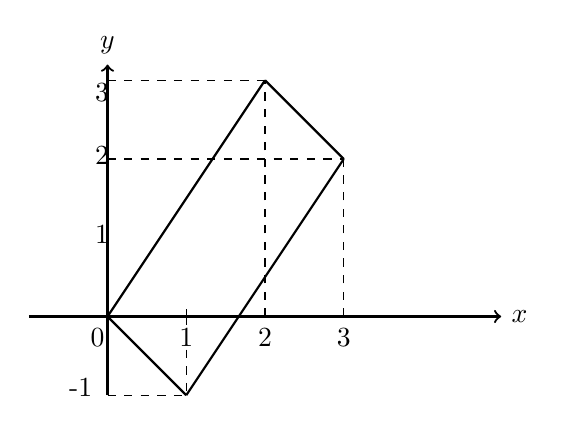
\begin{tikzpicture}
\draw[->,thick] (-1,0) -- (5,0) node[right,scale=1]{$x$};
\draw[->,thick] (0,-1) -- (0,3.2) node[above,scale=1]{$y$}; 
\draw[thick] (0,0) -- (2,3);
\draw[thick] (0,0) -- (1,-1);
\draw[thick] (1,-1) -- (3,2);
\draw[thick] (3,2) -- (2,3);
\draw[dashed] (3,0) -- (3,2);
\draw[dashed] (2,0) -- (2,3);
\draw[dashed] (0,2) -- (3,2);
\draw[dashed] (0,3) -- (2,3);
\draw[dashed] (1,0) -- (1,-1);
\draw[dashed] (0,-1) -- (1,-1);
\draw (0,0) -- (0,0.1) node[left=3.6,below=3.6pt]{0};
\draw (1,0) --(1,0.1) node[below=3.6pt]{1};
\draw (0,1) --(0,1.3) node[left=2,below=0.6pt]{1};
\draw (0,-1) --(0,-0.9) node[left=2]{-1};
\draw (2,0) --(2,0.1) node[below=3.6pt]{2};
\draw (3,0) --(3,0.1) node[below=3.6pt]{3};
\draw (0,3) --(0,3.1) node[left=2,below=0.6pt]{3};
\draw (0,2) --(0,2.3) node[left=2,below=0.6pt]{2};
%\draw (0,0) circle [radius=1.5cm]; 
\end{tikzpicture}

$$\left(\begin{array}{l}
x\\
y
\end{array}\right)=\left(\begin{array}{cc}
1&2\\
-1&3
\end{array}\right)\left(\begin{array}{l}
u\\
v
\end{array}\right)$$

$\therefore$ $\left\{\begin{array}{ll}
x=u+2v& dx=du+2dv\\
y=-u+3v & dy=-du+3dv 
\end{array}\right.$\\

$\begin{aligned}
S(\Delta)&=\iint_\Delta dxdy\\
&=\iint_\Delta(du+2dv)\land(-du+3dv)\\
&=\iint_\Delta(3+2)du\land dv\\
&=5\iint_\Delta dudv=5
\end{aligned}$\hspace{2cm}
$\begin{array}{l}
du\land du=-du\land du\\
\Rightarrow du\land du=0
\end{array}$\\
另一种方法求面积\\
$\left|\left|\begin{array}{cc}
1&2\\
-1&3
\end{array}\right|\right|=|5|=5$\hspace{2cm}
$J=\left|\frac{\partial(x,y)}{\partial(u,v)}\right|=\left|\begin{array}{cc}
1&2\\
-1&3
\end{array}\right|=5$\\
\begin{center}
	$\begin{aligned}
	-\iint_\Delta dxdy=\iint_DJdudv=5\iint_Ddudv=5.
	\end{aligned}$
\end{center}


\noindent 例2.计算区域$D, 0\leq r\leq1, 0\leq\theta\leq2\pi$的面积。\\
\begin{tikzpicture} 
%\draw[step=1,color=gray!40] (-2,-2) grid (2,2); 
\draw[->] (-2,0) -- (2,0) node[right=1.6pt]{x}; 
\draw[->] (0,-2) -- (0,2) node[right=1.6pt]{y}; 
\draw (1,0) --(1,0.1) node[right=1.6pt,below=1.6pt]{1};
\draw (0,0) circle (1);  
\end{tikzpicture} 
\qquad\qquad\qquad
\begin{tikzpicture}
\draw[->,thick] (-1,0) -- (2,0) node[right,scale=1]{$r$};
\draw[->,thick] (0,-1) -- (0,3) node[right,scale=1]{$\theta$}; 
\draw[thick] (1,0) -- (1,1.5);
\draw[thick] (0,1.5) -- (1,1.5);
\draw (0,0) -- (0,0.1) node[left=3.6,below=3.6pt]{0};
\draw (1,0) --(1,0.1) node[below=3.6pt]{1};
\draw (0,1.5) --(0,1.8) node[left=6,below=0.6pt]{$2\pi$};
%\draw (0,0) circle [radius=1.5cm]; 
\end{tikzpicture}

\qquad$D:x^{2}+y^{2}\leq 1$\qquad\qquad\qquad\qquad $\Delta:0\leq r\leq 1,0\leq \theta\leq 2\pi$ \\
解:进行坐标变换$\left\{\begin{array}{ll}
x=r\cos\theta&0\leq\theta\leq2\pi\\
y=r\sin\theta&0\leq r\leq1
\end{array}\right.$
,于是
\[\begin{split}
&S(\Delta)=\iint_\Delta dxdy=\iint_D d(r\cos\theta)\land d(r\sin\theta)\\
&=\iint_D(\cos\theta dr-r\sin\theta d\theta)\land(\sin\theta dr+r\cos\theta d\theta)\\
&=\iint_D r\cos\theta^2 drd\theta-r\sin^2\theta d\theta dr\\
&=\iint_D r(\cos\theta^2+\sin^2\theta)drd\theta\\
&=\iint_D rdrd\theta\\
&=\int_{0}^{2\pi}d\theta\int_{0}^{1}rdr=2\pi\cdot\frac{1}{2}=\pi
\end{split}
\]

一般地,设$D$是$\mathbb{R}^{n}$中区域,$x_{1},x_{2},\cdots,x_{n}$是$D$上坐标,进行坐标变换
$\left(\begin{array}{l}
y_{1}\\
\vdots\\
y_n
\end{array}\right)=A\left(\begin{array}{l}
x_{1}\\
\vdots\\
x_n
\end{array}\right)$
$A\in M_n(\mathbb{R}), y_i=a_{i1}x_1+\cdots+a_{in}x_n, (1\leq i\leq n)$,得到$\mathbb{R}^{n}$中区域$D^{'}$,则
\begin{center}
	$\begin{aligned}
	vol(D^{\prime})&=\int\cdots\int_{D^{'}} dy_1\land\cdots\land dy_n\\
	&=\int\cdots\int_D d(a_{11}x_1+\cdots a_{1n}x_n)\land\cdots\land d(a_{n1}x_1+\cdots+a_{nn}x_n)\\
	&=|A|\int\cdots\int_Ddx_1\land dx_2\land\cdots\land dx_n
	\end{aligned}$
\end{center}
$|A|=J=\left|\frac{\partial(y_1\cdots y_n)}{\partial(x_1\cdots x_n)}\right|.$\\

\subsection{分式模}

$A$环(交换环)\\
$S$是$A$的乘法封闭子集$S\subset A$,
$$S^{-1}A=\left\{\frac{a}{s}|a\in A, s\in S\right\}.$$
设$M\in A-Mod$,分式模为
$$S^{-1}M=\left\{\frac{x}{s}|x\in M, s\in S^\prime\right\}.$$
$\frac{x_1}{s_1}=\frac{x_2}{s_2}\Leftrightarrow \exists t\in S$使得$t(s_2x_1-s_1x_2)=0.$\\
有自然映射

$$
A\rightarrow S^{-1} A$$
$$
a\mapsto \frac{a}{1}
$$
这样$S^{-1}A$可看成一个$A-Mod$.\\
%设有环同态$f:A\rightarrow B,$
%S^{-1}A\bigotimes_AM\simeq S^{-1}M\quad (A\text{模同构})\\
%定义$a\cdot b\stackrel{\Delta}{=}f(a)\cdot %b.&\left(\frac{a}{s}, m\right)\mapsto\frac{am}{s}$
由定义,$\frac{x_1}{s_1}\sim\frac{x_2}{s_2}(x_1,x_2\in M, s_1, s_2\in S^{-1}\Leftrightarrow \exists t\in S$使得$t(s_2x_1-s_1x_2)=0$。
易知``$\sim$"是$S\times M$中的一个等价关系.
$\frac{x}{s}$即为$(s,x)\in S\times M$关于``$\sim$"的等价类.\\
定义$S^{-1}M$中加法为
\noindent ``+": $\frac{x_1}{s_1}+\frac{x_2}{s_2}\stackrel{\Delta}{=}\frac{s_2x_1+s_1x_2}{s_1s_2}.$\\
数乘($S^{-1}A$对$S^{-1}M$的作用):
\begin{center}
	$\begin{array}{l}
	S^{-1}A\times S^{-1}M\rightarrow S^{-1}M\\
	\left(\frac{a}{s},\frac{x}{t}\right)\mapsto \frac{a}{s}\frac{x}{t}\stackrel{\Delta}{=}\frac{ax}{st}\quad(\forall a\in A, s,t\in S, x\in M)
	\end{array}$
\end{center}
$\therefore S^{-1}M\in S^{-1}A-Mod$.\\
即上述构造所得$S^{-1}M$是一个$S^{-1}A$-模,称为$M$关于$S$的\textbf{分式模}。\\
事实:设$A,B$是交换环,$f:A\rightarrow B$是一个环同态\\
则:$\begin{array}{l}
A\times B\rightarrow B\\
(a,b)\mapsto a\star b
\end{array}$(注:若$A,B$是非交换环,则$f(A)\subset C(B)$)\\
其中$a\star b\stackrel{\Delta}{=}f(a)\cdot b$.
于是易验证$(B,+,\star)$是一个$A-$模,此时也称$B$为一个$A-$代数.\\
若$B$与$C$为$A-$代数,则可定义\\
\begin{center}
	$\begin{array}{l}
	B\bigotimes_AC\\
	(b_1\bigotimes c_1)(b_2 \bigotimes c_2)=(b_1b_2)\bigotimes(c_1c_2)\\
	\Rightarrow B\bigotimes_AC\text{也是一个}A-\text{代数.}
	\end{array}$
\end{center}

\begin{itemize}
	\item[定理:] 设$A$是含1交换环,$S$是$A$的一个乘法封闭子集,$M\in A-Mod$,则
	$$
	S^{-1}A\otimes_{A}M\cong S^{-1}M.
	$$
	\item[证明:] 首先,令$$
	f:S^{-1}A\times M\rightarrow S^{-1}M$$
	$$
	\left(\frac{a}{s},x\right)\mapsto \frac{ax}{s}\in M. 
	$$
	$\because M\in A-Mod,f(\frac{a}{s},x_1)\stackrel{\Delta}{=}\frac{ax}{s}(\forall\frac{a}{s}\in S^{-1}A, x\in M).$
	易验证,$f$是$A-$双线性映射,从而由张量积的泛性质:
	$\exists!$的$A-$线性映射$\phi=S^{-1}A\otimes_AM\rightarrow S^{-1}M$,
	使得$f=\phi\circ\eta$,即下图交换
	$$
	\xymatrix{
		S^{-1}A\times M\ar[rr]^{\eta}\ar[rd]_{f}& &S^{-1}A\otimes_{A}M\ar[ld]^{\phi}\\
		&S^{-1}M&
	}
	$$
	
	$$
	\phi:S^{-1}A\otimes_AM\rightarrow S^{-1}M$$
	$$
	\frac{a}{s}\otimes_{A}x\mapsto\frac{ax}{s}
	$$	
\end{itemize}
\noindent 下证$\phi$是一个同构。


由于$\forall s\in S, x\in M$,有$\frac{x}{s}=f(\frac{1}{s}\otimes x)$,从而$\phi$是满射。


下证$\phi$是一个单射。为此,任取$\alpha\in S^{-1}M$有$\alpha=\sum_{i=1}^{n}\frac{a_i}{s_i}\otimes x_i$,其中$a_i\in A, s_i\in S, x_i\in M, (i-1,\cdots,n)$。
令$s=s_1\cdots s_n$, $s^\prime=\frac{s}{s_i}$,
\begin{center}
	$\begin{aligned}
	\alpha=\sum_{i=1}^{n}\frac{a_i}{s_i}\otimes x_i&=\sum_{i=1}^{n}\frac{a_is^\prime}{s}\otimes x_i=\sum_{i=1}^{n}\frac{1}{s}\times (a_is^\prime x_i)\\
	&=\frac{1}{s}\sum_{i=1}^{n}1\otimes(a_is^\prime x_i)\\
	&=\frac{1}{s}\left(1\otimes\sum_{i=1}^{n}(a_is^\prime x_i)\right)\\
	&=\frac{1}{s}(1\otimes x)\qquad\text{其中}x=\sum_{i=1}^{n}a_is^\prime x_i\\
	&=\frac{1}{s}\otimes x.
	\end{aligned}$
\end{center}

\begin{center}
	$\begin{aligned}
	\therefore\alpha=\frac{1}{s}\otimes x\in Ker\theta&\Leftrightarrow0=\phi(\alpha)=\phi(\frac{1}{s}\otimes x)=\frac{x}{s}=0\\
	&\Leftrightarrow \exists t\in S, \text{使得}t(x\cdot1-s\cdot0)=tx=0
	\end{aligned}$
\end{center}
故
\begin{center}
	$\begin{aligned}
	\alpha&=\frac{1}{s}\otimes x=\frac{t}{st}\otimes x\\
	&=\frac{1}{st}\otimes tx=\frac{1}{st}\otimes0=0\\
	\end{aligned}$
\end{center}
$\Rightarrow ker\phi=0$$\therefore \phi$是单的。
从而$\phi$呈同构。\\
上述构造所得$S^{-1}M$是一个$S^{-1}A$-模,称为$M$关于$S$的分式模.\\

\noindent Jordan-Holder定理

设$M\in A-$mod, 如果有序列
$$M=M_0\subsetneqq M_1\subsetneqq M_2\cdots\subsetneqq M_n=0(\star)$$
其中$M_i\leq M(i=0,1,2\cdots n)$,
且$M_i/M_{i+1}$均是单$-A$模($i=0,1,\cdots,n-1$),
则称$(\star)$为一个合成列(comprosition serise).
$M_i/M_{i+1}$称为$M$的合成因子,其中$n$标为$M$的长度(length)记为$l(M)=n$.


\textbf{定理(Jordan-Holder)} 设$M\in A-Mod$,如果$M$有合成列,则$M$的所有$h$合成列都有相同的长度,且他们的合成因子在相差一个置换下的对应互相同构。把合成因子$M_{i}/M_{i+1}$作直和$M^{'}=\bigoplus\limits_{i=1}^nM_{i}/M_{i+1}$,当$M$不是半单时,可由$M^{'}$去找合成列。

\section{域论}

\subsection{域的代数扩张}

域$F,(F,+,\cdot),u(F)=F^{*}=F/{0}$,子域$F_{i}\leqslant F$其中$i\in I$,$\cap F_{i}\leqslant F.$


证明:由于$0,1 \in F_{i}, \forall i\in I, \Rightarrow 0,1\in \bigcap\limits_{i\in I}F_i$.

\hspace{11pt}而$\forall a, b \in F_{i}, i\in I, \Rightarrow a+b\in F_i, \forall i\in I\Rightarrow a+b\in\bigcap\limits_{i\in I}F_i$

\hspace{148pt}$ab\in F_i, \forall i\in I\Rightarrow ab\in\bigcap\limits_{i\in I}F_i$

\hspace{27pt} $\bigcap\limits_{i\in I}F_i\leqslant F$是$F$的子域。

$\alpha\in F,$则$\alpha^{2},\alpha^{3} \ldots \alpha^{n} \in F\ (\forall n\in N)$, $a_{0} \cdot 1+a_{1} \cdot \alpha+1+a_{n} \alpha^{n} \in F.$
令$f(\alpha)=a_{0}+a_{1} \alpha+\cdots+a_{n} \alpha^{n} \in F$,即$\alpha\in F, f(\alpha)\in F$.

若$g(x)\in F[x], g(\alpha)\neq 0$,则$\dfrac{f(\alpha)}{g(\alpha)} \in F$
%记$h=\dfrac{f}{g}\in F(x)$,

$F$是域,$F$上的关于$x$的多项式环$F[x]$,
$F$上的关于$x$的有理分式域$F(x)$,如$\mathbb{R}(x)$,$\mathbb{C}(x)$

一般地,$F$上关于$x_{1} \cdots x_{n}$的多项式环为$F[x_{1} \cdots x_{n}]$;$F$上关于$x_{1} \cdots x_{n}$的有理分式域$F(x_{1} \cdots x_{n}).$\\

固定一个域$k$,任取$k$的一个子域$F$,任取$\alpha\in k$.
问题:$k$中包含$F$与$\alpha$的最小子域是?

答案:$F(\alpha)=\{h(\alpha) \mid h \in F(x) \mid h(\alpha)\text{  有意义 }\}=\left\{ \left.\dfrac{f(\alpha)}{g(\alpha)}\right| f,g\in F[x]\text{ 且 }\ g(\alpha)\neq 0\right\}$

\hspace{11pt}$F(\alpha) \triangleq\bigcap\limits_{E\in k\atop E\supset FU(\alpha)}E$,称$F(\alpha)$为$F$添加$k$中元$\alpha$生成的子域。

同理,
$$
\begin{aligned}
F\left( \alpha_1,\alpha_2\right)&=\left\{ h\left(\alpha_{1}, \alpha_{2}\right) \mid h \in F\left(x_{1}, x_{2}\right), h\left(\alpha_{1}, \alpha_{2}\right)\text{ 有意义 }\right\}\\ 
&=\left\{ \dfrac{f(\alpha_1, \alpha_2)}{g(\alpha_1, \alpha_2)}\mid f, g \in F\left[x_{1}, x_{2}\right]\text{ 且 }\ g(\alpha_1, \alpha_2) \neq 0\right\}
\end{aligned}
$$

对于$\alpha_{1} \cdots \alpha_{n} \in k$
$$
F\left( \alpha_{1} \cdots \alpha_{n}\right)=\left\{ \left.\dfrac{f\left( \alpha_{1} \cdots \alpha_{n}\right)}{g\left( \alpha_{1} \cdots \alpha_{n}\right)}\right| f,g\in F\left[ x_{1} \cdots x_{n}\right]\text{ 且 }\ g\left( \alpha_{1} \cdots \alpha_{n}\right)\neq 0\right\}
$$

设$F\leqslant k$子域,$S^{\prime}\subset k$子集,$S\neq\varnothing$,$F(S)$为$k$中既包含$F$又包含$S^{\prime}$的最小子域,
$$
F(S)=\left\{ \left. \dfrac{f\left( \alpha_{1} \cdots \alpha_{n}\right)}{g\left( \alpha_{1} \cdots \alpha_{n}\right)}\right| n\in N, \alpha_{1} \cdots \alpha_{n}\in S, f,g\in F\left[\alpha_{1} \cdots \alpha_{n}\right], g\left( \alpha_{1} \cdots \alpha_{n}\right)\neq 0\right\}
$$
每个元素都可只加$S$中的有限个元即可得到。\\


固定$k$域,$F_1,F_{2} \leq k$是$k$的两个子域.
问:$k$中既包含$F_1$又包含$F_2$的最小子域是?

答:$F_{1}\left(F_{2}\right)=F_{2}\left(F_{1}\right)\triangleq F_1F_2$称之为$F_1$与$F_2$的合成(域)。

类似地,对于$k$的子域$F_i\ (i=1,\cdots, n)$,$F_i$的合成记为$F_1\cdots F_n$代数扩张。

域扩张:设$F, k$是域,如果$F\subset k$,则知$F$为$k$的子域,$k$是$F$的一个扩域,则$k$可作为$F$模$\Rightarrow k$ 可作为$F$向量空间。

此时,$k$是$F$上一个向量空间,$F \times k \longrightarrow k$,$(a, b) \longmapsto a b$

\textbf{定义}:设$k/F$是一个域扩张$(F\subset k)$,称$\operatorname{dim}_F^k$为其扩张次数,记之为$\left[ k: F\right]\triangleq\operatorname{dim}_F^k$

\hspace{11pt}当$\left[ k: F\right]=n<+\infty$时,称$k/F$为一个$n$次扩张。

\hspace{11pt}当$\left[ k: F\right]=+\infty$时,称$k/F$为一个无限扩张。

\textbf{定义}: 设$k/F$是一个域扩张,$\alpha\in k$,如果有$f(x)\in F[x] \mid\{ 0\}$,使得$f(\alpha)=0$,则称$\alpha$在$F$上代数,也称$\alpha$是一个$F$代数元。

若这样的非零多项式不存在,则称$\alpha$是$F$上的数据元。

此时,$f(x)=a_n x^{n}+a_{n-1} x^{n-1}+\cdots+a_{1} x+a_{0}\in F[x] \mid \{ 0\}$,$a_0,\cdots, a_n\in F$,$n=\operatorname{deg}f, a_n\neq 0$,且显然$n>0$。

\textbf{定义}:设$k/F$是一个域扩张,如果$k$中任一元素均是下一代数元,则称$k/F$是一个代数扩张。

\textbf{定理1}:域的有限扩张均是代数扩张,即对于域扩张$k/F$,如果$[k: F]<+\infty$,则$k/F$是一个代数扩张。

证明:设$[k: F]=n<+\infty, \forall\alpha\in k$(只需证$\alpha$是$F$一代数元即可)

\hspace{11pt}则$1,\alpha_1,\cdots,\alpha_n$是$F$一线性相关的($\because\operatorname{dim}_F^k=n$)

\hspace{11pt}$\therefore$存在不全为0的$a_0\cdots a_n\in F$,使得
$$
a_{0}+a_{1} \alpha+\cdots+a_n\alpha^{n}=0
$$

\hspace{11pt}令$f(x)=1+a_{1} x+\cdots+a_{n} x^{n}  \in  F[x] \mid \{0 \}$,且$f(\alpha)=0$

\hspace{11pt}$\therefore\alpha$是$F$一代微元,

\hspace{11pt}$\therefore k/F$是代数扩张。\hfill$\Box$

\textbf{定理2:}设域$F\subset E\subset k$,如果$E/F$,$k/E$都是有限扩张,则$k/F$是有限扩张,且$[k: F]=[k: E][E: F]$

证明:设$[E: F]=m, [k: E]=n$,则$\operatorname{dim}_F^F=m$,$\operatorname{dim}_E^k=n.$
取$\left\{x_{1}, \cdots, x_{m}\right\}$是$E$上的一组$F$-基;
$\left\{y_{1}, \cdots, y_{n}\right\}$是$k$上的一组$E$-基.


下证$\left\{ x_iy_j\right\}_{1\leqslant i\leqslant m\atop 1\leqslant j\leqslant n}$是$k$的一组$F$-基.

$\forall\alpha\in k$,有$\alpha=\sum\limits_{j=1}^{n} x_{j} y_{j}$,其中$b_j\in E$,而$\forall b_j\in E$,有$b_j=\sum\limits_{i=1}^{m} a_{ij}x_i$,其中$a_{ij}\in F$
\begin{center}
	
	$\begin{aligned} \Rightarrow\alpha=\sum\limits_{j=1}^{n} b_{j} y_{j} &=\sum\limits_{j=1}^{n}\left(\sum\limits_{i=1}^{m} a_{i j} x_{i}\right) y_{j} \\ &=\sum\limits_{j=1}^{n} \sum\limits_{i=1}^{m} a_{i j} x_{i} y_{j} .\end{aligned}$
\end{center}
$\therefore k$中任一元素都可用$\left\{ x_iy_j\right\}_{1\leqslant i\leqslant m\atop 1\leqslant j\leqslant n}$ $F$-线性表出

设
$$\sum\limits_{i=1}^{m} \sum\limits_{j=1}^{n} a_{i j} x_{i}  y_{j}=0, a_{ij}\in F,$$
则
$$\sum\limits_{j=1}^{n}\left(\sum\limits_{i=1}^{m} a_{ij} x_{i}\right) y_{j}=0.$$
由于$\sum\limits_{i=1}^ma_{ij}^{\in F}x_i^{\in E}\in E$,由$\left\{ y_1,\cdots,y_n\right\}$线性无关
$\Rightarrow\sum\limits_{i=1}^{m} a_{ij} x_{i}=0(\forall j)$,由于$a_{ij}\in F$,$\left\{ y=x_1,\cdots,x_m\right\}$\\是$E$上关于$F$的一组基$\Rightarrow a_{ij=0}$,于是$a_{ij=0}(i=1,\cdots, m, 1\leqslant j\leqslant n)$.

从而$\left\{ x_iy_j\right\}_{1\leqslant i\leqslant m\atop 1\leqslant j\leqslant n}$是一组$k$的$F$-基.
且有$[k: F]=[k: E][E: F]=mn.$\hfill$\Box$

同理设域扩张$F=F_0\subset F_1\subset \cdots \subset F_n$,则
$$
[F_n: F]=[F_n: F_{n-1}][F_{n-1}: F_{n-2}]\cdots [F_1: F]
$$

\textbf{定理}:(单代数扩张结构定理)设$k/F$是一个域扩张,$\alpha\in k$且$\alpha$是$F$-代数元,则$F(\alpha)=F[\alpha]$\\且$[F(\alpha): F]=n<+\infty$。特别地,$F(\alpha)/F$是代数扩张,其中$n$为$\alpha$在$F$上极小多项式的次数。

\subsection{代数扩张与单代数扩张结构}

域的特征:$F$域,有整数环到$F$的自然嵌入
\[
\begin{split}
\phi:&\mathbb{Z} \rightarrow F\\
1 &\mapsto 1_{F}
\end{split}
\]
则ker $\phi=<n>,\ n\in\mathbb{Z}\geqslant 0$.于是
$Z/\text{ker }\phi\hookrightarrow F$子域$\Rightarrow\text{ ker}\phi$ 是$\mathbb{Z}$中极大理想,或0。

域$F$的特征,若$\text{ch}(F)=0,$则$ \mathbb{Z}\subset F$,又域有逆元,$\mathbb{Q}\subset F$,即$\mathbb{Q}$是$F$的最小子域(或称素子域)

若$\text{ch}(F)=p$(素数),此时$F_p=\mathbb{Z}/p\mathbb{Z}\subset F$,即$F_p$为$F$的素子域。

\textbf{定理1}:(域的单代数扩张结构):设$k/F$是一个域扩张,$\alpha\in k$,记$E=F(\alpha)$
\begin{enumerate}
	\item[(1)] 存在$F$上唯一一个首 1 不可约多项式$P_{\alpha}(x)\in F[x]$,使得$P_{\alpha}(x)=0$,记$n=\operatorname{deg}P_{\alpha}(x)$
	\item[(2)] $E=F(\alpha)=F[x]$且$\{ 1,\alpha,\alpha^2,\cdots,\alpha^{n-1}\}$是$E$的一组$F$-基,特别地,$[F(\alpha): F]=\operatorname{deg}P_{\alpha}(x)$,称上述$P_{\alpha}(x)$为$\alpha$在$F$上的极小多项式(书上记之为$P_{\alpha}(x)=I_{rr}\left( \alpha, F, x\right)$)
\end{enumerate}

先给出一个引理及证明,利用引理去证明定理 1。

引理:设$\alpha$,$k/F$如上述定理,记$I=\left\{ f(x)\in F[x] \mid f(\alpha)=0\right\}$,则$I=\langle P_{\alpha}(x)\rangle$是一个素理想,其中$P_{\alpha}(x)\in F[x]$是$F$上一个首 1 的不可约多项式。

证明:令
\[\begin{split}
\phi:F[x]&\longmapsto k\\
f(x)&\longmapsto f(\alpha)
\end{split}
\]

\quad 则$\phi$是环同态,且$\text{ker}\phi=\left\{ f\in F[x] \mid f(\alpha)=0\right\}=I$

\quad 于是由环同态基本定理,有
$$
F[x]/I\backsimeq Im(\phi)\leqslant k\text{ 子环}
$$

\quad 因为$k$是域,故$F[x]/I$是整环$\Rightarrow\ I$是素理想。

\quad 又$F[x]$是一个PID,由于$\alpha$是$F$-代数元,故$\exists\ f\in F[x] - \{ 0\}$,使得$f(\alpha)=0$,即$I\neq 0\Rightarrow\ I$是极大理想。

\quad 从而$I$是由一个不可约多项式生成(把首项系数化为 1,得到的理想也相同)记为$P_{\alpha}(x)$,即$I=\langle P_{\alpha}(x)\rangle$\hfill$\Box$

证明定理:

(1)由上述引理即得

(2)设$P_{\alpha}(x)$为(1)中所给的$\alpha$在$F$上的极小多项式,$n=\operatorname{deg}P_{\alpha}(x)$,于是可设$P_{\alpha}(x)=x^n+a_{n-1}x^{n-1}+\cdots +a_1x+a_0\in F[x]$


下证$F(x)=F[\alpha]$.

为此,任取$\beta\in F(\alpha)$,则$\beta=\dfrac{f(\alpha)}{g(\alpha)}, f,g\in F[x]$,且$g(\alpha)\neq 0$.
由极小多项式的性质,$P_{\alpha}(x)\nmid g(x)$.
又$P_{\alpha}(x)$不可约,则$\left( P_{\alpha}(x), g(x)\right)=1$,又$F[x]$是PID,
$\therefore$有$u(x), v(x)\in F[x]$,使得
$$
u(x)P_{\alpha}(x)+v(x)g(x)=1
$$
\[
\begin{split}
&\Rightarrow u(\alpha)P_{\alpha}(\alpha)+v(\alpha)g(\alpha)=1\\
&\Rightarrow v(\alpha)g(\alpha)=1\\
& \Rightarrow\dfrac{1}{g(\alpha)}=u(\alpha)\\
& \Rightarrow\beta=\dfrac{f(\alpha)}{g(\alpha)}=f(\alpha)\cdot v(\alpha)\in F[\alpha]\\
& \Rightarrow F(\alpha)\subset F[\alpha]\\
\end{split}
\]
\quad 显然$\Rightarrow F(\alpha)\supset  F[\alpha]$
$\Rightarrow F(\alpha)=F[\alpha]$.

\quad

下证$\left\{ 1,\alpha,\cdots, \alpha^{n-1}\right\}$是$E$的一组$F$-基.

由带余除法有$f(x)=g(x)P_{\alpha}(x)+r(x)$,其中$g(x)\cdot r(x)\in F[x]$,且$r(x)=0$或$\operatorname{deg}r(x)<\operatorname{deg}P_{\alpha}(x)=n$

于是
$$
\beta=f(\alpha)=gf(\alpha)P_{\alpha}(\alpha)+r(\alpha)=r(\alpha)\in F+F\alpha+\cdots +F\alpha^{n-1}
$$
即$\beta$可由$\left\{ 1,\alpha,\cdots, \alpha^{n-1}\right\}$的$F$-线性表述。

下证$\left\{ 1,\alpha,\cdots, \alpha^{n-1}\right\}$线性无关。

设$b_0+b_1\alpha+\cdots +b_{n-1}\alpha^{n-1}=0$,其中$b_0,\cdots,b_{n-1}\in F$.
令$g(x)=b_0+b_1x+\cdots +b_{n-1}x^{n-1}\in F[x]$,
则$g(\alpha)=0$,从而$P_{\alpha}(x) \mid g(x)$.
由于$\operatorname{deg}g(x)=n-1<\operatorname{deg}P_{\alpha}(x)$

$$\Rightarrow g(x)=0\Rightarrow b_0=b_1=\cdots=b_{n-1}=0,$$
从而$\left\{ 1,\alpha,\cdots, \alpha^{n-1}\right\}$是线性无关的。

综上,$\left\{ 1,\alpha,\cdots, \alpha^{n-1}\right\}$是$E$的一组$F$-基。\hfill$\Box$\\


\textbf{定义}:设$k/F$是一个域扩张,如果有$\alpha_1,\cdots,\alpha_n\in k$,使得$k=F\left( \alpha_1,\cdots,\alpha_n\right)$,则称$k$是$F$的一个有限生成扩域,或称$k/F$是一个有限生成扩张。

证明:“$\Longleftarrow$”\quad $k=F\left( \alpha_1,\cdots,\alpha_n\right)=F\left[ \alpha_1,\cdots,\alpha_n\right]$,其中$\alpha_1,\cdots,\alpha_n\in k$都是$F$-代数元

$$k=F\left[ \alpha_1,\cdots,\alpha_{n-1}\right]\left[ \alpha_n\right],F\left[ \alpha_1,\cdots,\alpha_{n-1}\right]=F\left[ \alpha_1,\cdots,\alpha_{n-2}\right]\left[ \alpha_{n-1}\right]$$
$$\cdots$$
\[
\begin{split}
\Rightarrow\ \left[ k: F\right]&=\left[ k: F\left[ \alpha_1,\cdots,\alpha_{n-1}\right]\right]\\
&=\left[ F\left[ \alpha_1,\cdots,\alpha_{n-1}\right]: F\left[ \alpha_1,\cdots,\alpha_{n-2}\right]\right]\cdots\left[ F\left[ \alpha_2,\alpha_1\right]: F\left[ \alpha_1\right]\right]\\
&<+\infty.
\end{split}
\]

“$\Longrightarrow$”\quad 由于$[k: F]=n<+\infty$,故$k$作为$F$的向量空间有一组基.
设$\alpha_1,\cdots,\alpha_n$为$k$的一组$F$-基

于是
$$k=F\alpha_1+F\alpha_2+\cdots+F\alpha_n\subset F\left[ \alpha_1,\cdots,\alpha_n\right]\subset k(\Leftarrow \because \alpha_1,\cdots,\alpha_n\in k, F\subset k)$$

即$k=F\left[ \alpha_1,\cdots,\alpha_n\right]$.
从而$k$是$F$上一个有限生成的代数扩张。\hfill$\Box$\\


例1:\ $F=Q\left( \sqrt[3]{2}\right)=Q\left( \sqrt[3]{2}\right),\quad \alpha=\dfrac{1}{2-\sqrt[3]{2}+\sqrt[3]{4}}\in F$,找$f(x)\in Q[x]$,使得$\alpha=f\left( \sqrt[3]{2}\right)$

解:\quad\ $\sqrt[3]{2}$在$Q$中的极小多项式为$P(x)=x^3-2$,不可约的

\quad 而令$g(x)=x^2-x+2$,则$g\left( \sqrt[3]{2}\right)=\sqrt[3]{4}-\sqrt[3]{2}+2$,即$\alpha=\dfrac{1}{g\left( \sqrt[3]{2}\right)}$

\quad 对$P(x)$与$g(x)$作辗转粗除法
$$
\begin{aligned}
P(x)&=x^{3}-2=(x+1)\left(x^{2}-x+2\right)-x-4\\ 
g(x)&=(-x-4)(-x+5)+22\\ 
\Rightarrow 22&=g(x)+(x+4)(-x+5)\\ 
&=g(x)+[(x+1) g(x)-P(x)](-x+5)\\ 
&=g(x)+\left(-x^{2}+4 x+5\right) g(x)-P(x)(-x+5)\\
&=\left(-x^{2}+4 x+6\right) g(x)-P(x)(-x+5)\\ 
\Rightarrow 22&=\left(-\sqrt[3]{4}+4\sqrt[3]{2}+6\right) g(\sqrt[3]{2})-P(\sqrt[3]{2})(-\sqrt[3]{2}+5)\\ 
&=\left(-\sqrt[3]{4}+4\sqrt[3]{2}+6\right) g(\sqrt[3]{2})\\ 
\Rightarrow\alpha&=\dfrac{1}{g\left(\sqrt[3]{2}\right)}=\dfrac{1}{22}\left(-\sqrt[3]{4}+4\sqrt[3]{2}+6\right)
\end{aligned}
$$

\quad $\therefore$取$f(x)=\dfrac{1}{22}\left(-x^{2}+4 x+6\right)$即可得到$\alpha=f\left(\sqrt[3]{2}\right)$\hfill$\Box$

\quad

\noindent
\hangafter=1
\setlength{\hangindent}{3em}
命题:设有域扩张$F\subset E\subset k$,则$k/F$是代数扩张$\Longleftrightarrow\ E/F,\ k/E$都是代数扩张。

证明:“$\Longrightarrow$”\quad 若$k/F$是代数扩张,则$\forall\ \alpha\in k$,$\alpha$在$F$上代数,则自然在$E$上也代数,$\therefore\ k/E$是代数扩张。由于$\forall\ \alpha\in E$,自然$\alpha\in k$,由于$k/F$是代数扩张,则$\alpha$在$F$上的代数元,则$E/F$是代数扩张。

$\Longleftarrow$”\quad 任取$\alpha\in k$,下证$\alpha$是$F$-代数元。

由于$k/E$是代数扩张,则$\alpha$是$E$-代数元,则有
$$
f(x)=a_{n} x^{n}+a_{n-1} x^{n-1}+\cdots+a_{1} x+a_{0}\in E[x] \mid \{ 0\}
$$
使得$f(\alpha)=0$。

令
$$E_1=F\left[ a_0,\cdots,a_n\right]=F\left( a_0,\cdots,a_n\right),$$
则$f(x)\in E_1[x]$且$\alpha$在$E_1$代数。 
由于$a_0,\cdots,a_n\in E$,又$E/F$是代数扩张,则$a_0,\cdots,a_n$在$F$上代数。 
则$E_1=F\left[ a_0,\cdots,a_n\right]/F$是一个有限扩张.

综上,$\left[ E_1\left( \alpha\right): F\right]=\left[ E_1\left( \alpha\right): E_1\right]\left[ E_1: F\right]<+\infty$.
从而$E_1\left( \alpha\right)/F$是代数扩张 .

$\therefore\ \alpha$在$F$上代数,由$\alpha$的任一性,
$\Rightarrow\ k/F$是代数扩张 .

\subsection{代数闭包(1)}

$\begin{array}{cccc}
\alpha &\in &k &\text{ 域扩张 }\\ 
&&\mid &\\ 
&&F &
\end{array}$\qquad $f(x)\in F[x]$,使得$f(\alpha)=0$,
$\tau|F=\sigma$ \\ 
$\tau$为$\sigma$延拓\\ 
$\sigma$为$\tau$在$F$上的限制

设$f(x)=x^{n}+a_{n-1} x^{n-1}+\cdots+a_{1} x+a_{0}\in F[x]$,\ $0=f(\alpha)=\alpha^{n}+a_{n-1}\alpha^{n-1}+\cdots +a_{1}\alpha+a_{0}$
$$
\begin{aligned}
0=\tau\left( 0\right)=\tau\left( f\left( \alpha\right)\right)&=\tau\left( \alpha^{n}+a_{n-1}\alpha^{n-1}+\cdots+a_{1}\alpha+a_{0}\right)\\ 
&=\tau\left( \alpha\right)^n+\tau\left( a_{n-1}\right)\tau\left( \alpha\right)^{n-1}+\cdots+\tau\left( a_1\right)\tau\left( \alpha\right)+\tau\left( a_0\right)\\ 
&=\tau\left( \alpha\right)^n+\sigma\left( a_{n-1}\right)\tau\left( \alpha\right)^{n-1}+\cdots+\sigma\left( a_1\right)\tau\left( \alpha\right)+\sigma\left( a_0\right)
\end{aligned}
$$

即$$\tau\left( \alpha\right)^n+\sigma\left( a_{n-1}\right)\tau\left( \alpha\right)^{n-1}+\cdots+\sigma\left( a_1\right)\tau\left( \alpha\right)+\sigma\left( a_0\right)=0.$$

令$$g(x)=x^{n}+\sigma\left(a_{n-1}\right) x^{n-1}+\cdots+\sigma\left(a_{1}\right) x+\sigma\left(a_{0}\right),$$

即$g\left( \tau\left( \alpha\right)\right)=0$,即$\tau\left( \alpha\right)$是$g\left( x\right)$的一个根.
常记$g(x) \triangleq f^{\sigma}(x)$
$f^{0}(\tau(\sigma)) = 0$,$f^{\tau}(\tau(\sigma)) = 0.$

\textbf{定义}:设$k/F$是一个域扩张,$L$是一域,$\sigma:\ F\longrightarrow L$与$\tau:\ k\longrightarrow L$均是域同态,如果$\tau|F=\sigma$,则称$\tau$是$\sigma$在$k$上的拓展或$\sigma$是$\tau$在$F$上的限制。

特别地,当$F\subset L$,且$\sigma$是恒等嵌入(即$\sigma(\alpha)=\alpha\ \forall\ \alpha\in F$)时,如果$\tau|F=\sigma$,则称$\tau$是$k$到$L$的一个$F$-嵌入。

设$K\xrightarrow{\tau}L,K\longrightarrow F,F\xrightarrow{id}L$

$\tau$是$k$到$L$的一个$F$-嵌入,$\alpha\in k$且是一个$F$-代数元,则$\tau(\alpha)$也是$F$-代数元($\because f^\tau(x)=f^{\sigma}(x)=f(x)$,
从而$\alpha$与$\tau(\alpha)$的极小多项式是相同的,故都是$F$-代数元)。\\


\textbf{引理}:设$k/F$是一个代数扩张,$\sigma: k\longrightarrow k$是一个$F$-嵌入,则$\sigma$是$k$上的一个自同构。

\begin{proof}:由于域嵌入必是单的,故只须让$\sigma$是一个满射即可.
	
	
	为此,任取$\alpha\in k$(找到$\alpha$的原像),
	由$k/F$是代数扩张,则设$\alpha$在$F$上的极小多项式$P_{\alpha}(x)\in F[x]$.
	令
	$$S=\left\{ \beta\in k \mid P_{\alpha}(\beta)=0\right\},$$
	则$\alpha\in S$.
	又令$E=F(S)=F[S]$,
	则$k/F$是一个有限扩张. 
	任取$\beta\in S$,有$P_{\alpha}(\beta)=0$.
	于是$\sigma\left( P_{\alpha}(\beta)\right)=0$,即$P_{\alpha}\left(\sigma\left(\beta\right)\right)=0$.
	$$\Rightarrow\sigma(\beta)\in S\Rightarrow\sigma(S)\subset S$$
	
	$\sigma(E)\subset E$(下证事实上$\sigma(E)=E$,只需证维数相等).
	
	设$r_{1}, r_{2}, \cdots, r_{n}$是$E$的一组$F$-基,
	则$\sigma\left(r_{1}\right),\cdots,\sigma\left(r_{n}\right) \in \sigma(E)$.下证它是$\sigma(E)$的一组$F$-基.
	
	设
	$$a_1\sigma(r_1)+\cdots+a_n\sigma(r_n)=0,$$
	其中$a_{1},\cdots,a_{n} \in F$,
	则
	$$\sigma\left(a_{1} r_{1}+\cdots+a_{n} r_{n}\right)=0.$$
	由于$\sigma$是单的,从而$a_1r_1+\cdots+a_nr_n=0.$
	
	又$\because\ r_1,\cdots, r_n$是$E$的一组$F$-基$\Rightarrow\ a_{1}=a_{2}=\cdots=a_{n}=0$
	即$\sigma\left(r_{1}\right),\cdots,\sigma\left(r_{n}\right)$线性无关 .
	
	$\therefore\dim_F\sigma(E)\geqslant n$,又$\therefore\dim_F\sigma(E)\leqslant \dim_FE=n$.
	则$\dim_F\sigma(E)=n$,即$\sigma(E)=E$.
	由$\alpha\in S\subset E$,所以存在$\alpha_{1}\in E\subset K$使得$\sigma(\alpha_{1})=\alpha$,
	即$\alpha$为$\alpha_{1}$在$\sigma$下的原像.
	从而$\sigma:K\longrightarrow K$是满的.
	
	故$\sigma$是同构.
	
	
\end{proof}






\subsection{代数闭包(2)}
\normalsize

K/F是一个数域扩张,$F\stackrel{\sigma}{\hookrightarrow} K$ 嵌入,
对于多项式$F[x]$中多项式$$
f(x)=a_nx^n+a_{n-1}x^{n-1}+\cdot\cdot\cdot+a_1x+a_0\in F[x]
$$
定义$\sigma f(x)$为
$$
\sigma f(x)\stackrel{\bigtriangleup}{=}f^{\sigma}(x)=\sigma(a_n)x^n+\sigma(a_{n-1})x^{n-1}+\cdot\cdot\cdot+\sigma(a_1)x+\sigma(a_0)\in {\sigma}(F)[x]\subset K[x].
$$
设有${\alpha}\in F$ 使得 $f({\alpha})=0,$  
则
\[
\begin{split}
f^{\sigma}({\sigma}(\alpha))&=\sigma(a_n){\sigma}(\alpha)^n+\sigma(a_{n-1}){\sigma}(\alpha)^{n-1}+\cdots+\sigma(a_1){\sigma}(\alpha)+\sigma(a_0)\\
&={\sigma}(a_n{\alpha}^n+a_{n-1}{\alpha}^{n-1}+\cdot\cdot\cdot+a_1{\alpha}+a_0)\\
&=a_n{\alpha}^n+a_{n-1}{\alpha}^{n-1}+\cdot\cdot\cdot+a_1{\alpha}+a_0\\
&=0.
\end{split}
\]
即$\sigma(\alpha)$是$f^{\sigma}$上的一个根.
%下空两行表示另起一段


如下图
$$
\xymatrix{
	K\ar[rr]^{\sigma }&&K\\& F\ar[lu]\ar[ru]_{id}, & 
}
$$

$F\subset K,\sigma:K\longrightarrow K $是一个$F—$嵌入, 且${\sigma}|_F=id$.设$f(x)\in F[x],\alpha\in K$。若$f(\alpha)=0 ,$
则由于${\sigma}(f(x))=f^{\sigma}(x)=f(x)$(因为${\sigma}|_F=id_F$),故

$$
0=\sigma(0)={\sigma}(f(\alpha))=f^{\sigma}(\alpha)=f({\sigma}(\alpha)),
$$
即$f({\sigma}(\alpha))=0$.
从而${\sigma}(\alpha)$也是$f(x)$的一个根。

${\sigma}(f(\alpha))=f({\sigma}(\alpha))$, 考虑
$$\sigma(\frac{f({\alpha})}{g({\alpha})})=\frac{f^{\sigma}({\sigma}(\alpha))}{g^{\sigma}({\sigma}(\alpha))},$$

从而得到
$$\sigma(\frac{f({\alpha})}{g({\alpha})})=\frac{f({\sigma}(\alpha))}{g({\sigma}(\alpha))}.$$

问:$F$是一个域,$f(x)\in F[x],degf>0 $是否有$F$的扩域$E$,使得$f$在$E$中有根?

由于$ F[x]$是PID,则任意一个多项式

$$f(x)=P_1(x)^{e_1}\cdot\cdot\cdot P_r(x)^{e_r}$$
其中$P_i(x)$在F上不可约.
不妨设$f$在$F$上不可约,$f(x)\in F[x]$.令$m=<f>\lhd F[x]$,则$m$是极大理想

$$\xymatrix{F[x]\ar[rr]^{\sigma }&&{F[x]/m\stackrel{\bigtriangleup}{=}E}\\& F\ar[lu]^{\eta} \ar[ru] & }$$

显然${\sigma }$为满射,此时$E$为域,$F$直接看作$E$的子域,从而可把$E$看作$F$的扩域,
由于$f(x)\in m$,故在$E=F[x]/m$中$\overline{f(x)}=\overline{0}$.
将$f(x)$展开如下:
$$f(x)=a_nx^n+\cdots+a_1x+a_0\in F[X],$$
于是我们有:
\[
\begin{split}
\overline{0}=\overline{f(x)}&=\overline {a_nx^n+\cdots+a_1x+a_0}\\
&=\overline{a_nx}^n+\cdots+\overline{a_1x}+\overline{a_0}
\end{split}
\]

即在$E$中(注意到$\overline{a_i}=a_i,i=1\cdots n,F\hookrightarrow E$ )

继而得到:$$\overline{0}=a_n\overline{x}^n+\cdots+a_1\overline{x}+\overline{a_0}$$

此时$\overline{x}\in E$,即$f(\overline{x})=\overline{0}$,也即$f$在$E$中有根.

\textbf{定理}\quad 设$F$是一个域,$f(x)\in F[X]$,且$degf>0$,则存在一个$F$扩域$E$,使得$f$在$E$中有根.(证明上面已给出)

\textbf{推论}\quad 设$F$是一个域,$f_1(x)\cdots f_n(x)\in F[X]$,且$degf_i>0,i=1\cdots n$,则存在一个$F$扩域$E$,使得$f_1(x)\cdots f_n(x)$在$E$中均有根.
\begin{proof}
由上述定理,存在一个$F$扩域$E_1$,使得$f_1(x)$在$E_1$中有根,此时$$f_2(x)\in F[X]\subset E_1[X],$$

又由上述定理,存在$E_1$扩域$E_2$,使得$f_2(x)$在$E_2$中有根.依次下去,得到$E_{n-1}$扩域$E_n$,使得$f_n(x)$\\在$E_n$中有根.

即$f_1(x)\cdots f_n(x)$在$E_n$中有根.
\end{proof}

\textbf{定义}\quad 代数封闭域($algebraically$  $field$)

设$K$是一个域,如果$K$上任意一个次数大于0的多项式,均在$K$中有根,则称$K$是一个代数封闭域.

\textbf{事实}\quad 设$K$是一个代数封闭域,$f(x)\in K[X]$,且$n=degf>0$,则$f(x)$在$K$中有且只有n个根.(重根按重数计算)
\begin{proof}
由所设,$f(x)$在$K$中有根,取其一为$\alpha_1$,即$\alpha_1\in K$,,满足$f(\alpha)=0$,此时由带余除法可知,$$(x-\alpha_1)|f(x),$$ 即:$$f(x)=(x-\alpha_1)\cdot g(x),$$其中$g(x)\in K[X]$,且次数为$n-1$.

(1)若$n-1=0$,则$f(x)$在$K$中有一个根,结论显然成立.

(2)若$n-1>0$,此时$g(x)$在$K$中有一个根$\alpha_2$,此时有:$$g(x)=(x-\alpha_2)\cdot h(x),$$其中$h(x)\in K[X]$,且次数为$n-2$,即:$$f(x)=(x-\alpha_1)(x-\alpha_2)\cdot h(x)$$依次做下去,得到:$$f(x)=(x-\alpha_1)(x-\alpha_2) \cdots (x-\alpha_n),$$故$f(x)$在$K$中有且只有n个根.(重根按重数计算)
\end{proof}

\textbf{定理}\quad 任一个域均包含于一个代数封闭域 .
\begin{proof}
(Artin)

设$k$是一个域,令:
$$S_0=\{f(x)\in k[X],degf>0\},$$对每个$f\in S_0$,都给$f$对应于一个未定元,记之为$X_f$,记$$S=\{X_f:f\in S_0\}.$$

令$A=K[S]$是$k$上关于未定元集$S$的多项式环.注意到,对每个$f\in S_0$,都有$f(X_f)\in A$,令:$$I=<f(X_f):f\in S_0>,$$为$A$中由所有$f(X_f)(f\in S_0)$生成的理想.

下证:$I$是$A$的真理想,即证$1\notin I,$

反证,若$1\in I$,就有
\begin{equation}
1=g_1f_1(X_{f_1})+\cdots+g_nf_n(X_{f_n})
\end{equation}
其中$g_1\cdots g_n\in A,f_1\cdots f_n\in S_0,g_1\cdots g_n\in A$是$\{X_f\}_{f\in S_0}$中有限个变量的多项式.(虽然$A$中的变量个数是无限的,但每个多项式$g_i$的变量个数是有限的)

对于$f_i(X_{f_i})\in k[X_f],i=1\cdots n$,由上述定理可知,存在$k$的扩域$E_1$,使得$f_i(X_{f_i})$在$E_1$中均有根,不妨取其根为$\alpha_i\in E$,(即$f_i(\alpha_i)=0$),将$\alpha_i$代入(1)中,得到:$$1=g_1(\alpha_1)f_1(\alpha_1)+\cdots+g_n(\alpha_n)f_n(\alpha_n)=0,$$矛盾!

因此$I$是$A$的真理想,故有$A$的一个极大理想$m$,使得$I\subset m$.令$K_1=A/m$,则$K_1$是一个域,从而如下图所示:$$\xymatrix{A=K[S]\ar[rr]^{\sigma }&&{K_1=A/m}\\& k\ar[lu] \ar[ru] & }$$其中$\sigma $显然为满射,$K_1$可看作是$k$的一个扩域.任取$f\in S_0,f(X_f)\in I\subset m.$ 从而有$\overline{f(X_f)}=\overline{0}\in A/m=K_1,$即$f(\overline{X_f})=\overline{0}$,也即$\overline{X_f}$是$f$在$K_1$中的一个根.

对于$K_1$按上述步骤,可构造$K_1$的一个扩域$K_2$,使得$K_1$中的任一次数$\ge0$的多项式,在$K_2$中均有根.依此类推,可得到域的扩张链如下:$$k\subset K_1\subset\cdots\subset K_n\subset\cdots, $$其中$ K_n$中次数大于0的多项式均在$ K_-{n-1}$中有根.令$K=\bigcup\sum_{i=1}^\infty K_i,$则显然$K$是一个域,且$k\subset K$.

下证:$K$是代数封闭域.

为此任取$f(x)\in K[X],$且$degf>0$,则由上述构造可知,存在$n\in Z_{\ge0},$使得$f(x)\in K_n[X],$于是$f(x)$在$K_{n+1}[X](\subset K)$中与根,故$K$是代数封闭域.
\end{proof}

\textbf{定理}\quad 设$k$是一个域,则存在域$K$,使得$K$是代数封闭域,且$K/k$是代数扩张,称$K$是$k$的一个代数闭包.
\begin{proof}
由前面的定理可知,$k$包含于一个代数封闭域$E$中,令$K=\{\alpha \in E,\alpha$是一个$k$—代数元\},则$K$是一个域,且$K/k$是一个代数扩张.

下证:$K$是代数封闭域.

为此任取$f(x)\in K[X],$且$degf>0$,则$f(x)\in E[X]$,由于$E$是代数封闭域,故$f$在$E$中有根,取其一为$\alpha$,即$\alpha\in E,f(\alpha)=0$

显然$\alpha$是一个$K$—代数元,即$K[\alpha]/K$是一个代数扩张,又由于$K/k$是一个代数扩张,进而可知$K[\alpha]/k$是一个代数扩张.即$\alpha$是一个$k$—代数元,从而可知$\alpha\in K$,因此$K$是代数封闭域,$K$是$k$的一个代数闭包(同构意义下)
\end{proof}

$E$是代数封闭域,$K/k$是一个代数扩张,$\sigma : k\rightarrow E$,问是否存在$\tau ; K\rightarrow E,$使得$\tau |_k=\sigma$.正如下图所示:
$$\xymatrix{K\ar[rr]^{\tau}&&{E}\\& k\ar[lu] \ar[ru]_{\sigma} & }$$

\textbf{简化模型}\quad $K=k(\alpha)$是$k$上的单代数扩张,设$\alpha$在$k$上的极小多项式为$P_{\alpha}(x)\in k[X]$,从而有$P_{\alpha}^{\sigma }(x)\in \sigma(k)[X]\subset E[X]$,且有$P_{\alpha}^{\tau}(x)\in E[X].$ 

由$P_{\alpha}(\alpha)=0$推出$0=\tau(P_{\alpha}(\alpha))= P_{\alpha}^{\tau}(\tau(\alpha))=P_{\alpha}^{\sigma }(\tau(\alpha))$,即$\tau(\alpha)$是$P_{\alpha}^{\sigma }$在$E$中的一个根.

反之,$\beta\in E$,且$P_{\alpha}^{\sigma }(\beta)=0$,令$$\tau ; k(\alpha)\rightarrow E,\quad \alpha\longmapsto \beta$$从而有对应$$g(\alpha)\longmapsto g^{\sigma }(\tau(\alpha))= g^{\sigma }(\beta)$$

继而下图成立:
$$\xymatrix{K=k(\alpha)\ar[rr]^{\tau}&&{E}\\& k\ar[lu] \ar[ru]_{\sigma} & }$$

\textbf{命题}\quad 设$E$是代数封闭域,$k\subset $E,$\alpha$是一个$k$—代数元,$P_{\alpha}(x)\in k[X]$是$k$上的极小多项式,则$k(\alpha)$\\到$E$中的$k$-嵌入的个数=$P_{\alpha}(x)$中全部互异根的个数$\le degP_{\alpha}(x)$

\textbf{命题}\quad  设$K/k$是一个代数扩张,$E$是一个代数封闭域,$\sigma; k\rightarrow E$是一个域嵌入,则$\sigma$可延拓到$K$上,即有域嵌入$$\tau ;K\rightarrow E$$,使得$\tau |_k=\sigma$.

\subsection{分裂域\quad 正规扩张}
\normalsize

回顾:设$k$是代数封闭域,,$f(x)\in k[X]$,且$n=degf>0$,,则$f(x)$在$k$中有根,从而就有n个根.(重根按重数计算)

设$F$是一个域,$f(x)\in F[X]$,且$n=degf>0$,,则$f(x)$在$F$中至多有$n$个根.


代数闭包:$K/k$是一个域扩张(1)$K/k$是代数扩张;(2)$K$是代数封闭的,则称$K$是$k$的一个代数闭包.

取$E$为代数封闭域,且$k\subset E$,令:
$k^{\alpha}=\{\alpha \in E,\alpha$是一个$k$—代数的\},则$k^{\alpha}$是$k$的一个代数闭包.

\textbf{命题}\quad 设$k$是代数封闭域,且$K/k$是一个代数扩张,则$K=k$.(代数闭域只有平凡的代数扩张)
\begin{proof}
任取$\alpha \in K,\alpha$是一个$k$—代数元,$\alpha $在$k$上的极小多项式为,$P_{\alpha}(x)\in k[X]$,则$degP_{\alpha}(x)>0$,于是$P_{\alpha}(x)$在$k$中完全分解.特别地,$\alpha \in k$
\end{proof}

\textbf{命题}\quad  设$E$为代数封闭域,$k$是一个域,则$k$到$E$的任何一个嵌入,$\sigma; k\rightarrow E$均可延拓到$k$的任何一个代数扩域$K$上,即对于任意代数扩张$K/k$,存在嵌入:$$\tau ;K\rightarrow E,$$使得$\tau |_k=\sigma$.
\begin{proof}
取$S=\{(F,\tau):F$是$K/k$的中间域,$\tau ;F\rightarrow E,$且$\tau |_k=\sigma$显然$(k,\sigma)\in S,S\ne \phi $.

在$S$中引入如下关系:对于$(F_1,\tau_1),(F_2,\tau_2)\in S$,定义$(F_1,\tau_1)\le (F_2,\tau_2)$,如果$F_1\subset F_2$,且满足$\tau_2|_{F_1}=\tau_1$.

易验证,“$\le $”是$S$上的一个偏序关系,即$(S,\le)$是一个非空偏序集.

如下图:$$\xymatrix{K\ar[rr]&&{E}\\F_2 \ar[u] \ar[rru]_{\tau_2} && \\F_1 \ar[u] \ar[rruu]_{\tau_1} && \\k\ar[u] \ar[rruuu]_{\sigma} &&} $$

任取$S$上的一个全序子集$\{(F_i,\tau_i)\}_{i\in I}$,令$L=\bigcup_{i\in I}F_{i}$,则$L$是$K/k$的一个中间域,此时我们令:$$\tau ;L\rightarrow E \quad \alpha\longmapsto \tau_i(\alpha)$$其中$\alpha\in F_i$,对任意的$\alpha\in L$,则$\tau$是一个嵌入.

证明思路如下图:$$\xymatrix{K\ar[rr]&&{E}\\K_0(\alpha)\ar[u] \ar[rru]_{\tau} && \\K_0 \ar[u] \ar[rruu]_{\tau_0} && \\k\ar[u] \ar[rruuu]_{\sigma} &&} $$

该嵌入是良好定义的.如果$\alpha\in F_i$,且$\alpha\in F_j$,则不妨设$F_i\subset F_j$,此时$\tau_i=\tau_j|_{F_i}$,从而有$\tau(\alpha)=\tau_i(\alpha)=\tau_j|_{F_i}(\alpha)=\tau_j(\alpha).$且对任意的$\alpha\in K$,有$\alpha\in F_i$(对于任意的$i\in I$ )进而有$$\tau(\alpha)=\tau_i(\alpha)=\sigma(\alpha),$$即$\tau |_k=\sigma$.可以推出$(L,\tau)\in S$,且显然有$\tau |_{F_i}=\tau_i,$即$(F_i,\tau_i)\le(L,\tau)(i\in I) $成立.也即$(L,\tau)$是\\$\{(F_i,\tau_i)\}_{i\in I}$在$S$中的一个上界.

因此由$Zorn$引理可知,$S$中有极大元,设其中的一个极大元为$(K_0,\tau_0).$

下证:$K=K_0.$

假若不然,则有$\alpha\in K,\alpha\notin K_0$,由所设$\alpha$是一个$k$—代数元,从而$\alpha$也是一个$K_0$—代数元,故\\$K_0(\alpha)/K_0$是一个单代数扩张.

由前面的定理得$\tau_0$可延拓到$K_0(\alpha)$上,即有嵌入$$\tau':K_0(\alpha)\rightarrow E,$$使得$\tau'|_{K_0=\tau_0}.$显然有$\tau'|_k=\tau_0|_k=\sigma$,故$(K_0(\alpha),\tau')\in S$.但$(K_0,\tau_0)\le(K_0(\alpha),\tau')$,但$K_0\ne K_0(\alpha)$与$K_0$的极大性矛盾.

因此$K=K_0.$
\end{proof}

取$E$为代数封闭域,且$k\subset E$,令$k^a=\{\alpha \in E,\alpha$是一个$k$—代数元\},则$k^a$是$k$的一个代数闭包.

设$k,k'$是域,$\sigma :k\rightarrow k'$为同态应射同态映射;$\eta :k\rightarrow k^a$为恒等嵌入;$\eta' :k'\rightarrow k'^a$为恒等嵌入.如图所示:
$$\xymatrix{k^a\ar[rr]^{\tau}&&{k'^a}\\ \\ k\ar[uu]_{\eta}\ar[rr]_{\sigma}&&{k'}\ar[uu]_{\eta'}&&}$$
则$\sigma$可延拓到$ k^a$上,即有域嵌入$\tau :k^a\rightarrow k'^a,$使得$\tau |_k=\sigma.$即有:
$$\xymatrix{k^a\ar[rr]^{\tau}&&{k'^a}\\ k\ar[u] \ar[rru] && }$$

\textbf{推论}\quad 任一个域$k$的代数闭包在$k$—同构下是唯一的,即对于$k$的两个的代数闭包$K_1$与$K_2$,都有域同构:$$\sigma :K_1\rightarrow K_2,$$使得$\sigma |_k=id$.(即$K_1$与$K_2$是$k$—同构的)

\textbf{命题}\quad 域$F$的任一个有限乘法子群都是循环的.
\begin{proof}
设$G\subset F^*$是一个有限群,且$|G|>1$,由有限$Able$群结构定理可知,只需证$G$是一个$P$群的情形.($P$是素数)此时记$ |G|=p^n(n\in Z_{\ge 1})$,令$S=\{m\in Z_{\ge 0}:$存在$a\in G$,使得$\sigma(a)=p^m\}$,则$S\ne \phi $,且对于任意$m\in S$,有$m\le n$.由$S$是一个有限集合,故$S$中有最大整数,记之为$r$,且有$b\in G$,使得$\circ(b)=p^r$,显然$r\le n.$

于是对任意的$\alpha \in G$,记$\circ(\alpha)=p^s,s\in Z_{\ge0},$则$s\le r$.于是就有$\alpha^{p^r}=(\alpha^{p^s})^{p^{r-s}}=1^{p^{r-s}}=1.$因此,$G$中元素均是$X^{p^r}-1$的根.

因为$G\subset F^*$,而$X^{p^r}-1$在$F$中至多有$ p^r $个根,可以推出$|G|\le {p^r}$,即${p^n}\le {p^r}\le {p^n}$,从而得到$r=n$,进而得到$\circ(b)=p^n$.

故$G=<b>$.
\end{proof}

\textbf{分裂域\quad 正规扩张}

设$k$是一个域,$f(x)\in k[X],$且$n=,degf>0$,取$k^a$为$k$的一个代数闭包,则$f(x)$在$k^a$中可完全分解为:$$f(x)=a(x-\alpha_1)+\cdots+(x-\alpha_n)$$令$K=k(\alpha_1 \cdots \alpha_n)\subset k^a.$

\textbf{事实}:上述$K$是$k^a/k$中使得$f(x)$在其中可完全分解的最小中间域.若$\alpha_1 \cdots \alpha_n\in K'$,则可以得到$K=k(\alpha_1 \cdots \alpha_n)\subset K'$,称$K$为$f$在$k$上的一个分裂域.我们有:$$K=k(\alpha_1 \cdots \alpha_n)\rightarrow K^{\sigma}=k\{\sigma(\alpha_1)\cdots\sigma(\alpha_n)\}$$
从而我们有对应:$$\{\alpha_1 \cdots \alpha_n\}\longmapsto \{\sigma(\alpha_1)\cdots\sigma(\alpha_n)\}$$从而我们有下图:$$\xymatrix{K=k(\alpha_1 \cdots \alpha_n)\ar[rr]^{\sigma}&&{K^{\sigma}=k\{\sigma(\alpha_1)\cdots\sigma(\alpha_n)\}}\\& k\ar[lu] \ar[ru]& }$$分裂域是在$k$—同构意义下是唯一的.

对于两个多项式的分裂域,$f_1,f_2\in k(x)$ ,$f_1$的根为$\alpha_1 \cdots \alpha_m$;$f_2$的根为$\beta_1 \cdots \beta_n$;我们得到$E_1=k(\alpha_1 \cdots \alpha_m),E_2=k(\beta_1 \cdots \beta_n),$则有:
\[
\begin{split}
E&=E_1E_2=E_1(E_2)=E_2(E_1)\\
&=k(\alpha_1 \cdots \alpha_m)k(\beta_1 \cdots \beta_n)\\
&=k(\alpha_1 \cdots \alpha_m \beta_1 \cdots \beta_n)
\end{split}
\]

\textbf{定义}(分裂域)\quad 设$K$是一个域,$\{f_i\}_{i\in I}$是$k$上的一簇多项式,取定$k^a$为$k$的一个代数闭包,$\{f_i\}_{i\in I}$\\在$k^a/k$中的分裂域是指$K$:$k\subset K\subset k^a$,且满足:

(1)每个$f_1,(i=1\cdots n)$在$K$中完全分解;

(2)对$k^a/k$的任一个中间域$E$,如果$k^a/k$在$E$中完全分解,有$K\subset E$;

具体地,令$S=\{\alpha\in k^a:$存在$i\in I$,使得$f_i(\alpha)=0$,则有$K=k(S).$注意到:分裂域是在$k$—同构意义下是唯一的.

考虑不可约多项式,设$k$是一个域,$f(x)\in k[X]$,且$f$在$k$上不可约,从而有:
$$f(x)=a(x-\alpha_1)+\cdots+(x-\alpha_n)$$
$\alpha_1 \cdots \alpha_n\in k^a$,令$S=\{\alpha_1 \cdots \alpha_n\},$
我们有映射:$$\sigma:k(\alpha)\rightarrow k^a \quad \alpha\longmapsto\sigma(\alpha), $$
由$f(\sigma(\alpha))=0 $,可知:$\sigma(\alpha)\in \{\alpha_1 \cdots \alpha_n\}$我们有下图:$$\xymatrix{k(\alpha)\ar[rr]^{\sigma}&&K^{a}\\k\ar[u] \ar[rru]_{id}&}$$进而我们考虑下图:$$\xymatrix{K=k(\alpha_1 \cdots \alpha_n)\ar[rr]&&{k^a}\\k(\alpha) \ar[u] \ar[rru] && \\k \ar[u] \ar[rruu] &&}$$

取$K=k(\alpha_1 \cdots \alpha_n)$为$f$在$k^a/k$中的分裂域,对于映射$$\tau:K\rightarrow \tau(K) \quad \tau|_k=id,$$我们有:$f^{\tau}(x)=f(x),$推出$0=\tau(0)=\tau(f(\alpha_i))=f(\tau(\alpha_i))$,从而推出$\tau(\alpha_i)\in S$,进而有$\tau (K)\subset k(S)=K$,即$\tau (K)=K.$

又由于$K/k$是代数扩张,故$\tau$是满的,从而$\tau\in Aut_k(K)$为$K$到自身的一个$k$-嵌入.
即有下图:$$\tau:K\rightarrow K \quad\tau|_k=id.$$ 

\textbf{定义}(正规扩张)\quad 设$K/k$是一个域的代数扩张,$k^a$为$k$的一个代数闭包,如果$K$到自身的$k$-自同构,则称$K/k$是一个正规扩张.

\textbf{定义}\quad 设$k$是一个域, $\alpha \beta \in k^a.$如果在$k$上的不可约多项式,$P(x)\in k[X]$,使得$P(\alpha)=P(\beta)=0$,则称$\alpha$与$\beta$是$k$-共轭的.(极小多项式相同,即多项式的根之间为$k$-共轭元.)

\textbf{定义}\quad $\alpha\sim \beta\in k^a\iff $极小多项式相同,(固定一个代数闭包的情形下,给一个$\alpha\in k,$则就对应于一个极小多项式.)则"$\sim$"是一个等价关系.

$k^a/\sim=\{k-$共轭类\}

\subsection{正规扩张$\quad$ 可分扩张}
\normalsize

\textbf{定理}\quad 设$K/k$是一个域的代数扩张,$k^a$是$k$的包含$K$一个代数闭包,则下列陈述等价:

(1)$K$到$k^a$的任一个$k$-嵌入均是$K$的一个$k$-自同构,即$\sigma(K)=K.$

(2)$k[X]$中的任一不可约多项式$f$如果在$K$中有一个根,则$f$在$K$中完全分解.(即$K$包含$\alpha\in k^a$的同时也包含$\alpha$的在$k^a$中的全部共轭元.)

(3)$K$是$k$上一簇多项式在$k$上的分裂域.
\begin{proof}
(1)$\Longrightarrow$(2)证明思路如下图:
$$\xymatrix{K\ar[rr]^{\tau}&&{k^a}\\ \\ k(\alpha)\ar[uu]\ar[rruu]_{\sigma}\ar[rr]&&{k(\beta)}\ar[uu]&&\\ \\k\ar[uu]\ar[rruu]_{id}&&}$$
设$f(x)\in k[X]$为$k$上的一个不可约多项式,且有$\alpha\in K.$使得$f(\alpha)=0$

下证:$f(x)$在$k^a$中的任一个根$\beta$都必在$K$中.

事实上,对于上述的$\beta\in k^a,$令$$\sigma:k(\alpha)\rightarrow k^a \quad \alpha\longmapsto \beta,$$则$\sigma:k(\alpha)\rightarrow k^a$是一个$k$-嵌入.

由于$K/k(\alpha)$是代数的,故$\sigma$可延拓为$$\tau:K\rightarrow k^a,$$即$\tau|_{k(\alpha)}=\sigma.$

显然$\tau$也是一个$k$-嵌入,由所设,$\tau(K)=K.$特别地,$\beta=\sigma(\alpha)=\tau(\alpha)\in K$,故$K$包含$\alpha$的全部共轭元.

(2)$\Longrightarrow$(3)取$S=\{P(x)\in k[X],P(x)$是某个$\alpha\in K$在$k$上的不可约多项式\},则$K$是$S$在$k$上的分裂域.

(3)$\Longrightarrow$(1)设$K$是多项式簇$\{f_i\}_{i\in I}\subset k[X]$在$k$上的分裂域.(其中$degf_i>0$)

任取$K$到$k^a$的任一个$k$-嵌入如下:$$\xymatrix{K\ar[rr]^{\sigma}&&{k^a}\\& k\ar[lu] \ar[ru]_{id} & }$$下证$\sigma(K)=K.$

下面只需证:$\sigma(K)\subset K.$

为此任取$\alpha\in K$,由所设,有$f_i\subset k[X]$,使得$f_i(\alpha)=0$,从而有$\sigma(f_i(\alpha))=0$,即$f_i(\sigma(\alpha))=0\Rightarrow \sigma(\alpha)\in K \Rightarrow\sigma(\alpha)\subset K$.故$\sigma(K)=K,\sigma$是$K\rightarrow K$的自同构.
\end{proof}

\textbf{定理}\quad(1)设$K/k$是一个域的正规扩张,对$k$的任一个扩域$F$,则$FK/K$也是正规的;

(2)设$k\subset E\subset K$,如果$K/k$是正规的,则$K/E$也是正规的;

(3)设$K_1,K_2$均是$k$的代数扩张,且$K_1,K_2\subset L$,如果$K_1/k,K_2/k$均是正规的,则$K_1K_2/k,$ ${K_1\cap K_2}/k$均是正规的.

\textbf{可分扩张}\quad$E/F$是一个代数扩张,$L,L'$是$F$的两个代数封闭域,则有下图:$$\xymatrix{L'&E\ar[l]_{\tau^*}\ar[r]^{\sigma^*}&L\\&F\ar[lu]^{\tau} \ar[u]\ar[ru]_{\sigma}&} $$

设$\sigma:F\rightarrow L$是一个嵌入,$\tau:F\rightarrow L'$,令:$S(\sigma)=\{\sigma^*:E\rightarrow L$嵌入,且$\sigma^*|_F=\sigma\}$,$S(\tau)=\{\tau^*:E\rightarrow L'$嵌入,且$\tau^*|_F=\tau\}$.

事实:$$S(\sigma)\longleftrightarrow S(\tau) \quad\sigma^*\longmapsto\tau^*$$

不妨令$\tau^*=\lambda\circ\sigma^*$,则有下图:$$\xymatrix{L'&&L\ar[ll]_{\lambda}\\&E\ar[lu]_{\tau^*} \ar[ru]^{\sigma^*}&\\ \tau(F)\ar[uu]&F\ar[l]\ar[luu]_{\tau}\ar[ruu]^{\sigma}\ar[r]&\sigma(F)\ar[uu]} $$其中$\lambda$是$\tau\circ\sigma^{-1}:\sigma(F)\rightarrow L'$到$L'$上的延拓.

任取$\alpha\in F$,$\tau^*(\alpha)=\lambda\sigma^*(\alpha)=\lambda\sigma(\alpha)=\tau\circ\sigma^{-1}\sigma(\alpha)=\tau(\alpha)$,故$\tau^*|_F=\tau$.

\textbf{定义}\quad 设$E/F$是一个代数扩张,$F^a$是$F$的一个代数闭包,任取一个$F$-嵌入$\sigma:F\rightarrow F^a$,令$S(\sigma)=\{\sigma^*:E\rightarrow F^a$嵌入,且$\sigma^*|_F=\sigma\}$.定义$E/F$的可分次数为$[E:F]_s\stackrel{\bigtriangleup}{=}$\# $S(\sigma).$特别地$\sigma=id$
\[
\begin{split}
[E:F]_s&=\# S(id)\\
&=\# \{\sigma^*:E\rightarrow F^*,\sigma^*|_F=id\}\\
\end{split}
\]
即为$\# \{E$到$F^*$的全部$F$-嵌入\}.

例如:$E=F(\alpha)$为一个单代数扩张,$\alpha\in F^a$,则$[E:F]_s=\alpha$在$F$上的极小多项式全部互异根(根在$F^a$中)的个数.即有:$$\xymatrix{F(\alpha)\ar[rr]^{\sigma}&&{F^*}\\& F\ar[lu] \ar[ru]_{id} & }$$

\textbf{定理}\quad 设有域扩张$k\subset F\subset E$,则有$[E:k]_s=[E:F]_s[F:k]_s$.
\begin{proof}
令$S_{E}=\{\tau:E\rightarrow k^a$嵌入,且$\tau|_k=id\}$,$S_{F}=\{\sigma:F\rightarrow k^a$嵌入,且$\sigma|_k=id\}$,即有:$$\xymatrix{E\ar[rr]^{\tau}&&{k^a}\\F \ar[u] \ar[rru]^{\sigma_i} && \\k \ar[u] \ar[rruu]_{id} && } $$

设$S_{F}=\{\sigma_1\cdots \sigma_m\}$,对每一个$\sigma_i\in S_F,$记$S_{E/F}(\sigma_i)=\{\tau:E\rightarrow k^a$嵌入,且$\tau|_F=\sigma_i\}$,则\\%%
$\# S_{E/F}(\sigma_i)=[E:F]_s$,且有$S_E\subset \{\tau:E\rightarrow k^a$嵌入,且$\tau|_F=\sigma_i,$对每个$i\in \{1\cdots n\}\} \stackrel{\bigtriangleup}{=}T$

任取$\tau\in S_E$,则$\tau|_F$是$F$ 到$k^a$的一个$k$-嵌入,$\tau|_F=\sigma_i$,对某个$i\in \{1\cdots n\}$,从而得到$S_E\subset T$,因此$S_E=T$.

故我们得到:$[E:k]_s=\#S_E=\#T=m\#S_{E/F}(\sigma_i)=[E:F]_s[F:k]_s.$
\end{proof}

\textbf{定理}\quad 设$K/k$是一个域的有限扩张,则$[E:k]_s\le [E:k]$.(即可分次数$\le$扩张次数)
\begin{proof}
由所设,$K=k(\alpha_1\cdots\alpha_n)$,其中$\alpha_1\cdots\alpha_n\in K$.于是有:
$$k\subset k(\alpha_1)\subset k(\alpha_1,\alpha_2)\subset\cdots\subset k(\alpha_1\cdots\alpha_n)=K,$$其中 $k(\alpha_1\cdots\alpha_i)= k(\alpha_1\cdots\alpha_{i-1})(\alpha_i).$

由前面的结果有:
\[
\begin{split}
[k(\alpha_1\cdots\alpha_i):k(\alpha_1\cdots\alpha_{i-1})]_s&=[k(\alpha_1\cdots\alpha_{i-1})(\alpha_i):k(\alpha_1\cdots\alpha_{i-1})]_s\\
&\le[k(\alpha_1\cdots\alpha_i):k(\alpha_1\cdots\alpha_{i-1})].
\end{split}
\]
于是我们得到:
\[
\begin{split}
[K:k]_s&=[K: k(\alpha_1\cdots\alpha_{n-1})]_s\cdots[k(\alpha_1):k]_s\\
&\le[K: k(\alpha_1\cdots\alpha_{n-1})]\cdots[k(\alpha_1):k]\\
&=[K:k].
\end{split}
\]
\end{proof}

\textbf{命题}\quad 设$K=k(\alpha)$是$k$的单代数扩张,则$K/k$是可分的$\Longleftrightarrow \alpha$是可分代数元
\begin{proof}
$[K:k]_s=[k(\alpha):k]_s=P_{\alpha}(x)$在$k^a$中互异根的个数.

故:$K/k$可分$\Longleftrightarrow[K:k]_s=[K:k]=degP_{\alpha}(x)$=$P_{\alpha}(x)$在$k^a$中互异根的个数$\Longleftrightarrow P_{\alpha}(x)$在$k^a$中无重根$\Longleftrightarrow P_{\alpha}(x)$为可分的$\Longleftrightarrow \alpha$为$k$上的可分代数元.
\end{proof}
\textbf{定义}\quad 设$k$是一个域,$k_a$是$k$的一个代数闭包,$\alpha\in k^a$,称$\alpha$为$k$上的可分代数元.如果$\alpha$在$k$上的极小多项式是可分的.

注:多项式可分$\Longleftrightarrow$它无重根;

\textbf{命题}\quad 域的代数扩张$K/k$是可分的$\Longleftrightarrow K$中的每个元素均是$k$上的可分代数元.特别地,对于有限扩张$K/k$有:$K/k$可分$\Longleftrightarrow K=k(\alpha_1\cdots\alpha_n),\alpha_1\cdots\alpha_n\in K$为$k$上的可分代数元.

\textbf{正规闭包}

回忆一下正规扩张,$K/k,K=k(\alpha),\alpha\in K $单代数扩张,$\alpha$在$k$上的极小多项式为:$$P_{\alpha}(x)=(x-\alpha_1)\cdots(x-\alpha_n),\quad \alpha_1=\alpha\in K$$

记$E$为$P_{\alpha}(x)$在$k$上的分裂域($\subset k^a$),则$E$是$k^a$中包含$k(\alpha)$的最小正规扩域,称$E$是$k(\alpha)/k$的一个正规闭包.

由于$K/k$是正规扩张,从而在$K$上完全分裂,$\tau(\alpha)\in E,E/k$正规,$\tau|_K=\sigma \Rightarrow \tau(\alpha)=\sigma(\alpha)=\alpha_i$,对某个$i\in \{1\cdots n\}$,即有下图:
$$\xymatrix{E\ar[r]^{\tau}&{k^a}\\K=k(\alpha)\ar[u]\ar[ru]_{\sigma}\\k\ar[u]\ar[ruu]_{id}&&}$$

一般地,任一个代数扩张$K/k$在$k^a$中均有一个正规闭包$k'$,即:(1)$k'/k$是正规的($k'\subset k^a$);(2)设$E\subset k^a,E/k$是正规的,且$E\supset K$,则$E\supset K'$.

\textbf{定理\quad 本原元($primtive\quad element$)}

设$K/k$是域的有限扩张,则:$K$是$k$的单代数扩张$\Longleftrightarrow K/k$只有有限个中间域.特别地,域的有限可分扩张必是单代数扩张,此时$K=k(\alpha),\alpha$称为$K/k$的一个本原元.
\begin{proof}
(1)$"\Leftarrow"$(充分性)若$k$是有限域,则由$K/k$是有限扩张$\Rightarrow K$是有限域,则$K^*$是循环群,记\\%%
$K^*=<\alpha>,\alpha\in K,\alpha\ne\{0\}$,从而推出$K=k(\alpha)$.则$K$为单扩张.

若$k$是无限域,设$K/k$只有有限多个中间域,由于$K/k$是有限扩张,不妨$K=k(\alpha,\beta)$.对任意的$c\in k^*$,有中间域:$$E_c=k(\alpha+c\beta),$$

由所设$K/k$只有有限个中间域,但$c\in k^*$是无限的,从而有$c_1,c_2\in k^*,c_1\ne c_2$,使得$k(\alpha+c_1\beta)=k(\alpha+c_2\beta)\stackrel{\bigtriangleup}{=}E$.于是$\alpha+c_1\beta,\alpha+c_2\beta\in E$,从而推出$(c_1-c_2)\beta\in E$.又由于$c_1\ne c_2\Rightarrow c_1-c_2\ne 0\Rightarrow\frac{1}{(c_1-c_2)}(c_1-c_2)\beta\in E$.即$\beta\in E$,进而我们有$\alpha=(\alpha+c_1\beta)-c_1\beta\in E$.即$$K=k(\alpha,\beta)\subset E\subset K,$$故$K=E=k(\alpha + c\beta)$.

$"\Rightarrow"$(必要性)设$K=k(\alpha)$是$k$的一个单代数扩张,设$P_{\alpha}(x)$为$\alpha$在$k$上的极小多项式,记$S=\{$中间域$E:k\subset E\subset K\}$,对每个$E\in S,\alpha$也是$E$上的代数元,记$\alpha$在$E$上的极小多项式为$P_{\alpha,E}(x)$,则显然有$P_{\alpha,E}(x)|P_{\alpha}(x)$,(因为$P_{\alpha}(x)$也是$E$上的多项式,且$P_{\alpha}(\alpha)=0$.)

记$T=\{P_{\alpha,E}(x):E\in S\}$,则$\# T< +\infty$.令:$$\phi:S\rightarrow  T\quad E\mapsto P_{\alpha,E}(x).$$

下证:$\phi$是一个单射.

对于$P_{\alpha,E}(x)\in T,(E\in S)$,令$F$为$k$上添加$P_{\alpha,E}(x)$的全部系数所得的扩域,则$k\subset  F \subset E$.此时$P_{\alpha,E}(x)\in F(X)$,且为$F$上不可约多项式.

又显然$K=k(\alpha)=E(\alpha)=F(\alpha)\Rightarrow[K:E]=degP_{\alpha,E}(x);[K:F]=degP_{\alpha,E}(x)$,从而推出$[K:E]=[K:F]$,又由于$F\subset E$,即可得到$E=F$.由此可知$\phi$是一个单射.

故有$\#S\le\#T< +\infty$,即$S$是一个有限集,从而$K/k$中的中间域只有有限个.
\end{proof}
(2)下证:域的有限可分扩张必是单代数扩张,$\#k= +\infty.$
\begin{proof}
证法一(书上),设$[K:k]=n$,不妨设$K=k(\alpha,\beta),(\alpha,\beta\in K)$,由所设$[K:k]_s=n$,取$k$的代数闭包$k^a$,使得$k^a\subset K$.此时$K$到$k^a$共有$n$个不同的$k$-嵌入$\sigma_1\cdots\sigma_n$.即:$$
\xymatrix{K\ar[rr]^{\sigma_i }&&k^a\\k\ar[u]\ar[rru]_{id}& }$$

令$f(x)=\prod_{1\le i\ne j\le n}\{(\sigma_i\alpha + x\sigma_i\beta)-(\sigma_j\alpha + x\sigma_j\beta)\}$,则$f(x)\ne 0$.(不是零多项式)

假若不然,则有上述$i,j,i\ne j$,使得$\sigma_i\alpha + x\sigma_i\beta=\sigma_j\alpha + x\sigma_j\beta$,即满足$\sigma_i\alpha=\sigma_j\alpha,\sigma_i\beta=\sigma_j\beta$,从而对于$\sigma_i,\sigma_j:K\rightarrow k^a$,我们得到:$\sigma_i=\sigma_j$,与所设矛盾,故$f(x)\ne 0$.

设$f(x)$在$k^a$中至多有有限个根(零点),故在$k$中也只有有限个零点.但$\#k= +\infty.$,从而存在$c\in k^*$,使得$f(c)\ne0$.于是$(\sigma_i\alpha + c\sigma_i\beta)-(\sigma_j\alpha + c\sigma_j\beta)\ne0$,也即$\sigma_i\alpha + c\sigma_i\beta\ne \sigma_j\alpha + c\sigma_j\beta,(i\ne j)$.注意到$\sigma_i\alpha + c\sigma_i\beta=\sigma_i(\alpha+ c\beta),(i=1\cdots n)$,而$\sigma_i$是$K$到$k^a$的$k$-嵌入,故$\sigma_i(\alpha+ c\beta)$均是$\alpha+ c\beta$的$k$-共轭元,从而推出$[k(\alpha+c\beta):k]_s\ge n$.

另一方面,$k(\alpha+c\beta)\subset K,$即有:$$n=[K:k]=[K;k]_s\ge[k(\alpha+c\beta):k]=[k(\alpha+c\beta):k]_s\ge n,$$故有,$K=k(\alpha+c\beta)$. 
\end{proof}

\begin{proof}
证法二(构造法)把满足上面条件的$c$找出

不妨设$K=k(\alpha,\beta)$,取定$k$的一个代数闭包$k^a$,使得$k^a\subset K$,分别设$\alpha,\beta$在$k^a$中的全部共轭元为$\alpha=\alpha_1\cdots \alpha_m,\beta=\beta_1\cdots\beta_n$,令$$S=\{\frac{\alpha_i-\alpha_j}{\beta_l-\beta_k}|1\le i\ne j\le m,1\le l\ne k\le n\},$$显然$S$是一个有限集.

由所设,$k$是一个无限域,故有$c\in k^*$,使得$c\notin S$,又设$f(x),g(x)\in k[X]$是$\alpha,\beta$在$k$上的极小多项式,记$r=\alpha+c\beta=\alpha_1+c\beta_1\in K$,令$h(x)=f(r-cx)$,则$h(x)\in{k[r][X]}\subset K[X]$,则$h(\beta_1)=f(r - c\beta_1)=f(\alpha_1)=0$,可以推出$\beta_1$是$h(x)$的一个根,又$\beta_1$也是$g(x)$的一个根,而$h(\beta_j)\ne 0,(j=2\cdots n)$,若不然,$h(\beta_j)=0\Rightarrow f(r-c\beta_j)=0$,而$f(x)$的根为$\alpha_1\cdots \alpha_m$,进而有$r-c\beta_j=\alpha_i$,对某个$i=1\cdots m$,即$$\alpha_1+ c\beta_1-c\beta_j=\alpha_i\Rightarrow \alpha_1-\alpha_i=c(\beta_j-\beta_1)\Rightarrow c=\frac{\alpha_1-\alpha_i}{\beta_j-\beta_1}\Rightarrow c\in S,$$矛盾!

由于$g(x),h(x)\in k[r][X]$,且由上述讨论可知,$g(x),h(x)$的最大公因式为$(x-\beta_1)$,即$(g(x),h(x))=x-\beta_1$,由辗转相除法可知:$x-\beta_1\in k[r][X]\Rightarrow \beta=\beta_1\in k[r]$,又由于$r=\alpha+c\beta\Rightarrow \alpha=r-c\beta\in k[r]\Rightarrow k(\alpha,\beta)=K\subset k[r]\subset K$,故$$K=k(r)=k(\alpha,\beta).$$
\end{proof}

例如:$K=Q(\sqrt{-1},\sqrt{-2})=Q(r)$,求$r$.

解:由于$K=Q(\sqrt{-1})(\sqrt{-2})$,而$\sqrt{-1}$的$Q$-共轭元为$\pm \sqrt{-1}$,$\sqrt{2}$的$Q$-共轭元为$\pm \sqrt{2}$,$[Q(\sqrt{-1}):Q]=2,[Q(\sqrt{-1})(\sqrt{-2}):Q(\sqrt{-1})]=2$.(这是由于$\sqrt{-2}\notin Q(\sqrt{-1})$,如若不然$\sqrt{-2}=a+ b\sqrt{-1}$,$a,b\in Q\Rightarrow 2=a^2-b^2+2ab\sqrt{-1}.$左边属于$Q$,右边属于$C$,但不属于$Q$,从而矛盾,故$\sqrt{-2}\notin Q(\sqrt{-1}),\Rightarrow [Q(\sqrt{-1})(\sqrt{-2}):Q(\sqrt{-1})]=2$.)故有$[K:Q]=4$.

$K/Q$是有限可分,故有本原元,从而有:$$S=\{\pm\frac{\sqrt{-1}-(-\sqrt{-1})}{\sqrt{2}-(-\sqrt{2})}\}=\{\pm\frac{\sqrt{-1}}{\sqrt{2}}\}.$$取$c=1$即满足条件.即有:$$Q(\sqrt{-1})(\sqrt{-2})=Q(\sqrt{-1}+\sqrt{2}).$$

\subsection{有限域}
\normalsize

设$k$是一个有限域,此时$k$的特征$char(k)=p$,($p$为素数)即为$p$元域,$F_p\subset k$.换言之$F_p$是$k$的素子域,显然,$k/F_p$是有限扩张(即有限域的有限扩张).

不妨设$[k;F_p]=n,\Rightarrow k=|F_p|^n=p^n$,记$k=F_q,F_q=p^n$.取$k$的一个代数闭包$k^a$,则$G=F_q^*$是一个$q-1$阶循环群,可以推出存在$\alpha\in F_q^*$,有$\alpha^{q-1}=1\Rightarrow \alpha^q=\alpha$(任意$\alpha\in F_q$).即$\alpha$是多项式$x^{q-1}-1$在$k^a$中的一个根.

$k=F_q\subset \{x^q-x$在$k^a$中的根\}.$\Rightarrow q=\# k\le \#\{x^q-x$在$k^a$中的根$\}\le q$,从而有$k=\{x^q-x$在$k^a$中的根\},且$x^q-x$在$k$中是可分的,由于$f(x)=x^q-x\Rightarrow f'(x)=qx^{q-1}-1=-1,(f(x),f'(x))=1$.

设$K,k$均为有限域,且$k\subset K$,记$char(k)=p$,($p$为素数),由前述讨论可知:$\#k=p^m,\#K=p^n,(m,n\in Z_{\ge 1})$.记$[K;k]=r\in Z_{\ge 1}$,则$p^n=|K|=|k|^r=(p^m)^r\Rightarrow n=mr\Rightarrow m|n$.即若有限域有包含关系,其指数定有整除关系.

事实上,设$K,k$均为有限域,且$k\subset K$,则$K/k$是一个可分的单代数扩张.由于$|k|=p^m,|K|=p^n.\Rightarrow k=\{x^{p^m}-x$在$k^a$中的全部根$\}=x^{p^m}-x$在$F_q$上的分裂域,$\Rightarrow k/F_q$也是正规扩张$\Rightarrow K/k$也是正规扩张,即有:$$
\xymatrix{K\ar[rr]&&k^a\\k\ar[u]\ar[rru]_{\sigma}&\\F_q\ar[u]\ar[rruu]_{id}& }$$

设$char(k)=p$,($p$为素数).令:$$\phi:k\rightarrow k\quad \alpha\mapsto \alpha^p,$$则$\phi \in Aut_{F_p}(k)$是$k$到自身的一个自同构.

由于任意$\alpha,\beta\in k$,有:
$$\phi(\alpha+\beta)=(\alpha+\beta)^p=\alpha^p + \beta^p=\phi(\alpha) +\phi(\beta),$$
且满足:
$$\phi(\alpha\beta)=(\alpha\beta)^p=\alpha^p\beta^p=\phi(\alpha)\phi(\beta),$$

$\phi$是一个域同态,又由于其是$x^{p^m}-x$在$F_p$上的分裂域,$\phi$是自同构,即$\phi\in Aut(k)$.

\textbf {定义}:称上述映射$\phi:k\rightarrow k$为$k$上的$Frobenious$自同构,记为$Frob_k$.

事实:$\phi$是$k$到自身的$F_p$-自同构,任意的$\alpha\in F_p\Rightarrow\phi(\alpha)=\alpha^p=\alpha$.易知$Aut_{F_p}(k)$关于映射的合成是一个群.

首先有$\# Aut_{F_p}(k)=[k:F_p]=m,\phi\in Aut_{F_p}(k)=\{\sigma:\sigma$是$k$到自身的$F_p$-自同构\}.任意的$\alpha\in k$,$$\phi(\alpha)=\alpha^p,$$
$$\phi^2(\alpha)=\phi(\phi(\alpha))=\phi(\alpha^p)=\phi(\alpha)^p=\alpha^{p^2},$$即有:
$$\phi^r(\alpha)=\alpha^{p^r},$$特别地,$$\phi^m(\alpha)=\alpha^{p^m}=\alpha,(\alpha\in k)$$即$\phi^m=id.\Rightarrow \circ(\phi)|m$.

又记$\circ(\phi)=r$,则$\phi^r=id$.于是任意的$\alpha\in k$,有$\phi^r=\alpha=id(\alpha)\Rightarrow \alpha^{p^r}=\alpha\Rightarrow k\subset\{x^{p^r}-x$在$k^a$中的全部根\}.

进而有$p^m\le p^r\Rightarrow m\le r|m\Rightarrow r=\circ(\phi)=m\Rightarrow Aut_{F_p}(k)=<\phi>=<Frob_{F_p}>$.

故$Aut_{F_p}(k)$是由$Frobenious$元生成的$m$阶循环群.

一般地,对于有限域扩张$K/k$,$char(k)=p$,($p$为素数),$Aut_k(K)=<Frob_K>=<\phi_K>$.

$$Frob_K:K\rightarrow K\quad \alpha\mapsto \alpha^{p^m}=\alpha^{|k|},$$且有$\circ(\phi_K)=\#Aut_k(K)=[K:k]=\frac{n}{m}$.

故$Aut_k(K)$是一个$[K:k]$阶循环群.


	\subsection{不可分扩张}

设
$K|k$
是单代数扩张,
$K=k(\alpha)$, $\alpha$在$k$上极小多项式为$f(x)\in k[x]$.
设$deg(f)=n$,则
$\{1,\alpha,\cdots,\alpha^{n-1}\}$
是$K$的一组$k-$基,$K=k(\alpha)=k[\alpha].$\\
取定$k$的代数闭包$k^{a}$,设$\alpha_{1},\cdots,\alpha_{m}$是$f(x)$在$k^{a}$中的全部互异根,$\alpha_{i}$的重数记为$r_{i}$,
则在$k^{a}$中,有
$$
f(x)=(x-\alpha_{1})^{r_{1}}\cdots (x-\alpha_{m})^{r_{m}},
$$
其中$m=[K:k]_{s}$(可分次数)。$K$到$k^{a}$的$k-$嵌入共有$m$个,分别记为$\sigma_{1},\cdots,\sigma_{m}$,取定$\alpha=\alpha_{1},$不妨设$\sigma_{i}(\alpha)=\alpha_{i},$将$\sigma_{i}$延拓为$k^{a}$上的一个$k-$自同构,记之为$\tau_{i},$于是有
$\tau_{i}|_{K}=\sigma_{i},$ 
$$\tau_{i}(f(x))=(x-\tau_{i}(\alpha_{1}))^{r_{1}}\cdots(x-\tau_{i}(\alpha_{m}))^{r_{m}},$$
即
\[\begin{split}
(x-\alpha_{1})^{r_{1}}\cdots(x-\alpha_{i})^{r_{i}}\cdots(x-\alpha_{m})^{r_{m}}&\\
=(x-\alpha_{i})^{r_{1}}\cdots(x-\tau_{i}(\alpha_{m}))^{r_{m}}
\end{split}\]
由此可得$r_{i}=r_{1}(i=1,\cdots,m).$即极小多项式的所有根在代数闭包$k^{a}$中有相同的重数。特征为零的域上不可约多项式无重根.因此若$f$有重根,则$char(k)=p$,其中$p$为某一素数。同时注意到由于$f$有重根,故$(f,f^{'})\neq 1,$但由于$f$不可约且
$deg(f^{'})<deg(f)$,$f^{'}$只能为零,这就说明$f$是形如$f(x)=g(x^{p})$的多项式(其中$g(x)\in k[x]$,且由于$f(x)$为$k[x]$中不可约多项式,$g(x)$也是$k[x]$中不可约多项式.).
于是$\alpha^{p}$是$g(x)$的一个根。重复上述过程,最终,我们可以找到最小的整数$r\geq 0$,使得$\alpha^{p^{r}}$是$k[x]$中一个可分不可约多项式$h(x)$的根,且
$$
f(x)=h(x^{p^{r}}).
$$
设$h(x)$在$k^{a}$中的分解为$h(x)=(x-\beta_{1})\cdots(x-\beta_{s}),$
令$\gamma_{i}\in k^{a}(i=1,\cdots,s)$使得$\gamma_{i}^{p^{r}}=\beta_{i}$,
设$t=r_{1}=\cdots=r_{m}$
则\[\begin{split}
f(x)&=(x-\alpha_{1})^{t}\cdots (x-\alpha_{m})^{t}\\
&=(x^{p^{r}}-\gamma_{1}^{p^{r}})
\cdots(x^{p^{r}}-\gamma_{s}^{p^{r}})\\
&=(x-\gamma_{1})^{p^{r}}\cdots(x-\gamma_{s})^{p^{r}}
\end{split}
\]
由一元多项式分解的唯一性知$m=s,t=p^{r}.$\\
于是
$$f(x)=(x-\alpha_{1})^{p^{r}}\cdots(x-\alpha_{s})^{p^{r}}.$$
由$$
[k(\alpha):k]=deg(f)=s\cdot p^{r}=[k(\alpha):k]_{s}\cdot p^{r}
$$
知$[k(\alpha):k]_{s}|[k(\alpha):k],$它们的商$\frac{[k(\alpha):k]}{[k(\alpha):k]_{s}}=p^{r}$称为$k(\alpha)|k$的\textbf{不可分次数},记之为$[k(\alpha):k]_{i}$.\\
令$\beta=\alpha^{p^{r}}$,则$h(\beta)=h(\alpha^{p^{r}})=f(\alpha)=0$,由于$h(x)$是首一不可约多项式,于是$h(x)$是$\beta$在$k[x]$上的极小多项式.因$h(x)$无重根,
$[k(\alpha^{p^{r}}):k]=[k(\alpha^{p^{r}}):k]_{s}=deg(h(x))=s.$
由域扩张的次数传递公式知$[k(\alpha):k(\alpha^{p^{r}})]=\frac{n}{[k(\alpha^{p^{r}}):k]}=\frac{n}{s}=p^{r}.$同样可得到
$$  
[k(\alpha):k(\alpha^{p^{r}})]_{s}=\frac{[k(\alpha):k]_{s}}{[k(\alpha^{p^{r}}):k]_{s}}=\frac{s}{s}=1.	
$$
于是$[k(\alpha):k(\alpha^{p^{r}})]_{i}=p^{r}.$
%%空两行表换行
注意到$k(\alpha)=k(\alpha^{p^{r}})(\alpha)$,令$a=\alpha^{p^{r}}\in k(\alpha^{p^{r}})$,
则$x^{p^{r}}-a$是$\alpha$在$k(\alpha^{p^{r}})$上的极小多项式,
该极小多项式只有一个根$\alpha$且重数为$p^{r}.$\\
\textbf{定义:}设$k$是域,$char(k)=p>0,$ $k^{a}$是$k$的一个代数闭包,设$\alpha\in k^{a}$,如果有$r\in \mathbb{Z}_{\geq 0}$使得
$\alpha^{p^{r}}\in k$,则称$\alpha$为$k$上的一个\textbf{纯不可分元}。\\
\textbf{命题:}设$K/k$是一个代数扩张,$char(k)=p>0,$则下列陈述等价:\\
(i)$[K:k]_{s}=1.$\\
(ii)$K$中任一元素均是$k$上纯不可分元。\\
(iii)对$\forall \alpha \in K,$  $\alpha$在$k$上的极小多项式均形如$x^{p^{r}}-a,a\in k,r\in \mathbb{Z}_{\geq 0}.$\\
(iv)$K$是在$k$上添加若干个纯不可分元生成。\\
称满足上述命题中等价条件的域扩张$K/k$为一个\textbf{纯不可分扩张}。\\
\begin{proof}
	$(i)\Rightarrow (ii)$任取$\alpha\in K,$由$[k(\alpha):k]_{s}|[K:k]_{s}=1$知
	$[k(\alpha):k]_{s}=1,$由此知$\alpha$在$k$上极小多项式必形如
	$x^{p^{r}}-a\in k[x],$由此$\alpha^{p^{r}}\in k,$即$\alpha$是$k$上纯不可分元。\\
	$(ii)\Rightarrow (iii)$设$\alpha\in K$是$k$上的纯不可分元,即有$\exists r\in \mathbb{Z}_{\geq 0},x^{p^{r}}-a\in k[x]$,使得$\alpha^{p^{r}}=a\in k,$不妨设$r$是满足该条件的最小的非负整数,令$f(x)=Irr(\alpha,k,x)$为$\alpha$在$k$上的不可约多项式(极小多项式),则$f(x)|x^{p^{r}}-a.$
	由于
	$$x^{p^{r}}-a=x^{p^{r}}-\alpha^{p^{r}}=(x-\alpha)^{p^{r}},$$
	$f(x)=(x-\alpha)^{m},$其中$m=p^{s}t\leq p^{r},s\leq r,p\nmid t.$对$f(x)$进行二项式展开,
	\[
	\begin{split}
	f(x)&=(x-\alpha)^{p^{s}t}\\
	&=(x^{p^{s}}-\alpha^{p^{s}})^{t}\\
	&=x^{p^{s}t}-t\cdot \alpha^{p^{s}}x^{p^{s}(t-1)}+\cdots+(-1)^{t}\alpha^{p^{s}t}\in k[x],
	\end{split}		
	\]
	因此$t\cdot \alpha^{p^{s}}\in k,$由$p\nmid t,$而$char(k)=p$得到$t$在$k$中可逆,于是$\alpha^{p^{s}}=b\in k$.由$r$的极小性得到$r\leq s.$又由上面知$s\leq r$,因此$r=s,t=1.$即
	$f(x)=x^{p^{r}}-a$.即$x^{p^{r}}-a$是$\alpha$在$k$上的不可约多项式。\\
	$(iii)\Rightarrow(iv)$显然地.\\
	$(iv)\Rightarrow (i)$任取$K$到$k$的某一代数闭包$\bar{F}$的
	$k-$嵌入,设$K$由在$k$上纯不可分元$\{\alpha_{i}\}_{i\in I}$生成,则
	$$
	f_{i}(X)=Irr(\alpha_{i},k,X)
	$$
	是$\alpha_{i}$在$k$上的极小多项式,由于$\alpha_{i}$是纯不可分元,
	存在$r\in \mathbb{Z}_{\geq 0},a\in k$使得$\alpha_{i}^{p^{r}}= a_{i}\in k$,因此$f_{i}(X)|(X^{p^{r}}-a_{i})$,即$f(X)$只有唯一根$\alpha_{i},$任意$K$到$\bar{F}$的$k$嵌入$\tau$把元素映到其共轭元,但任意$\alpha_{i}$的共轭元只有自身,于是$\tau$是恒等映射,即$[K:k]_{s}=1.$
\end{proof}

命题:设$K|k$是一个代数扩张,$K_{0}$为$K$中所有在$k$上可分的代数扩张的合,则$K_{0}|k$是可分扩张,$K|K_{0}$是纯不可分的。
也称$K_{0}$为$k$在$K$中的可分闭包。\\
\begin{proof}
	
	$K|k$的可分子扩张的复合仍是可分扩张,于是$K_{0}|k$是可分扩张;
	若$char(k)=0$,则显然$K_{0}=K$,若$char(k)=p$,则任给$\alpha\in K,$存在非负整数$n$使得$\alpha^{p^{n}}$在$k$上可分的,于是$\alpha^{p^{n}}\in K_{0},$即$K|K_{0}$是纯不可分扩张。
\end{proof}

推论:对于上述命题中$K|k$为有限扩张的情形,有
\[
\begin{split}
&[K:k]_{s}=[K_{0}:k],\\
&[K:k]_{i}=[K:K_{0}].
\end{split}
\]
\begin{proof}
	
	\[\begin{split}
	[K:k]_{s}&=[K:K_{0}]_{s}\cdot [K_{0}:k]_{s}\\
	&=1\cdot [K_{0}:k]_{s}\\
	&=[K_{0}:k].
	\end{split}		
	\]
	
	
	\[\begin{split}
	[K:k]_{i}&=[K:K_{0}]_{i}\cdot [K_{0}:k]_{i}\\
	&= [K:K_{0}]_{i}\cdot 1\\
	&=[K:K_{0}].
	\end{split}		
	\]
	
\end{proof}
推论:设$K|k$是域的正规扩张,$K_{0}$是$k$在$K$中的可分闭包,则$K_{0}|k$也是正规扩张。\\
\begin{proof}
	设$k^{a}$是$k$的一个代数闭包,任取$K_{0}$到$k^{a}$的一个$k-$嵌入$\sigma,$下面证明$\sigma(K_{0})=K_{0}$,从而$K^{0}|k$是正规扩张.
	
	
	$\sigma$可延拓到$K$上,记为$\tau:K\rightarrow k^{a}.$由于$K|k$是正规扩张,$\tau(K)=K.$任取$\alpha \in K_{0},$ $\alpha$在$k$上极小多项式$P_{\alpha}(X)\in k[X]$无重根,而$\tau(\alpha)=\sigma(\alpha)$在$k$上极小多项式也是$P_{\alpha}(X)$,于是$\tau(\alpha)$在$k$上也可分,从而$\tau(\alpha)\in K_{0},$即$\tau(K_{0})\subseteq K_{0}\Rightarrow \sigma(K_{0})=K_{0}.$
\end{proof}

推论:设$E|k$是域的一个有限扩张,$p=char(k)>0$,若$E^{p}\cdot k=E,$则$E|k$是可分的。
反之,如果$E|k$是可分,则$E^{p^{r}}k=E(\forall r\in \mathbb{Z}_{\geq 1}).$\\
\begin{proof}
	
	$\Rightarrow:$设$E_{0}$是$k$在$E$中的极大可分扩张,$E|k$是有限扩张,因此对$\forall \alpha \in E,$存在固定的$m\in \mathbb{Z}_{\geq 1}$使得$\alpha^{p^{m}}\in E_{0}$,于是$E^{p^{m}}\subseteq E_{0}.$\\
	
	另一方面,
	\[
	\begin{split}
	E^{p}k&=E\\
	&\Rightarrow E^{p}=(E^{p}k)^{p}=E^{p^{2}}k^{p}\\
	&\Rightarrow E^{p^{2}}k^{p+1}=E^{p}k=E\\
	&\Rightarrow E^{p^{2}}k\supseteq E^{p^{2}}k^{p+1}=E\supseteq E^{p^{2}}k\\
	&\Rightarrow E=E^{p^{2}}k
	\end{split}
	\]
	如此归纳下去便得到$E=E^{p^{n}}k(n\in \mathbb{Z}_{\geq 1}),$
	但$E^{p^{m}}k\subseteq E_{0}k=E_{0}$,于是$E\subseteq E_{0}\subseteq E,$即$E_{0}=E,$ $E|k$是可分的。\\
	$\Leftarrow:$设$E|k$可分,则$E|E^{p}k$是可分.又对任意$\alpha\in E,$有$\alpha^{p}\in E^{p}\subseteq E^{p}k$,于是$E|E^{p}k$是纯不可分的.故$E=E^{p}k.$由上面证明可得对任意$r\in \mathbb{Z}_{\geq 1},E^{p^{r}}\cdot k=E.$
\end{proof}

\textbf{命题:}设$K|k$是域的一个正规扩张,令$G=Aut_{k}(K)$是$K$到自身的$k-$自同构,又记
$$
K^{G}=\{\alpha\in K|\sigma(\alpha)=\alpha,\forall \sigma \in G\}.
$$
则$K^{G}$是$K|k$的中间域,且$K^{G}|k$是纯不可分的,$K|K^{G}$是可分的。又设$K_{0}$是$k$在$K$中的可分闭包,则$K_{0}K^{G}=K,K_{0}\cap K^{G}=k.$\\
\begin{proof}
	任取$\sigma\in Aut_{k}(K),\sigma|_{k}=id,$于是$k\subseteq K^{G},$即$K^{G}$是$K|k$的中间域。
	
	
	(1)下证$K^{G}|k$是纯不可分的。\\
	为此,任取$\alpha\in K^{G},$取定$k$的一个代数闭包$k^{a}$,使得$k^{a}\supseteq k.$
	任取$k(\alpha)$到$k^{a}$的$k-$嵌入$\sigma:k(\alpha)\rightarrow k^{a}$,将$\sigma $延拓到$K$上,记之为$\tau:K\rightarrow k^{a}$.由所设$K|k$是正规扩张,则$\tau(K)=K.$即$\tau$是一个$K$到自身的$k-$嵌入,于是$\tau \in G,$ $\sigma(\alpha)=\tau(\alpha)=\alpha(\forall \alpha \in K^{G}).$
	这就说明$\sigma=id,$即$k(\alpha)$到自身的$k-$嵌入只有唯一的恒等映射。从而$[k(\alpha):k]_{s}=1$,$\alpha$是$k$上的纯不可分元,令$\alpha$跑遍$K^{G}$可得$K^{G}|k$是纯不可分扩张。\\
	(2)证明$K|K^{G}$是可分的,方法用$Serge\ Lang:Algebra.P_{264}$Artin定理的证明。\\
	(3)若$K_{0}$是$k$在$K$中的可分闭包,则$K_{0}|k$是可分的,于是
	$K_{0}\cap K^{G}|k$是可分的,又由于$K^{G}|k$是纯不可分的,于是
	$K_{0}\cap K^{G}|k$是纯不可分的.综上,$K_{0}\cap K^{G}=k.$\\
	(4)由$K|K^{G}$是可分的,$K|(K^{G}\cdot K_{0})$也是可分的,又因
	$K_{0}$是$k$在$K$中的可分闭包,故$K|(K^{G}K_{0})$是纯不可分的,于是
	$K=K^{G}K_{0}.$
\end{proof}
例:(1)设$p$是素数,$p$元域$\mathbb{F}_{p}=\mathbb{Z}/p\mathbb{Z}$中,任意$\alpha\in \mathbb{F}_{p},\alpha^{p}=\alpha,$于是$\mathbb{F}_{p}^{p}=\mathbb{F}_{p}.$\\
(2)$F=\mathbb{F}_{p}[x]$中,因$x$不能表示出某个多项式的$p$
次方,故$F^{p}\neq F.$\\

定义:设$k$是一个域,\\
(1)当$char(k)=0$时,称$k$是一个perfect域。\\
(2)当$char(k)=p>0$时,如果$k^{p}=k$,则称$k$是一个perfect域。\\
\textbf{推论:}设$k$是一个perfect 域,则$k$的任意代数扩张都是可分扩张,$k$的任意代数扩张都是$perfect.$\\
\begin{proof}
	
	
	设$K|k$是域的代数扩张,任取$\alpha\in K,$设$E$是$k(\alpha)|k$在$K$中的正规闭包,
	记$G=Aut_{k}(E)$,
	则$E^{G}|k$是纯不可分的.
	
	
	对于任意$\beta\in E^{G}$有$\beta^{p^{r}}\in k$,即$\beta^{p^{r}}=a\in k$.
	由于$k$是perfect,有$b\in k$使得$a=b^{p}$,于是$\beta^{p^{r-1}}=b\in k$,继续下去可得到$\beta \in k,$于是$E^{G}\subseteq k$,但又因
	$E^{G}\supseteq k$,故$E^{G}=k$。这就得到$E|k$是可分的,$\alpha$
	在$k$上是可分的,由于$\alpha$是任意的,于是$K|k$是可分扩张.\\
	
\end{proof}

\section{Galois理论}
\subsection{有限Galois理论}
设$K|k$是域的一个代数扩张,令$G=Gal(K|k)=Aut_{k}(K)$,则$G$是一个群,称为$K|k$的Galois群。
任取$H\leq G$(子群),令
$$K^{H}=\{\alpha \in K|\sigma(\alpha)=\alpha,\forall \sigma \in H\},$$
结论:$k\subseteq K^{H}\subseteq K,K^{H}$是一个域。\\
证:任取$\alpha,\beta\in K^{H}$,对任意$\sigma \in H,\sigma(\alpha)=\alpha,\sigma(\beta)=\beta$,于是
\[
\begin{split}
\sigma(\alpha+\beta)&=\sigma(\alpha)+\sigma(\beta)=\alpha+\beta\Longrightarrow \alpha+\beta\in K^{H} \\
\sigma(\alpha\beta)&=\sigma(\alpha)\sigma(\beta)=\alpha\beta\Longrightarrow \alpha\beta \in K^{H}\\
\end{split}
\]
若$\alpha\in K^{H}$,设$\beta=\alpha^{-1}\in K,$
由$\alpha\beta=1,$得$\sigma(\alpha)\sigma(\beta)=\alpha\beta=1$.于是$\sigma(\beta)=\beta$,即$\beta\in K^{H}.$综上,$K^{H}$是一个域。\\

定义:设$K|k$是一个域的代数扩张,如果$K|k$既是可分的,也同时是正规的,则称$K|k$是一个
\textbf{$Galois$扩张}。\\
设$K|k$是一个$n$次$Galois$扩张,$n=[K:k]$.则$|Gal(K|k)|=[K:k]_{s}=[K:k]$.\\
\textbf{定理(Artin)}设$k$是一个域,$G\subseteq Aut(K)$是一个有限子群,令$k=K^{G}$,则$K|k$是一个$Galois$扩张,且其$Galois$群为$Gal(K|k)=G$.\\
\begin{proof}
	任取$\alpha\in K,$设$\alpha$的$G-$轨道为
	$$
	G\cdot\alpha=\{\sigma_{1}\alpha,\sigma_{2}\alpha,\cdots,\sigma_{r}\alpha\}.
	$$
	不妨设$\sigma_{1}=id$,显然,对任意$\tau\in G,\tau G\alpha=G\alpha$,即
	$$
	\{\tau\sigma_{1}\alpha,\tau\sigma_{2}\alpha,\cdots,\tau\sigma_{r}\alpha\}.
	$$
	令$f(x)=(x-\sigma_{1}\alpha)\cdots(x-\sigma_{r}\alpha),$
	则
	\[\begin{split}
	f^{\tau}(x)&=(x-\tau\sigma_{1}\alpha)\cdots(x-\tau\sigma_{r}\alpha)\\
	&=f(x)
	\end{split}
	\]
	这就说明$f(x)\in K^{G}[x]=k[x].$显然,由于$\sigma_{1}=id,f(\alpha)=0.$
	而$\sigma_{1}\alpha,\cdots,\sigma_{r}\alpha$两两不同,故$f(x)$无重根,即可分。从而$\alpha$是$k$上的可分元,由$\alpha$的任意性,$K|k$是可分的。
	
	%%
	%%
	又设$\alpha$在$k$上的极小多项式为$P_{\alpha}(x),$则$P_{\alpha}|f(x)$,于是$\alpha$的$k-$共轭元必属于$\{\sigma_{1}\alpha,\cdots,\sigma_{r}\alpha\}\subseteq K$,于是$\sigma(K)\subseteq K,$即$K|k$是正规扩张.综上,$K|k$是$Galois$扩张.
	
	
	下证$Gal(K|k)=G$.设$|G|=n,$首先由定义易知$G\subseteq Gal(K|k).$
	又由上述证明可知,对任意$\alpha\in K$,有
	$$
	[k(\alpha):k]=degP_{\alpha}(x)\leq degf(x)\leq |G|=n,
	$$
	由此下述引理可证得$[K:k]\leq n$.于是$|Gal(K|k)|\leq n.$综上,$Gal(K|k)=G.$
\end{proof}
\textbf{引理}:设$E|k$是可分代数扩张,若存在固定地正整数$n$使得对任意
$\alpha\in E,[k(\alpha):k]\leq n.$则$E|k$是有限扩张,且$[E:k]\leq n$.\\
\begin{proof}
	不妨设$m$是$k$的单代数扩张的最大次数,即有$\alpha\in K,$使得
	$[k(\alpha):k]=m,$且$\forall \beta \in K,[k(\beta):k]\leq m.$
	下面说明$K=k(\alpha)$。\\
	若不然,存在$\beta\in K-k(\alpha),$由本原元定理,存在$\gamma\in K$使得$k(\alpha,\beta)=k(\gamma).$于是
	$$
	k\subseteq k(\alpha)\varsubsetneqq k(\alpha)(\beta)=k(\gamma).
	$$
	由$k(\gamma)|k$是单代数扩张,$[k(\gamma):k]\leq m$,这与$k(\alpha)\varsubsetneqq k(\gamma)$矛盾!
	故$K=k(\alpha),$进而$[K:k]=m \leq n$.
\end{proof}

\textbf{引理:}设$K|k$是Galois扩张,$G=Gal(K|k),$则$K^{G}=k.$
\begin{proof}
	显然,$k\subseteq K^{G}.$下证$K^{G}\subseteq k.$
	%
	
	对任意$\alpha\in K^{G},$任取$k(\alpha)$到$K$的一个$k-$嵌入,则$\sigma$可延拓为$k-$嵌入$\tau:K\rightarrow K,$
	即$\tau\in G,
	\tau|_{k(\alpha)}=\sigma.$由所设
	$\sigma (\alpha)=\tau(\alpha)=\alpha(\forall \alpha)\in K^{G}$.于是$\sigma=id.$由$k(\alpha)|k$是可分扩张,$[k(\alpha):k]=[k(\alpha):k]_{s}=1.$即$k(\alpha)=k$,由于$\alpha\in K^{G}$是任意,故$K^{G}\subseteq k.$综上,$K^{G}=k.$
\end{proof}


\textbf{Galois理论基本定理}(有限扩张情形).设$K|k$是域的$n$次$Galois$扩张,其$Galois$群为\\
$G=Gal(K|k),$用$S$表示所有$k$和$K$的中间域组成的集合,$J$表示$G$的所有子群组成的集合。令
\[\begin{split}
\phi:&S\rightarrow J\\
&E\mapsto Gal(K|E)
\end{split}
\]
则(1)$\phi$是一个双射,特别地,$K^{Gal(K|k)}=k$.\\
(2)设$k\subseteq E_{1}\subseteq E_{2}\subseteq K,$则对应地,有$\phi(E_{1})\supseteq \phi(E_{2}).$反之,如果
$1\leq H_{1}\leq H_{2}\leq G$,则$\phi^{-1}(H_{1})\supseteq \phi^{-1}(H_{2}),$\\
(3)对于中间域$E$,$k\subseteq E\subseteq K,$ $E|k$是$Galois$扩张当且仅当$\phi(E)\triangleleft G$,此时
$$
Gal(E|k)\cong G/\phi(E)\cong G/Gal(K|E).
$$
(4)设有中间域$k\subseteq E_{i}\subseteq K(i=1,2)$,
则 
\[
\begin{split}
\phi(E_{1}\cap E_{2})&=<\phi_(E_{1})\cup \phi(E_{2})>\\
\phi(E_{1}E_{2})&=\phi(E_{1})\cap \phi(E_{2})
\end{split}
\]
(5)设中间域$k\subseteq E_{1}\subseteq E_{2}\subseteq K,$则
$E_{2}|E_{1}$是$Galois$的当且仅当$\phi(E_{2})\triangleleft \phi(E_{1}).$此时有
$$
Gal(E_{2}|E_{1})\cong \phi(E_{1})/\phi(E_{2})=Gal(K|E_{1})/Gal(K|E_{1}).
$$
\begin{proof}
	(1)任取$E\in S$,由于$K|k$是Galois扩张,$K|E$是Galois扩张,即$Gal(K|E)\in J$,从而$\phi$是良定义的。
	%
	
	下证$\phi$是单射。设对于中间域$k\subseteq E_{i}\subseteq b K(i=1,2)$,若有$\phi(E_{1})=\phi(E_{2}),$即
	$$
	Gal(K|E_{1})=Gal(K|E_{2}).
	$$
	由上一引理得,$E_{1}=K^{Gal(K|E_{1})},E_{2}=K^{Gal(K|E_{2})}$.由此$E_{1}=E_{2},$即$\phi$是单射.
	%
	
	下证$\phi$是满射。任取$H\leq G,$令$E=K^{H},$此时由$Artin$定理,$K|E$是Galois扩张,且$Gal(K|E)=H,$显然$E$是中间域,且$\phi(E)=H.$故$\phi$是满射.
	%
	
	综上,$\phi$是双射。\\
	(2)若$k\subseteq E_{1}\subseteq E_{2}\subseteq K,$
	$\phi(E_{1})=Gal(K|E_{1}),\phi(E_{2})=Gal(K|E_{2}).$
	任取$\sigma \in Gal(K|E_{2})$,
	则$\sigma|_{E_{2}}=id,$从而$\sigma|_{E_{1}}=id.$于是$\sigma \in Gal(K|E_{1}).$这便是$\phi(E_{1})\supseteq \phi(E_{2}).$
	%
	
	同样可得:若$1\leq H_{1}\leq H_{2}\leq G$,则$\phi^{-1}(H_{1})\supseteq \phi^{-1}(H_{2}).$\\
	(3)若$k\subseteq E\subseteq K$,且$E|k$是正规的,
	令
	\[
	\begin{split}
	\psi:Gal(K|k)&\rightarrow Gal(E|k)\\
	\sigma &\mapsto \sigma|_{E},
	\end{split}
	\]
	则显然$\psi$是群同态,下证$\psi$是满射.任取$\sigma \in Gal(E|k)$,将$\sigma$延拓为$K$到$k$的代数闭包$k^{a}$的$k-$嵌入$\tau$,由于$K|k$是正规扩张,故$\tau(K)=K$,从而$\tau\in Gal(K|k),$于是$\psi(\tau)=\sigma ,$即$\psi$是满射。
	%
	
	另一方面,
	$$
	ker(\psi)=\{\sigma \in Gal(K|k)|\psi(\sigma)=id\}\subseteq Gal(K|E).
	$$
	又$\forall \sigma \in Gal(K|E)$,则$\psi(\sigma)=\sigma|_{E}=id,$于是$Gal(K|E)\subseteq Ker\psi.$故$Gal(K|E)=ker\psi.$此时,$Gal(K|E)$是$Gal(K|k)$的正规子群,且由群同态基本定理得
	$$
	Gal(K|k)/Gal(K|E)\cong Gal(E|k).
	$$
	
	反过来,若$E|k$不是正规扩张,则存在$E$到$K$的$k-$嵌入$\lambda$使得$\lambda E\neq E,$将$\lambda$延拓成$K$的$k-$子同构,仍记为$\lambda$(因$K|k$是正规扩张,$\lambda(K)=K$),于是
	$$Gal(K|\lambda E)=\lambda Gal(K|E)\lambda^{-1}.$$
	$Gal(K|\lambda E)$与$Gal(K|E)$共轭但不相同(因对应的中间域不同),这就说明$Gal(K|E)$不是$Gal(K|k)$的正规子群。
	%
	
	(4)若中间域$k\subseteq E_{i}\subseteq K(i=1,2)$,则
	\[
	\begin{split}
	&E_{1}\supseteq E_{1}\cap E_{2},E_{2}\supseteq E_{1}\cap E_{2}\\
	\Rightarrow&\psi(E_{1})\subseteq \psi(E_{1}\cap E_{2}),\psi(E_{2})\subseteq \psi(E_{1}\cap E_{2})\\
	\Rightarrow&<\psi(E_{1})\cup \psi(E_{2})>\subseteq \psi(E_{1}\cap E_{2})
	\end{split}
	\]
	下证
	$$
	\psi(E_{1}\cap E_{2})\subseteq \psi(E_{1})\cup \psi(E_{2}):=H_{0}=H_{1}\cup H_{2}.
	$$
	由于$H_{0}\supseteq H_{1},H_{0}\supseteq H_{2},$
	\[
	\begin{split}
	&K^{H_{0}}\subseteq K^{H_{1}},K^{H_{0}}\subseteq K^{H_{1}}\\
	&\Rightarrow H_{0}\subseteq K^{H_{1}}\cap K^{H_{2}}=E_{1}\cap E_{2}\\
	&\Rightarrow H_{0}\supseteq Gal(K|E_{1}\cap E_{2})=\psi(E_{1}\cap E_{2})\\
	&\Rightarrow< \psi(E_{1})\cup \psi(E_{2})>\supseteq  \psi(E_{1}\cap E_{2})\\
	&\Rightarrow\psi(E_{1}\cap E_{2})=< \psi(E_{1})\cup \psi(E_{2})>
	\end{split}
	\]
	(5)这是(3)的直接推论:运用(3)于域扩张$E_{1}\subseteq E_{2}\subseteq K.$
\end{proof}
\subsection{Galois理论的若干应用}
\subsubsection{关于多项式根式解的Galois定理}
例.$f(x)=x^{4}-6x^{2}+7\in \mathbb{Q}[x].$\\
令$t=x^{2},$ $f(x)=0\Rightarrow t=\frac{6\pm\sqrt{8}}{2}=3\pm \sqrt{2}\Rightarrow x=\pm\sqrt{3\pm \sqrt{2}}$.考虑下列域扩张
$$
k:=\mathbb{Q}\subseteq k_{1}:=\mathbb{Q}(\sqrt{2})\subseteq k_{2}:=\mathbb{Q}(\sqrt{2})(\sqrt{3+\sqrt{2}})\subseteq k_{3}:=\mathbb{Q}(\sqrt{2})(\sqrt{3+\sqrt{2}})(\sqrt{3-\sqrt{2}})
$$
则
$$k_{3}=k_{2}(\sqrt{3-\sqrt{2}}),k_{2}=k_{2}(\sqrt{3+\sqrt{2}}),k_{1}=k(\sqrt{2}),$$
$$
(\sqrt{3-\sqrt{2}})^{2}\in k_{2},(\sqrt{3+\sqrt{2}})^{2}\in k_{1},(\sqrt{2})^{2}\in k=\mathbb{Q}.
$$

\textbf{定义:}设$k$是一个域,$f(x)\in k[x],$称$f$在$k$上\textbf{可根式解}:如果存在$k$的扩域序列
$$
k\subseteq k_{1}\subseteq \cdots\subseteq k_{r}
$$
使得$k_{r}$包含$f$的分裂域,且$k_{r}$是$k$的一个根式扩张,即有$$k_{r}=k(\alpha_{1},\cdots,\alpha_{r}),k_{i}=k_{i-1}(\alpha_{i}),$$
且$\alpha_{i}^{n_{i}}\in k_{i-1}$对某一正整数$n_{i}$成立.\\
\textbf{定义:}设$K|k$是一个域扩张.如果有域扩张序列
$$
k=k_{0}\subseteq k_{1}\subseteq \cdots\subseteq k_{r}=K
$$
及$n_{1},\cdots,n_{r}\in \mathbb{Z}_{>0}$使得
$K=k(\alpha_{1},\cdots,\alpha_{r}),k_{i}=k_{i-1}(\alpha_{i})$且$\alpha_{i}^{n_{i}}\in k_{i-1}(i=1,\cdots,r)$,则称$K$是$k$的一个根式扩张。若记$n=n_{1}\cdots n_{r}$,则
$\alpha_{i}^{n}\in k_{i-1}$,此时称$K$是$k$的$n-$\textbf{根式扩张}($n$不是唯一的).\\

\textbf{性质:}设$K|E$和$E|k$均是根式扩张,则$K|k$也是根式扩张。
\begin{proof}
	由$K|E$和$E|k$是根式扩张,
	有
	$$
	k=k_{0}\subseteq k_{1}\subseteq \cdots\subseteq k_{r}=E,
	$$
	满足$k_{i}=k_{i-1}(\alpha_{i}),\alpha_{i}^{n}\in k_{i-1}.$
	$$
	E=E_{0}\subseteq E_{1}\subseteq \cdots\subseteq E_{s}=K,
	$$
	满足$E_{i}=E_{i-1}(\beta_{i}),\beta_{i}^{m}\in E_{i-1}.$于是
	$$
	k=k_{0}\subseteq k_{1}\subseteq \cdots\subseteq k_{r}=E=E_{0}\subseteq E_{1}\subseteq \cdots\subseteq E_{s}=K
	$$
	就满足$K|k$的根式扩张的条件。即$K|k$是根式扩张。
\end{proof}

\textbf{定理:}设$K|k$是域的有限扩张,且$L$是$K|k$的一个正规闭包(选定$k$的一个代数闭包$k^{a}$).如果$K|k$是根式扩张,则$L|k$也是根式扩张.
\begin{proof}
	由$K|k$是有限扩张,则设$K=k(\alpha_{1},\cdots,\alpha_{r}).$对$r$用归纳法。
	
	
	当$r=1$时,简记$K=k(\alpha)$,因为$L$是$K|k$的正规闭包,故$L=k(\alpha_{1},\cdots,\alpha_{s}),$其中$\alpha_{1},\cdots,\alpha_{s}$是$\alpha$的全部$k-$共轭元。
	由所设,$K|k$是一个$n-$根式扩张,于是$\alpha^{n}=a\in k$(对某个$a\in k$),即$\alpha$是$k$上多项式$x^{n}-a$的一个根,于是$P_{\alpha}(x)|(x^{n}-a)$,故$\alpha_{1},\cdots,\alpha_{s}$都是$x^{n}-a$的根,即$\alpha_{i}^{n}=a\in k.$ $L|k$是$n-$根式扩张。
	
	
	现对于$K=k(\alpha_{1},\cdots,\alpha_{r}),$记$E=k(\alpha_{1},\cdots,\alpha_{r-1}),$并设$E|k$的正规闭包为$L_{1},$则由$E$是$k$的根式扩张,及归纳假设$L_{1}|k$也是根式扩张,
	又设$L$是$K|k$的正规闭包,则$L=L_{1}(\beta_{1},\cdots,\beta_{s})$,其中$\beta_{1}=\alpha_{r},\beta_{1},\cdots,\beta_{s}$是$\alpha_{r}$的全部$k-$共轭元。
	
	
	任取$\beta_{i},$令
	\[
	\begin{split}
	\sigma_{i}:k(\alpha_{r})&\rightarrow k^{a}\\
	\alpha_{r}&\mapsto\beta_{i}
	\end{split}
	\]
	则$\sigma_{i}$是$k(\alpha_{r})$到$k^{a}$的一个$k-$嵌入,$\sigma$可延拓成$L$到$k^{a}$的一个$k-$嵌入$\tau_{i}$,由所设$K|k$是根式扩张,而$K=E(\alpha_{r}),$于是
	$\alpha_{r}^{n}=\gamma\in E$对于某一$n\in \mathbb{Z}_{>0}$成立。由于$E\subseteq L_{1}$,而$L_{1}$是一正规闭包,故
	$$
	(\tau_{i}(\alpha_{r}))^{n}=\tau_{i}(\alpha_{r}^{n})=\tau(\gamma)=\tau_{i}|_{L_{1}}(\gamma)\in L_{1}.
	$$
	于是$\beta_{i}^{n}\in L_{1}(i=1,\cdots,s).$
	即$L|L_{1}$是根式扩张,又$L_{1}|k$是根式扩张,故$L|k$是根式扩张。
\end{proof}

\textbf{定义:}设$G$是群,若存在$G$的子群列
$$
G=G_{0}\supseteq G_{1}\supseteq \cdots\supseteq G_{r}=\{1\},
$$
使得$G_{i+1}\trianglelefteq G_{i},$且$G_{i}/G_{i-1}$是Abel群,则称$G$是可解群.


\textbf{定理:(Galois)}设$k$是一个域,$char(k)=0,f(x)\in k[x]$,$K$是$f(x)$在$k$上的分裂域。则$f$可根式解当且仅当$Gal(K|k)$是可解群.\\
\begin{proof}
	$\Rightarrow)$由$f$可根式解,$K$包含于某个$k$的根式扩域$E$中,又取$E|k$的正规闭包$L|k$,由前述定理可知$L|k$也是根式扩张。\\
	不妨设$L|k,E|k$均是$n-$次根式扩张。即有域的扩张序列
	$$
	k=k_{0}\subseteq k_{1}\subseteq \cdots\subseteq k_{r}=E\subseteq L,
	$$
	其中$k_{i}=k_{i-1}(\alpha_{i}),\alpha_{i}^{n}\in k_{i-1}(i=1,\cdots,r),L=E(\alpha),\alpha^{n}\in E.$\\
	记$G=Gal(L|k)$为$L|k$的Galois群,且记$H_{i}=Gal(L|k_{i})(i=1,\cdots,r)$,即有子群序列
	$$
	\{1\}\subseteq H_{r}\subseteq H_{r-1}\subseteq \cdots\subseteq H_{1}\subseteq H_{0}=G.
	$$
	为简记,设$k$包含$n$次本原单位根$\xi_{n}$。
	
	
	考虑扩张$k_{i}/k_{i-1}$,由于$k_{i}=k_{i-1}(\alpha_{i}),\alpha_{i}^{n}\in k_{i-1}$,又$\xi_{n}\in k\in k_{i-1}$.
	则由$Kummer$扩张结果可知,$k_{i}/k_{i-1}$是一个循环扩张(即$Gal(k_{i}|k_{i-1})$是循环群)。
	由$Galois$理论知$H_{i}\triangleleft H_{i-1}$(正规子群),且
	$$H_{i-1}/H_{i}\cong Gal(k_{i}|k_{i-1})$$
	是循环群。即$G=Gal(L|k)$是一个可解群,$G$的商群$Gal(K|k)$也是可解群($Gal(K|k)\cong G/Gal(L|K)$).
	
	
	$\Leftarrow)$设$Gal(K|k)$是一个可解群,则有子群序列
	$$
	G=Gal(K|k)=G_{0}\supseteq G_{1}\supseteq \cdots\supseteq G_{r}=\{e\}.
	$$
	其中$G_{i+1}\triangleleft G_{i}$,且$G_{i}/G_{i+1}(i=0,\cdots,r-1)$是Abel群.
	记$n=[K:k],$且设$k$包含一个$n$次本原单位根$\xi_{n}.$
	记$k_{i}=K^{G_{i}},$则由$Galois$理论,可得$K$的子群序列
	$$
	k=k_{0}\subseteq k_{1}\subseteq \cdots\subseteq k_{r}=k,
	$$
	且$k_{i}|k_{i-1}$是Abel扩张(因为$Gal(k_{i}|k_{i-1})\cong G_{i-1}/G_{i}$是Abel群).
	又由所设$\sigma^{n}=id(\forall \sigma \in G),$故每个$k_{i}/k_{i-1}$均为指数为$n$的Abel扩张,由Kummer理论可知$k_{i}|k_{i-1}(i=1,2,\cdots,r)$是一个根式扩张,从而$K|k$是根式扩张,即$f$可根式解。
\end{proof}


\textbf{Kummer理论:}若有根式扩张$k(\sqrt[n]{\alpha})(\alpha\in k)$(Kummer扩张),且$\xi_{n}\in k$,则Kummer扩张一定是循环扩张。

\subsubsection{古希腊四大数学难题}

1.化圆为方。
2.倍立方。
3.三等分角。
4.正多边形的作图问题。


方法:作图工具只有直尺与圆规.\\
(1)直线相交:$l_{1}$与$l_{2}$相交,
\begin{displaymath}
\left\{ 
\begin{array}{ll}
a_{1}x+b_{1}y+c_{1}=0\\
a_{2}x+b_{2}y+c_{2}=0
\end{array}
\right.
\end{displaymath}
其中$a_{i},b_{i},c_{i}\in \mathbb{Q},i=1,2$.若有交点$P$,则$P\in \mathbb{Q}\times\mathbb{Q}.$\\
(2)直线与圆相交:
\begin{displaymath}
\left\{ 
\begin{array}{ll}
a_{1}x+b_{1}y+c_{1}=0\\
x^{2}+y^{2}+cx+dy+e=0
\end{array}
\right.
\end{displaymath}
其中$a_{1},b_{1},c_{1},c,d,e\in \mathbb{Q}.$
若有交点$P$,则$P=(x_{0},y_{0})\in \mathbb{Q}(\sqrt{\Delta})\times\mathbb{Q}(\sqrt{\Delta}) ,0\leq \Delta\in \mathbb{Q}$.\\
\textbf{命题:}设$\alpha\in R,$则$\alpha$可尺规构作当且仅当有域扩张序列
$$\mathbb{Q}=k_{0}\subseteq k_{1}\subseteq \cdots\subseteq k_{r},
$$
使得$[k_{i}:k_{i-1}]\leq 2(i=1,\cdots,r)$,且$\alpha\in k_{r}.$特别地,$\alpha\in k_{r}$且$[k_{r}:\mathbb{Q}]=2^{s}(s\in \mathbb{Z}_{\geq 0})$,即$\alpha$必为代数数。


问题1:化圆为方($\pi$=正方形的面积?)\\
解:无解.原因:$\pi$是超越数。如若不然,则有$\mathbb{Q}$的某个$2^{s}$次扩域$k$,使得$\pi\in k$,由此得到$\pi$是代数数,矛盾!


问题2:倍立方(2=正方形的体积?)\\
解:无解.问题等价于$\sqrt[3]{2}$是否尺规构作.由于$\sqrt[3]{2}$是3次代数数,$[\mathbb{Q}(\sqrt[3]{2}):\mathbb{Q}]=3$,而$3$不是$2$的幂,从而$\sqrt[3]{2}$不可尺规构作。


问题3:三等分角。\\
首先,$\theta$可尺规构作当且仅当$cos\theta,sin\theta$均可尺规构作.\\
解:一般情况下无解。例$\beta=60^{0},\theta=\frac{\beta}{3}=20^{0}.$
\[
\begin{split}
\frac{1}{2}&=cos60^{0}=cos(3\theta)=cos(2\theta+\theta)\\
&=cos2\theta cos\theta-sin2\theta sin \theta\\
&=(2cos^{2}\theta-1)cos\theta-2sin^{2}\theta cos\theta\\
&=2cos^{3}\theta-cos\theta-2cos\theta+2cos^{3}\theta\\
&=4cos^{3}\theta-3cos(\theta)
\end{split}
\]
即$cos\theta$是多项式$f(x)=8x^{3}-3x-1$的根,而$f(x)$在$\mathbb{Q}$上不可约,于是$[\mathbb{Q}(cos\theta):\mathbb{Q}]=3$,但3不是2的方幂,故$cos\theta$不可尺规作出。


问题4:正多边形作图问题。\\
解:正$n$边形可尺规作出当且仅当$\frac{2\pi}{n}$可尺规作出,又等价于
$cos\frac{2\pi}{n},sin\frac{2\pi}{n}$可尺规作出。\\
令$\xi_{n}=e^{\frac{2\pi i}{n}}=cos\frac{2\pi}{n}+isin\frac{2\pi}{n}(n>2),$则$
\xi_{n}^{-1}=cos\frac{2\pi}{n}-isin\frac{2\pi}{n}
.$于是
$$
cos\frac{2\pi}{n}=\frac{\xi_{n}+\xi_{n}^{-1}}{2}\in \mathbb{Q}(\xi_{n}+\xi_{n}^{-1})\subseteq R.
$$
由$\xi_{n}\notin \mathbb{Q}(\xi_{n}+\xi_{n}^{-1})$得$\mathbb{Q}(\xi_{n})\varsupsetneq \mathbb{Q}(\xi_{n}+\xi_{n}^{-1}),$于是
$$
[\mathbb{Q}(\xi_{n}):\mathbb{Q}(\xi_{n}+\xi_{n}^{-1})]\geq 2.
$$
又因$\xi_{n}$是多项式$f(x)=x^{2}-(\xi_{n}+\xi_{n}^{-1})x+1\in\mathbb{Q}(\xi_{n}+\xi_{n}^{-1})[x]$的根,故
$$
[\mathbb{Q}(\xi_{n}):\mathbb{Q}(\xi_{n}+\xi_{n}^{-1})]\leq 2.
$$
综上,
$$
[\mathbb{Q}(\xi_{n}):\mathbb{Q}(\xi_{n}+\xi_{n}^{-1})]=2.
$$

\textbf{定理:}正$n$边形可尺规构作当且仅当$\phi(n)$(欧拉函数)是$2$的幂。
\begin{proof}
	正$n$边形可尺规构作$\Leftrightarrow$$\frac{2\pi}{n}$可尺规作出$\Leftrightarrow$
	$cos\frac{2\pi}{n},sin\frac{2\pi}{n}$可尺规作出
	$\Leftrightarrow$ $[\mathbb{Q}(cos\frac{2\pi}{n}):\mathbb{Q}]$是$2$的幂。而
	\[
	\begin{split}
	\phi(n)&=[\mathbb{Q}(\xi_{n}):\mathbb{Q}]\\
	&=[\mathbb{Q}(\xi_{n}):\mathbb{Q}(cos\frac{2\pi}{n})]
	[\mathbb{Q}(cos\frac{2\pi}{n}):\mathbb{Q}]\\
	&=2	[\mathbb{Q}(cos\frac{2\pi}{n}):\mathbb{Q}].
	\end{split}
	\]
	由此即知命题成立。
\end{proof}
\subsection{域的无限Galois扩张}

设$K|k$是无限Galois扩张,一般我们就取$K$是$k$的代数闭包。记$G=Gal(K|k),$对于中间域$k\subset E\subset K$记$H_{E}=Gal(K|E).$定义集合
$\mathcal{I}=\{E:E$是$K|k$的中间域,且$E|k$是有限Galois扩张$\}$.
$\mathcal{N}=\{H:H=Gal(K|E),E\in \mathcal{I}\}$.\\
\textbf{命题1:}$(1)\cap_{H\in\mathcal{N}}H=\{e\}.(2)\cap_{H\in \mathcal{N}}\sigma H=\{\sigma\}(\forall \sigma \in G)$.\\
证明:(1)任取$\sigma \in \cap_{H\in\mathcal{N}}H$,对任意$\alpha\in K$,设$E$是$k(\alpha)|k$在$K|k$中的正规闭包,则$E\in \mathcal{I},H_{E}=Gal(K|E)\in \mathcal{N}$,特别地$\sigma \in H_{E}$,对$\alpha \in E,\sigma(\alpha)=\alpha,$由$\alpha$的任意性,$\sigma=id,$即$\sigma $在$K$是恒等映射.\\
(2)\[
\begin{split}
\forall \tau\in \cap_{H\in \mathcal{N}}\sigma H&\Rightarrow\tau\in \sigma H(\forall H\in \mathcal{N})\\
&\Rightarrow \sigma^{-1}\tau\in H(\forall H\in \mathcal{N})\\
&\Rightarrow \sigma^{-1}\tau\in \cap_{H\in\mathcal{N}}={e}\\
&\Rightarrow \sigma=\tau\\
&\Rightarrow \cap_{H\in \mathcal{N}}\sigma H=\{\sigma\}(\forall \sigma \in G).
\end{split}
\]
\textbf{命题2:}设$H_{1},H_{2}\in \mathcal{N},$则$H_{1}\cap H_{2}\in \mathcal{N}.$\\
证明: 由$\mathcal{N}$的定义,存在$E_{1},E_{2}\in \mathcal{I}$使得$H_{1}=Gal(K|E_{1}),H_{2}=Gal(K|E_{2}).$由于$E_{1}E_{2}|k$是有限Galois扩张$E_{1}E_{2}\in \mathcal{I}.$由Galois理论知$H_{1}\cap H_{2}=Gal(K|E_{1}E_{2})$于是$H_{1}\cap H_{2}\in \mathcal{N}.$\\
定义$G$上的$Krull$拓扑:规定$\{\sigma H:\sigma \in G,H\in \mathcal{N}\}$为$G$上的一个拓扑基。即$G$中子集$H^{'}$为开集当且仅当$H^{'}$为上述拓扑基元素之并。\\
\textbf{定理:}$G$在上述拓扑基下为Hausdorff,紧致且完全不连通的拓扑群。\\
证明:(i)完全不连通(能写成两个非空开子集的不交并,连通子集只有单点集)。\\
设$X\subset  G$,且$|X|\geq 2$,取$\sigma,\tau\in X,$且$\sigma \neq \tau.$
由$\cap_{H\in \mathcal{N}}\sigma H=\{\sigma\}$知$\tau \notin \cap_{H\in \mathcal{N}}\sigma H$,从而$\exists H_{0}\in \mathcal{N}$使得$\tau \notin \sigma H_{0},$即
$\tau\in G-\sigma H_{0}$
注意到
$$X=X\cap G=X\cap (\sigma H_{0}\cup (G-\sigma H_{0}))=(X\cap \sigma H_{0})\cup (X\cap (G-\sigma H_{0}))$$
$G$关于子群$H$有陪集分解$G=\cup_{i\in I}\sigma_{i}H$,由此知若$H$是开集,由于$G$是拓扑群,对任意$\sigma \in G,$$\sigma H$为开集,从而$H$为其所有非平凡陪集的补集,为闭集。
注意到$\sigma \in X\cap \sigma H_{0} ,\tau \in X\cap (G-\sigma H_{0}),$且
$\sigma H_{0},G-\sigma H_{0}$均为开集,这就得到$X$是完全不连通的。特别地,$G$是完全不连通的,此处还可以看出,
$G$是hausdorff空间。


另证:若$\sigma,\tau \in G$且$\sigma \neq \tau,$则存在有限Galois子扩张$E|k$使得$\sigma|_{E}\neq \tau|_{E}$(注意到任取$x\in K$,必存在包含$x$的$K|k$的有限Galois子扩张$E|k$,例如$E$取$k(x)|k$在$K|k$中的代数闭包。若对任意有限Galois子扩张$E|k$有$\sigma|_{E}=\tau|_{E},$则对任意$x\in K,\sigma(x)=\tau(x)$.矛盾!)因此$\sigma Gal(K|E)\neq \tau Gal(K|E),$因此$\sigma Gal(K|E)\cap \tau Gal(K|E)=\emptyset.$\\
对于$G$的紧性,这里先省略证明。


注:设$G$关于闭子群$H$有陪集分解$G=\cup_{i\in I}\sigma_{i}H$,
则由$G$的紧致性,$H$是$G$的开子集当且仅当$(G:H)$有限。\\
\textbf{定理:}设$H\leq G$,记$H^{'}=Gal(K|K^{H}),$则$H^{'}=\bar{H}$($H$在$G$中的闭包.)\\
证明:显然,$H\leq H^{'}.$下证$H^{'}$为$G$中的闭集,只需证$G-H^{'}$为开集.


任取$\sigma\in G-H^{'}$,必有$\alpha \in K^{H}$使得$\sigma(\alpha)\neq \alpha.$对于$\alpha\in K,$有$E\in\mathcal{I}$使得$\alpha\in E,$于是取$H_{0}=Gal(K|E)\in\mathcal{N}.$对于$\forall\tau\in H_{0},$有$\tau\alpha=\alpha ,$于是$\sigma(\tau\alpha)=\sigma\alpha\neq \alpha $,即$$\sigma\tau(\alpha)\neq\alpha 
\Rightarrow\sigma\tau\in G-H^{'}\Rightarrow\sigma H_{0}\in G-H^{'}\Rightarrow G-H^{}\quad is\quad open\Rightarrow H^{'}is\quad  closed.$$
下证$\bar{H}=H^{'}.$需证$\forall \sigma \in H^{'},N\in \mathcal{N}.$都有$\sigma N\cap H\neq \emptyset.$\\
由定义,取$E\in \mathcal{I}$使得$N=Gal(K|E)$,令$H_{0}=\{\rho|_{E}:\rho\in H\},$于是$K^{H_{0}}=K^{H}\cap E,$由有限Galois基本定理到$H_{0}=Gal(E|K^{H}\cap E),$由$\sigma \in H^{'},\sigma|_{K^{H}}=id,$因此$\sigma|_{E}\in H_{0}.$存在$\rho\in H$使得$
\rho|_{E}=\sigma|_{E}.$于是$\sigma^{-1}\rho \in Gal(K|E)=N$,即$\rho\in \sigma N\cap H.$$\sigma N\cap H\neq \emptyset.$


\textbf{命题:}设$K|k$是无限Galois扩张,任取$K|k$的一个中间域,则$H_{E}=Gal(K|E)$是$G$的一个闭子群。\\
证:$H_{E}\leq G,$则$K^{Gal(K|E)}=E\Rightarrow H_{E}=Gal(K|E)=Gal(K|K^{H_{E}})=\bar{H_{E}}.$\\
\textbf{无限Galois扩张基本定理:}设$K|k$是无限Galois扩张,令$G=Gal(K|k),$ $\mathcal{I}_{0}=\{E:E$是$K|k$的中间域$\}$,
$\mathcal{N}_{0}=\{H|H$是$G$的子群$\}$.定义映射
\[
\begin{split}
\varphi:&\mathcal{I}_{0}\rightarrow \mathcal{N}_{0}\\
E&\mapsto Gal(K|E)
\end{split}
\]
则$\varphi$是一个双射。\\
(1)$E|k$是Galois$\Leftrightarrow$ $H_{E}=Gal(K|E)\triangleleft G$.\\
(2)对于$E\in\mathcal{I}_{0},[E:k]\leq +\infty\Leftrightarrow H_{E}=Gal(K|E)$是$G$的开子群。(若$H$是开子群,则任意$\sigma\in G$,$\sigma H$也是开子群,从而由陪集分解
$G=\cup_{i\in I}\sigma_{i}H$,知$H$也是闭子群.此时再由$G$的紧致性知$[G:H]\leq +\infty$.反之,若已知$H$是闭集,则由$[G:H]\leq +\infty$知$H$是开集)。

\subsection{例题}
例$F_{p}$(p是素数)。
例1:分圆域$K=Q(\zeta_n)$,其中$\zeta_n=e^{2i\pi/n}=\cos{2\pi/n}+i\sin{2\pi/n}\in C$.
$\zeta_n$是n次本原单位根,也是代数元.
问:$K/Q$是否为Galois扩张?\\
答:由$char(Q)=0$知,$K/Q$是可分的。$\zeta_n$是$x^n-1$的根.
事实上,$K$是$x^n-1$在$Q$上的分裂域,即$K/Q$是正规的,因此$K/Q$是$Galois$扩张。记其$Galois$群为$G=Gal(K/Q)$。\\


(1)设$\zeta_n$在$Q$上的极小多项式为$f(x)$,则$f(x)\mid x^n-1$。\\
任取$\sigma\in G$,$\sigma(\zeta_n)$$\Rightarrow$是$\zeta_n$的一个共轭元。且$\sigma(\zeta_n)$=$(\zeta_n)^{k}$, 对某个$k\in\{0,1,2,\ldots,n-1\}$.
$$\sigma(\zeta_n)\text{的阶}=r\Rightarrow\sigma(\zeta_n)=1\Rightarrow\sigma(\zeta_n^r)=1\Rightarrow\zeta_n^r=\sigma(1)=1\Rightarrow r=n.$$

注:$\zeta$ 是$n$次本原单位根$\Leftrightarrow$ $\zeta$的阶是$n$,即$\zeta\in \mathbb{C}^{*}$且是$\mathbb{C}^{*}$中的一个阶为$n$的数,比如上述$\zeta_n$.\\
$$\circ(\sigma(\zeta_n))=\circ(\zeta_n^k)=\frac{n}{(n,k)}=n\Leftrightarrow(n,k)=1.$$
即对$k\in\{0,1,2,\ldots,n-1\}$,$\zeta_n^k$是$n$次本原单位根$\Leftrightarrow$$(n,k)=1$.
于是,$f(x)=\prod \limits_{k=1,(n,k)=1}^n(x-\zeta_n^k) $\\%需要修改
显然,$deg(f(x))=\phi(n)$(Euler函数)称上述$f(x)$为$n$次分圆多项式,常记之为$f(x)\doteq \phi_n(x)$,
特别地,当$n=p$是一个素数时,
$$\phi_p(x)=\prod \limits_{k=1,(k,p)=1}^p(x-\zeta_p^k)=\prod\limits_{k=1}^{p-1}(x-\zeta_p^k)=\frac{x^{p}-1}{x-1}=x^{p-1}+\ldots +x+1.$$
$\#Gal(K/Q)=[K:Q]=deg(\phi_n(x))=\phi_n(x).$(比如$n=p$素数时,$[Q(\zeta_p):Q]=p-1$).\\


(2)计算$Gal(K/Q)$.


$\forall \sigma\in Gal(K/Q)$,
$\sigma:K=Q(\zeta_n)\longrightarrow Q(\zeta_n)$.
事实:$\sigma(\zeta_n)$必是$n$次本原单位根,故$\sigma(\zeta_n)=\zeta_n^k,k\in(\mathbb{Z}/n\mathbb{Z})^{*}$.
而$\sigma \longrightarrow \overline{k}$建立了Gal(K/Q)到$(\mathbb{Z}/n\mathbb{Z})^{*}$的映射.\\
结论:$K=Q(\zeta_n),G$同上,有$(\mathbb{Z}/n\mathbb{Z})^{*}\backsimeq G=Gal(K/Q)$.
\begin{proof}
	令
	\[
	\begin{split}
	\psi:(Z/nZ)^*&\longrightarrow Gal(K/Q)\\
	\overline{k}&\longmapsto \sigma_k:\zeta_n\longmapsto \zeta_n^k.
	\end{split}
	\]
	群同态:即证明$\psi(\overline{k}\overline{l})=\psi(\overline{kl})=\sigma_k\sigma_l.$\\
	$$\sigma_{kl}(\zeta_n)=\zeta_n^{kl}=(\zeta_n^l)^k=\sigma_k(\sigma_l(\zeta_n))=(\sigma_k\circ\sigma_l)(\zeta_n).$$
	即$\sigma_{kl}=\sigma_k\circ\sigma_l.$
	也即$\psi(\overline{kl})=\psi(\overline{k})\circ\psi(\overline{l})$\\
	$\psi$是单的:阶数一样,故证明是双射只需证单。\\
	设$\overrightarrow{k}\in ker\psi$,则$\psi(\overline{k})=\sigma_k=id.$
	即
	$$\sigma_k(\zeta_n)=\zeta_n^k=\zeta_n\Rightarrow \zeta_n^{k-1}=1\Rightarrow n|(k-1)\Rightarrow k\equiv 1\pmod n,$$即$\overline{k}=\overline{1}.\Rightarrow ker(\psi)=\{\overline{1}\}.$\\
	又$\#Gal(K/Q)=\phi(n)=\#(Z/nZ)^*,$故$\phi $也是满的,从而有$G=Gal(K/Q)\backsimeq (\mathbb{Z}/n\mathbb{Z})^{*}$.
\end{proof}
$O_{k}=Z[\zeta_n]\rightarrow PID?$
例:$K=Q(\sqrt{-1},\sqrt{2})|Q$是$Galois$扩张?\\
(1)$K/Q$是否均$Galois$扩张?\\
$charQ=0\Rightarrow K/Q$可分。\\
$\alpha=\sqrt{-1},\beta=\sqrt{2}$。
它们在$Q$上的极小多项式分别是:$P_{\alpha}(x)=x^2+1,$
根为:$\sqrt{-1},-\sqrt{-1}$;$P_{\beta}(x)=x^2-2,$根为:$\sqrt{2},-\sqrt{2}.$ $K=Q(\pm\sqrt{-1},\pm\sqrt{2})$是$\{P_\alpha,P_\beta\}$在Q上的分裂域.$\Rightarrow K/Q$是正规的,从而
$K/Q $是Galois的,记$G=Gal(K/Q).$
于是$\#G=[K:Q]=4,Q\subset Q(\sqrt{-1})\subset Q(\sqrt{-1},\sqrt{2})=K $\\
(2)计算Galois群\\
$\forall \sigma \in G,K=Q(\alpha,\beta),\sigma(\alpha)\in \{\sqrt{-1},-\sqrt{-1}\},\sigma(\beta)\in \{\sqrt{2},-\sqrt{2}\}.$\\
确定:$\sigma:(\alpha,\beta)\longmapsto (\sigma(\alpha),\sigma(\beta))$,
$\sigma:(\sqrt{-1},\sqrt{2})\longmapsto (\sigma(\sqrt{-1}),\sigma(\sqrt{2}))$.有下列四种情形:
$$a:\sqrt{-1}\longmapsto\sqrt{-1},\sqrt{2}\longmapsto\sqrt{2},\text{此时}\sigma=id;$$
$$b:\sqrt{-1}\longmapsto\sqrt{-1},\sqrt{2}\longmapsto-\sqrt{2},\text{记为}\sigma_1;$$
$$c:\sqrt{-1}\longmapsto-\sqrt{-1},\sqrt{2}\longmapsto\sqrt{2},\text{记为}\sigma_2;$$
$$d:\sqrt{-1}\longmapsto-\sqrt{-1},\sqrt{2}\longmapsto-\sqrt{2},\text{记为}\sigma_3;$$
于是$G=\{1,\sigma_1,\sigma_2,\sigma_3\},\sigma_1^2=\sigma_2^2=\sigma_3^2=id,\sigma_3=\sigma_1\sigma_2$,可知
$$G=<\sigma_1,\sigma_2>=<\sigma_1>\times<\sigma_2>\backsimeq  \mathbb{Z}/2\mathbb{Z}\times \mathbb{Z}/2\mathbb{Z}.$$
$G$的子群为:$\{1\},<\sigma_1>,<\sigma_2>,<\sigma_1\sigma_2>=<\sigma_3>,$ $G$对应的中间域为$K$.\\
$$K^{<\sigma_1>}=K^{\sigma_1}=Q(\sqrt{-1}),K^{\sigma_2}=Q(\sqrt{2}),K^\sigma_3=Q(\sqrt{-2}).$$
\section{环与模的链条件}
\subsection{环与模的链条件}
\begin{thm}
	设A是一个含幺交换环,M是一个A-模,则下列陈述等价:\\
	(1)(ACC)(升链条件):对M中的任意子模升链(可数链)
	$M_1\subset M_2\subset\ldots\subset M_n\subset\ldots$
	则(*)式是稳定的,即存在$n\in Z_{\geq1},使得M_n=M_{n+1}=\ldots$\\
	(2)(极大条件)任意一个由M的子模构成的非空集合均有极大元。(集合的包含关系)\\
	(3)(有限生成条件)M的任一子模均是有限生成A-模。
\end{thm}
\begin{defn}
	对于M$\in $A-模,如果M满足上述定理的条件,则称M是一个Noether A-模。
\end{defn}
\begin{proof}
	(1)$\Rightarrow$(2)设$\mathscr{M}$是M的一个子模非空集簇,要证$\mathscr{M}$中含极大元。(反证)假若不然,任取$M_1\in \mathscr{M},$则$M_1$不是$\mathscr{M}$中极大元,故有$M_2\in \mathscr{M}\Rightarrow M_1\subsetneqq M_2$.同理,$M_2$也不是$\mathscr{M}$中极大元,故有$M_3\in \mathscr{M}\Rightarrow M_2\subsetneqq M_3$.以此类推即可得到M中一个无限长子模链。$M_1\subsetneqq M_2\subset M_3\subsetneqq\ldots$与所设矛盾!\\
	(2)$\Rightarrow$(3) 任取子模N$\leq$ M,不妨设N$\neq$ 0,下证N是有限生成的。为此,令
	$\mathscr{M}$=\{$L:L\leq N,$且L是有限生成的\}.显然,$0\in \mathscr{M}$,故,$\mathscr{M}\neq \Phi,$ 由所设,$\mathscr{M}$中含极大元,设其一为$N_0$. 只需证$N_0=N$。假若$N_0\neq N$,即$N_0\subsetneqq N$。于是有$\alpha\in N\setminus N_0,$令$L_0=<N_0,\alpha>=N_0+A\alpha$则,$L_0\leq N,$且$L_0$是有限生成的,故$L_0\in \mathscr{M}$.但$N_0\subsetneqq L_0$,这与$N_0$的极大性矛盾!因此,$N=N_0$是有限生成的。\\
	(3)$\Rightarrow$(1),任取M的一个可数子模升链,$M_1\subset M_2\subset\ldots,$令$N=\bigcup\limits_{i=0}^{\infty}{M_i},$则$N\leq M,$有所设,N是有限生成A-模,即$N=<\alpha_1,\alpha_2,\ldots\alpha_m>=A\alpha_1+\ldots+A\alpha_m,(\alpha_1,\ldots\alpha_m\in N)
	$由$\alpha_1,\ldots\alpha_m\in N=\bigcup\limits_{i=0}^\infty{M_i},$故有$r\in Z_{\geq1}\Rightarrow \alpha_1,\ldots\alpha_m\in M_r\Rightarrow N=<\alpha_1,\alpha_2,\ldots\alpha_m>\subset M_R\subset N\Rightarrow N=M_r\Rightarrow M_r\subset M_{r+k}\subset N=M_r\Rightarrow M_{r+k}=M_r(\forall k\in Z_{\geq0})$
\end{proof}
对偶地,有Artin 模
\begin{thm}
	设A是一个含1交换环,M是一个A-模,则下列条件等价:\\
	(1)(DCC)M的任一个可数子模降链均稳定的,即对任一个子模链,
	$M_1\subset M_2\subset\ldots $则有$ n \in Z_{\geq1}$,使得$M_n=M_{n+1}=\ldots $\\
	(2)(极大条件).有M的子模构成的任一非空集簇均有极小元。
\end{thm}
Noether 模,Artin 模\\
\begin{defn}
	设$A$是一个含1交换环,如果$A$是一个Noether $A-$模,则称$A$是Noether 环。
\end{defn}
等价地,$A$是$Noether$环$\Leftrightarrow$ $A$的理想均是有限生成的。\\
对偶地,$A$是$Artin$环$\Leftrightarrow$ $A$作为$A$模是一个Artin模。\\
例1,整数环$\mathbb{Z}Noether$环\
(1)满足$acc$,$I_1\subset I_2\subset\ldots I_i=(a_i),
(a_1)\subset(a_2)\subset\ldots,(a_1)\subset(a_2)\Leftrightarrow(a_2|a_1),(p)\subset(p),<1>=\mathbb{Z}.$\\
(2)不满足$dcc$.
例:$(2)\supset(2^2)\supset(2^3)\supset\ldots$ 可无限下去(倍)
结论:$\mathbb{Z}$是$Noether$环,但不是$Artin$环。
例2.$G=(\mathbb{Q}/\mathbb{Z},+)$,(注:$\mathbb{Q}/\mathbb{Z}=(\mathbb{R}/\mathbb{Z})_{tor}).$\\
$(\mathbb{Z},+)\subset(\mathbb{R},+),\mathbb{R}/\mathbb{Z}=[0,1)$(作为集合)$\simeq(S^1,\cdot)$单位圆.\\
$(\mathbb{R}/\mathbb{Z},+)_{tors}={\overline{a}:a\in \mathbb{R},\circ(a)<\infty}.$\\
设$p$是一个素数,$G$的$Sylow-p$子群
$$G(p)=\{a\in G:\circ(a)\text{是}p\text{的幂}\}=p^{-1}Z/Z\cup p^{-2}Z/Z\cup\ldots
=\bigcup\limits_{n=0}^\infty{p^{-n}Z/Z},
$$
$p^{-n}Z/Z\subset p^{-(n+1)}Z/Z,
p^{-1}Z/Z\subsetneqq p^{-2}Z/Z\subsetneqq\ldots$(无限升链)\\
$\Rightarrow Q/Z$不是$Noether Z-$模。\\
例.$A=k[x]$($k$域)$A$是$PID\Rightarrow$ $A$是$Noether$的,但$A$不是$Artin$的,$(x)\supsetneqq(x^2)\supsetneqq\ldots$\\
例3.$A=k[x_1,x_2,\ldots]$\\
$A$不是$Artin$环,$(x_1)\supsetneqq(x_1^2)\supsetneqq\ldots$;
$A$也不是$Noether$ 环,$(x_1)\subsetneqq(x_1,x_2)\subsetneqq\ldots$\\
注:$A$是整环,设$F$是它的分式域,即$F=FracA$,$F$是$Noether$的(域中的理想只有0和本身),$A\subset$ $F$,$A$不是$Noether$ 的.\\
(环)Noether性质对子结构不封闭\\
(模)但$M$是$Noether A-$模,$N\subseteq M$,则$N$也是$Noether A-$模.原因:子模的子模是子模,$N$的子模是$M$的子模$\Rightarrow$有限生成.\\
$M Noether A-$模,$N\leq M,N Noether$!\\
$L\leq N\Rightarrow L\leq M$子模的子模是子模\\
$M/N,A\times M/N\longrightarrow M/N,(a,\overline{m})\longmapsto \overline{am}\\
\overline{M}=M/N,\overline{M_1}\leq\overline{M_2}\leq\ldots,N\leq M_i\leq M,\overline{M_i}=M_i/N\\
\Rightarrow M_1\leq M_2\leq\ldots$\\
验证:$\forall\alpha\in M_1,\overline{\alpha}\in\overline{M_1}\subset\overline{M_2}\Rightarrow\overline{\alpha}=\overline{\beta}$ 对某个$\beta\in M_2$.即$\alpha-\beta\in N,\alpha-\beta=\gamma\in N\subset M_2\Rightarrow\alpha=\beta+\gamma\in M_2\\
\exists n\in Z_\geq1$使得$M_n=M_{n+1}=\ldots\Rightarrow\overline{M_n}=\overline{M_n+1}=\ldots\Rightarrow\overline{M}=M/N$是Noether的.\\
\begin{thm}
	设A是交换环,L,N,M$\in$ A-Mod.且有正合列$0\longrightarrow L\longrightarrow M\longrightarrow N\longrightarrow0$,则M是Noether模$\Leftrightarrow$ L与N均是Noether A-模。Artin仍成立。
\end{thm}
\begin{proof}
	$\Rightarrow$ 任取$L_1\leq L_2,$则$L_1\leq M$,由所设,知$L_1$是有限生成的,故是Noether模。任取N的一个子模升链$N_1\leq N_2\leq\ldots$则有M的子模升链$f(L)\subset g^{-1}(N_1)\leq g^-1(N_2)\leq\ldots$ 由所设,$\exists m\in Z_\geq1$, 使得$g^{-1}(N_m)=g^{-1}(N_m+1)=\ldots\Rightarrow N_m=g(g^{-1}(N_m))=g(g^{-1}(N_m+1))=N_{m+1}=\ldots\Rightarrow$ N是个Noether A-模。\\
	$\Leftarrow$ 任取M的一个可数子模升链$M_1\leq M_2\leq\ldots$ 于是有L中的子模升链$f^{-1}(M_1)\leq f^{-1}(M_2)\leq\ldots$ 及N中的子模升链$g(M_1)\leq g(M_2)\leq\ldots$ 由所设,存在k使得$f^{-1}(M_k)=f^{-1}(M_k+1)=\ldots$ 且$g(M_k)=g(M_k+1)=\ldots$\\
	下证$M_k=M_{k+1}=\ldots$,只需证$M_{k+1}\subset M_k$.\\
	为此,任取$\alpha\in M_{k+1}$则$g(\alpha)\in g(M_k+1)=g(M_k)$即$g(\alpha)=g(\beta)$,对某个$\beta\in M_k$. 也即$g(\alpha-\beta)=0\Rightarrow \alpha-\beta\in ker(g)=im(f)=f(L)$即有$\gamma\in L$,使得
	$\ alpha-\beta=f(\gamma),$又$alpha-\beta\in M_{k+1},$故$\gamma\in f^{-1}(M_k+1)=f^{-1}(M_k)\Rightarrow f(\gamma)\in M_k\Rightarrow\alpha=\beta+f(\gamma)\in M_k\Rightarrow M_{k+1}\subset m_k.$从而有$M_{k+1}=M_{k}$\\
	同理可证$M_{k+1}=M_{k+2}=\ldots$ 因此,M是Noether A-模。
\end{proof}
\begin{cor}
	M是Noether模$\Rightarrow M\bigoplus M$是Noether的。\\
	\[
	\begin{split}
	0\longrightarrow M\longrightarrow M\bigoplus M&\longrightarrow M\longrightarrow0.\\
	\alpha\longmapsto(\alpha,0),&\\
	(\alpha,\beta)&\longmapsto\beta.
	\end{split}
	\]
	
	
\end{cor}
\begin{cor}
	设$M_i(1\leq i\leq r)$是Noether A-模,则$\bigoplus\limits_{i=1}^r{M_i}$也是Noether模。
\end{cor}
\begin{proof}
	归纳法:
	\[
	\begin{split}
	0\longrightarrow M_1\longrightarrow M_1\oplus M_2\longrightarrow M_{2}&\longrightarrow0\\
	a_1\longmapsto(a_1,0)&,\\
	(a_1,a_2)&\longmapsto a_2.
	\end{split}
	\]
	$\Rightarrow M_1\oplus M_2$是Noether的。\\
	$0\longrightarrow M_1\oplus M_2\longrightarrow M_1\oplus M_2\oplus M_3\longrightarrow M_3\longrightarrow0$\\
	一般地.
	$$0\longrightarrow\bigoplus\limits_{i=1}^{r-1}M_i\longrightarrow\bigoplus\limits_{i=1}^r{M_i}\longrightarrow M_r\longrightarrow0$$
	特别地,当M是一个Noether模时,$M^n=M^{\oplus n}$是Noether的。\\
	$M\oplus\ldots\oplus M=M\times\ldots\times M$
\end{proof}
例.$X$是紧的Hausdorff拓扑空间,且$\#X=+\infty.C(X)=\{f:f$是$X$上的实值函数$\},f:X\longrightarrow R$连续,显然,$(C(X),+,\cdot)$是一个含幺交换环,令$B_1\supsetneqq B_2\supsetneqq\ldots$ 是X中一个严格闭子集降链,又令$I_n\vartriangleleft C(X)$,且$I_1\subsetneqq I_2\subsetneqq I_3\subsetneqq\ldots$(理想的无限升链)$\Rightarrow C(X)$不是Noether环。\\
\begin{prop}
	Noether环上的有限生成模必是Noether模。
\end{prop}
\begin{proof}
	设A是Noether环,M是一个有限生成A-模,即$M=A\alpha_1+A\alpha_2+\ldots+A\alpha_r,\alpha_1,\ldots ,\alpha_r\in M.$
	显然有A-模满同态$\Phi:A^r\longrightarrow M,(a_1,\ldots,a_r)\longmapsto a_1\alpha_1+\ldots+a_r\alpha_r.$由所设,A是Noether环,故A也是一个Noether A-模,于是$A^r$也是Noether A-模,从而M是Noether的。
\end{proof}
设M$\in$ A-Mod,设有子模降链:$M=M_0\supset M_1\supset\ldots\supset M_r=\{0\}(\ast),$且$M_i/M_{i+1}$ 是单模,$(i=0,1,\ldots,r-1)$此时称$(\ast)$是M的一个合成列,称r为M的长度,记为r=L(M),这样的M就成为是一个有限长模.(Jordan-Holder 定理)\\
\begin{thm}
	设A是一个交换环,M$\in$ A-Mod,则M是有限长模$\Leftrightarrow$ M既是Noether模,也是Artin模。
\end{thm}
\begin{proof}
	$\Rightarrow$ 显然,M是有限长模则不可能有无限升链,也不可能有无限降链。
	$\Leftarrow M\neq0$.令$\mathscr{N}$=\{N:N$\leq$ M且N$\neq M$\}$\neq\varnothing$.则$0\in\mathscr{N}$,由于M 是Noether模,故$\mathscr{N}$中含极大元,取其中一个为$M_1$,则$M/M_1$是单模,且$M_1$ 也是Noether的。当$M_1$=0 时,已证;当$M_1\neq0$时,则对$M_1$用上述讨论可得$M_2\leq M_1,M_2\neq M_1$,且$M_1/M_2$是单的,以此类推,可得M的子模的严格降链:$M=M_0\supsetneqq M_1\supsetneqq M_2\supsetneqq\ldots(\ast)$\\
	由所设,M是Artin的,故$(\ast)$必是稳定的,从而由上述讨论可知,$\exists r\in Z_\geq1$,使得$M_r$=0.因此得M 的合成列:$M=M_0\supset M_1\supset\ldots\supset M_r=\{0\}$
\end{proof}
\begin{thm}{(Hilbert基本定理)}
	Noether环上的多项式环必是Noether环。具体言之,设A是一个Noether环,$x_1,\ldots,x_n$是n个未定元,则A 上的多项式环$A[x_1,\ldots,x_n]$是Noether环。
\end{thm}
\begin{proof}
	只需证$A[x]$是$Noether$环,其中$x$是未定元。为此任取$A[x]$中一个非零理想$\mathscr{A}$,令$I=\{a\in A:\exists f\in \mathscr{A}$, 使得$a$是$f$的首项系数\}则$I\vartriangleleft A$.事实上,显然$0\in I,$设$a,b\in I$,则有$f,g\in\mathscr{A}$.使得$a,b$ 分别是$f,g$的首项系数。不妨设
	$$f(x)=ax^m+\ldots,$$
	$$g(x)=bx^n+\ldots.$$
	且设$m\geqslant n$,则$f(x)+g(x)x^{m-n}\in \mathscr{A}$且其首项系数均为$a+b.{ }I\vartriangleleft A$. 由所设,$A$是$Noether$环,故$I$是有限生成的,即$I=<a_1,\ldots,a_s>$,其中$a_1,\ldots,a_s\in A.$
	由所设,对每个$a_i,\exists f_i\in\mathscr{A}$,使得$a_i$是$f_i$的首项系数。记$m_i=deg(f_i),m=max\{m_i:i=1,\ldots,s\}$(规定$deg0=\infty$)记$\mathscr{A}'=<f_1,\ldots,f_s>$(在$A[x]$中生成),显然$\mathscr{A}=\mathscr{A}'.$
	又记$\mathscr{B}=A+Ax+\ldots+Ax^{m-1}$是由$\{1,x,\ldots,x^{m-1}\}$生成的$A-$模.
	任取$f\in\mathscr{A}$,如果$deg(f)<m$,则$f\in b$.如果$deg(f)=n\geq m$.此时设$f$的首项系数为$a$.则$a\in I$, 于是有$a=c_1a_1+\ldots+c_sa_s$, 其中$c_1,\ldots,c_s\in A$.令$g(x)=f(x)-\sum\limits_{i=1}^s{c_ix^{n-mi}f_i}$.
	则$g(x)\in\mathscr{A}$,但此时$deg(g(x))<n$.以此类推,有限步后,可得$f(x)=h(x)+l(x)$,其中$h(x)\in \mathscr{A}',l(x)\in\mathscr{A}\cap\mathscr{B}$,(因为$f,h\in\mathscr{A}\Rightarrow l\in\mathscr{A}$)
	即$f(x)\in\mathscr{A}'+(\mathscr{A}\cap\mathscr{B})\Rightarrow\mathscr{A}\subset\mathscr{A}'+(\mathscr{A}\cap\mathscr{B})\Rightarrow\mathscr{A}=\mathscr{A}'+(\mathscr{A}\cap\mathscr{B})$
	注意到$A$是Noether环,$\mathscr{B}$是有限生成$A-$模,故$\mathscr{B}$是Noether $A-$模$\Rightarrow\mathscr{A}\cap\mathscr{B}$也是$Noether A-$模,故有$g_1,\ldots,g_t\in\mathscr{A}\cap\mathscr{B}$,使得
	$\mathscr{A}\cap\mathscr{B}=Ag_1+\ldots+Ag_t\Rightarrow\mathscr{A}=\mathscr{A}'+Ag_1+\ldots+Ag_t\subset\mathscr{A}'+A[x]_{g_1}+\ldots+A[x]_g\subset\mathscr{A}.\Rightarrow\mathscr{A}=<f_1,\ldots,f_s,g_1,\ldots,g_t>.$
\end{proof}
Hilbert基定理\\
设$A$是Noether环,则$A$上的多项式环$A[x_1,\ldots,x_n]$也是Noether环。
\begin{prop}
	$A$与$B$是交换环,$A\subset B$,设$A$是Noether环,$B$是有限生成$A-$模,则$B$是一个$Noether$环。
\end{prop}
\begin{proof}
	任取$I\vartriangleleft B $ (理想),由所设,$B$是有限生成$A-$模,另一方面,显然$I$是$B$的一个$A-$子模,($A\subset B$).从而I 使有限生成$A$模,即有$I=A\alpha_1+\ldots+A\alpha_m$.其中$\alpha_1,\ldots,\alpha_m\in I\subset B$.于是$I=A\alpha_1+\ldots+A\alpha_m\subset B\alpha_1+\ldots+B\alpha_m\subset I\Rightarrow I=B\alpha_1+\ldots+B\alpha_m$即$I$是$B$中有限生成理想,因此$B$是一个Noether环。
\end{proof}
\begin{prop}
	设$A$是一个交换环,$S$是$A$的一个乘法闭子集,如果$A$是一个Noether环,则分式环$S^{-1}A$也是Noether环。
\end{prop}
\begin{proof}
	任取$S^{-1}A$中理想$J$,则$J=S^{-1}I$,其中$I\vartriangleleft  A$。由所设,$I$是有限生成的,即$I=A\alpha_1+\ldots+A\alpha_m$,其中$\alpha_1,\ldots,\alpha_m\in A.\Rightarrow J=S^{-1}I,=S^{-1}A\alpha_1+\ldots+S^{-1}A\alpha_m$.即$J$是$S^{-1}A$的有限生成理想$\Rightarrow S^{-1}A$ 是Noether环。特别地,任取$P\in Spec(A)$($A$的素理想集),$A_p=S^{-1}A$,其中$A=A\setminus P$.
\end{proof}
\begin{cor}
	$A$是Noether环,则$A_p$是Noether环。
\end{cor}
多项式及多项式组的零点(system)\\
1.一个变量\\
$f(x)\in R[x].f(x)=x^2-2x+1,y=ax^2+bx+c(a>0)$.$R$不是代数封闭域\\
$y=f(x),2\nmid deg(f)$,图像一定过$x$轴,$x\rightarrow +\infty,2\nmid n$ .
2.两个变量的情形\\
$f(x,y)=ax+by+c$.($a,b,c\in R,a,b$不同时为$0$)
$f(x,y)=0,f(p)=0,f(x,y)=x^2+y^2-r^2$,\\
$f(x,y)=x^2+y^2+1$.\\
设$k$是一个代数封闭域,考虑$k$上的多项式环,$A=k[x_1,\ldots,x_n].f\in A,k^n$为$k$上$n$维仿射空间。记$Z(f)=\{p=(a_1,\ldots,a_n)\in k^n:f(p)=0\}$.同样地,任取$I\subset A,令Z(I)=\{p\in k^n:f(p)=0,(\forall f\in I)\}$,称$Z(f)$为$f$在$k$上的零点集。显然,$Z(1)=Z(c)=\varnothing(c\in k^*),Z(0)=k^n.$\\
$f\in A,$令$I=I(f)=<f>=Af$,为$f$在$A$中生成的理想。$Z(f)=Z(<f>)=Z(Af),p\in Z(f)\Rightarrow f(p)=0\Rightarrow p\in Z(<f>)=Z(Af),\forall g\in <f>,$有$g=fh,h\in A.g(p)=f(p)h(p)=0.$\\
事实上:(1)$Z(f)=Z(<f>)$.(2)任取$S\subset A,S\neq \varnothing,$有$Z(S)=Z(<S>).$\\
对$\forall a\vartriangleleft A,Z(a).$\\
\begin{prop}
	对$A$中的任一真理想$a$,有$Z(a)\neq \varnothing.$
\end{prop}
\begin{thm}[Hilbert零点定理(Hilbert's Nullstellensatz)]
	设k是一个代数封闭域,$A=k[x_1,\ldots,x_n]$\\
	是$k$上的多项式环,$a\vartriangleleft A$是$A$的一个真理想。$f\in A\setminus 0,$如果$Z(f)\subset Z(a)$,即$f(p)=0(\forall p\in Z(a)).$则存在$r\in Z_\geqslant1,$ 使得$f^r\in A.$(即$f\in\sqrt{a}=rad(a)-a$的根理想)。
\end{thm}
\begin{proof}
	引入一个变量$y$,令$B=k[x_1,\ldots,x_n,y]$,为方便记,简记$X=[x_1,\ldots,x_n]$,在$B$中考虑由$a$与$(1-fy)$生成的理想$a'$,即$a'=<a\cup (1-fy)>$(在$B$中)。断言:$a'=<1>$.假若不然,则$a'$为$B$中的真理想,于是$Z[a']\neq \varnothing.$特别地,有$P=(a_1,\ldots,a_n,b)\in k^n\times k,$且$(1-fy)(P_0)=1-f(p_0)b=0(\ast)$\\
	但另一方面,有所设,$P_0\in Z(a)\subset Z(f),$故有$f(P_0)=0,$与$(\ast)$矛盾!因此,$a'=<1>.$于是
	$$1=g_1h_1+\ldots+g_sh_s+(1-fg)h.(\ast\ast)$$
	其中$g_i=g_i(x)=g_i(x_1,\ldots,x_n)\in a,h_i=h_i[x,y]\in B,h=h(x,y)\in B,X=(x_1,\ldots,x_n).$在$(\ast\ast)$中取$y=\frac{1}{f},$得
	$$1=g_1(x)h_1(x,\frac{1}{f})+\ldots+g_s(x)h_s(x,\frac{1}{f})=\frac{1}{f^r}(g_1(x)f_1(x)+\ldots+g_s(x)f_s(x)),$$
	$\Rightarrow f^r=g_1(x)f_1(x)+\ldots+g_s(x)f_s(x)\in a.$
\end{proof}
\subsection{域的Galois扩张例子选讲}
例2.(三次扩域)\\
设$f(x)=x^3+ax+b\in \mathbb{Q}[x],$是$\mathbb{Q}$上不可约多项式,设$\alpha_1=\alpha,\alpha_2,\alpha_3$为$f(x)$在$C$中的全部根,令$k=\mathbb{Q}(\alpha),$则$[K:\mathbb{Q}]=deg(f)=3.$又记$K=\mathbb{Q}(\alpha_1,\alpha_2,\alpha_3)$为$f$在$\mathbb{Q}$上的分裂域。$K/\mathbb{Q}$是$Galois$的
$\Leftrightarrow k=K.$\\
(1)$K/\mathbb{Q}$是$Galois$的记$G=Gal(K/\mathbb{Q})$,任取$\sigma\in G:\alpha_1\longmapsto \sigma(\alpha_1),\alpha_2\longmapsto \sigma(\alpha_2),\alpha_3\longmapsto \sigma(\alpha_3).$\\
$$
f(x)=(x-\alpha_1)(x-\alpha_2)(x-\alpha_3)=x^3+ax+b$$
$$f(x)=\sigma(f(x))=(x-\sigma(\alpha_1))(x-\sigma(\alpha_2))(x-\sigma(\alpha_3)).$$
$\sigma$ 只作用在系数上。\\
$\Rightarrow(\sigma(\alpha_1),\sigma(\alpha_2),\sigma(\alpha_3))$是$(\alpha_1,\alpha_2,\alpha_3)$的一个置换,于是有映射
$$G\longrightarrow S_3,\sigma\longmapsto(\sigma(1),\sigma(2),\sigma(3)).$$
且显然是单一群同态.像相同原像相同.$\Rightarrow \#G||S_3|=6\Rightarrow|G|=3$或6.\\
令$S=(\alpha_1-\alpha_2),(\alpha_2-\alpha_3)(\alpha_3-\alpha_1),$ $f$的判别式即是$\Delta=S^2,$(注:一般地,对于多项式$f(x)=a\prod\limits_{i=1}^n(x-\alpha_i),$则$\sigma(f)=\prod\limits_{1\leqslant i\leqslant j}(\alpha_i-\alpha_j)^2$\\
如:$f(x)=x-\alpha,$

$$f(x)=x^2+ax+b=(x-\alpha_1)(x-\alpha_2).\Delta=a^2-4b,$$
$$\Delta=(\alpha_1-\alpha_2)^2=(\alpha_1+\alpha_2)^2-4\alpha_1\alpha_2=(-a)^2-4b=a^2-4b.$$
$\delta=(\alpha_1-\alpha_2)(\alpha_2-\alpha_3)(\alpha_3-\alpha_1),\sigma(\delta)=(\sigma(\alpha_1)-\sigma(\alpha_2))(\sigma(\alpha_2)-\sigma(\alpha_3))(\sigma(\alpha_3)-\sigma(\alpha_1))=\delta$ 或$-\delta$ 且$\sigma(\delta)=\delta\Leftrightarrow \sigma\in A_3$(偶置换),\\$sigma(\Delta)=\sigma(\delta^2)=\Delta(\Delta\in \mathbb{Q})$多项式系数在哪里,$\Delta$ 就在哪里。\\
$\sigma(\Delta)=\Delta(\forall\sigma\in G)\Rightarrow \Delta \in K^G=\mathbb{Q}$\\
由上述讨论可知
$$\delta\in \mathbb{Q}\Leftrightarrow\delta\in K^G\Leftrightarrow\sigma(\delta)=\delta(\forall\sigma\in G)\Leftrightarrow G=A_3.$$
又$\delta\in \mathbb{Q}\Leftrightarrow\Delta=\delta^2\in \mathbb{Q}^2$\\
结论:对于上述$k=\mathbb{Q}(\alpha),K/\mathbb{Q}$是Galois扩张$\Leftrightarrow k=K\Leftrightarrow G=Gal(K/\mathbb{Q})=A_3\Leftrightarrow\Delta\in \mathbb{Q}^2$(即$\delta\in \mathbb{Q}$).\\
对于上述$f(x)=x^3+ax+b,\Delta(f)=-4a^3-27b^2.$\\
例如,(1)取$f(x)=x^3-x-1,f(\alpha)=0.\Delta(f)=-4(-1)^3-27=4-27=-23$不属于$\mathbb{Q}^2$。故$\mathbb{Q}(\alpha)/\mathbb{Q}$不是Galois 扩张。对于$f$在$\mathbb{Q}$上的分裂域$K$,有$Gal(K/Q),\simeq S_3.$\\
(2)$f(x)=x^3-3x+1,\Delta(f)=-4(-3)^3-27=81=9^2\in \mathbb{Q}^2.\mathbb{Q}(\alpha)/\mathbb{Q}$是Galois的且$Gal(\mathbb{Q}(\alpha)/\mathbb{Q})=A_3.$\\
例3.设$f(x)=x^4-2\in \mathbb{Q}[x].$\\
则$f(x)$在$\mathbb{Q}$上不可约(爱森斯坦判别法,$p=2$),记$\alpha=\sqrt[4]{2}$,则$f$在$C$中的所有根为
$\alpha,i\alpha,i^2\alpha,i^3\alpha(i=\sqrt{-1}),$于是$f$在$\mathbb{Q}$上的分裂域为$K=\mathbb{Q}(\alpha,i\alpha,i^2\alpha,i^3\alpha)=\mathbb{Q}(\alpha,i)=\mathbb{Q}(\beta).$\\
$K/\mathbb{Q}$是Galois扩张且$[K:\mathbb{Q}]=[K:\mathbb{Q}(\alpha)][\mathbb{Q}(\alpha):\mathbb{Q}]=2\times4=8,K=\mathbb{Q}(\alpha,i)=\mathbb{Q}(\alpha)(i).$\\
记$G=Gal(K/\mathbb{Q})$,下面计算$G$,任取$\sigma'\in G$\\
$$\sigma':K\longrightarrow K,\sigma'(\alpha,i)\longmapsto(\sigma'(\alpha),\sigma'(i)),$$
$$
\sigma'(\alpha)=\{\alpha,i\alpha,i^2\alpha,i^3\alpha\},\sigma'(i)=\{i,-i\}.$$
令
$$\tau:i\longmapsto -i,\alpha\longmapsto \alpha,$$
$$
\sigma:i\longmapsto i,\alpha\longmapsto i\alpha.$$
于是$\tau,\sigma \in G=Gal(K/Q)$且$\tau^2=id$\\
\[
\begin{split}
\sigma(i)&=\sigma^2(i)=\sigma^3(i)=\ldots=i;\\
\sigma^2(\alpha)&=\sigma(i\alpha)=\sigma(i)\sigma(\alpha)=i(i\alpha)=-\alpha=i^2\alpha;\\
\sigma^3(\alpha)&=\sigma(\sigma^2(\alpha))=\sigma(-\alpha)=-\sigma(\alpha)=-i\alpha=i^3\alpha;\\
\sigma^4(\alpha)&=\sigma(\sigma^3(\alpha))=\sigma(-i\alpha)=-i\sigma(\alpha)=\alpha.
\end{split}
\]

即$\sigma^4=id.$故在$G$中,阶$\circ(\tau)=2,\circ(\sigma)=4$,事实:$G=<\sigma,\tau>,$且$\#G=8$(由扩张次数即知)\\
$G\supset<\sigma,\tau>,G\supset<\sigma>,$但$\tau$ 不属于$<\sigma>,$故
$\#<\sigma,\tau>>4.\Rightarrow\#<\sigma,\tau>\geqslant 8$\\
G中的二阶元:$\circ(\tau)=2,\circ(\sigma^2)=2,\circ(\tau\sigma^2)=2,\circ(\sigma^2\tau)=2,\circ(\sigma\tau)=2.$\\
关系:
$$\tau\sigma\tau^{-1}=\tau\sigma\tau=\sigma^{-1}=\sigma^3.$$
G共有五个二阶子群,分别为:
$$<\tau>,<\sigma^2\tau>,<\sigma^2>,<\sigma\tau>,<\sigma^3\tau>$$所对应的中间域分别为:
$$Q(\alpha),Q(i\alpha),Q(\alpha^2+i),Q((i+1)\alpha),Q((i-1)\alpha).$$
G共有三个四阶子群,分别为:
$$<\tau,\sigma^2>,<\sigma>,<\sigma^2,\tau\sigma>,$$所对应的中间域分别为:
$$Q(\sqrt{2}),Q(i),Q(\sqrt{-2}).$$
例4.设$k$是一个域,$t_1,\ldots,t_n$是$n$个在$k$上代数无关的元,(未定元)考虑域$K=k(t_1,\ldots,t_n),$显然,$n$次对称群$S_n$可作用于集合$\{t_1,\ldots,t_n\}$上,即对$\forall\sigma\in S_n,$令
$\sigma(t_1,\ldots,t_n)=(t_{\sigma(1)},\ldots,t_{\sigma(n)})$由此导出,$K$到自身的一个$k-$自同构,仍记为$\sigma.$即$\sigma\in Aut_k(K)$,事实上,得到单一群同态$S_n\hookrightarrow Aut_k(K)$于是,可把$S_n$ 看作$Aut_k(K)$的子群.令$E=K^{S_n}$,则由Artin定理可知,K/E是Galois的.且$Gal(K/Q)\backsimeq S_n.$


$f\in E\Leftrightarrow \sigma(f)=f(\forall\sigma\in S_n)$其中
$\sigma(f(t_1,\ldots,t_n))=f(t_{\sigma(1)},\ldots,t_{\sigma(n)})$即$f$是关于$t_1,\ldots,t_n$的对称多项式$\Rightarrow f=g(s_1,\ldots,s_n),$其中$g\in K,s_1,\ldots,s_n$是关于$t_1,\ldots,t_n$的全部初等对称多项式$\Rightarrow E=k(s_1,\ldots,s_n).$


另一方面,对$\forall h\in k(s_1,\ldots,s_n),$显然有$\sigma(h)=h(\forall\sigma\in S_n)\Rightarrow k(s_1,\ldots,s_n)\subset E,$因此$E=k(s_1,\ldots,s_n)$,
即
$$K^{S_n}=k(t_1,\ldots,t_n)^{S_n}=k(s_1,\ldots,s_n),$$
又,令$f(x)=(x-t_1)\ldots(x-t_n),$则$K=k(t_1,\ldots,t_n)$是$f$在$k$上的分裂域,$f$可分,$f(x)\in F[x]$,其中$E=k(s_1,\ldots,s_n)\Rightarrow K/E$ 是Galois扩张,且$Gal(K/E)=S_n.$\\
(Galois逆问题).任给一个有限群$H$,是否有有理数域$\mathbb{Q}$的Galois扩张$K$,使得$Gal(K/\mathbb{Q})=H?$\\

例5.复数域$\mathbb{C}$是一个代数封闭域.(代数基本定理)
\begin{proof}
	3个事实:(0)任意非负实数均是某个实数的平方.$\alpha\in R_{\geqslant0},\alpha=\beta^2$\\
	(1)奇次数实系数多项式必有实数根.(用连续性)\\
	(2)$R(i)$中任意元素在$R(i)$中均有一个平方根.(假设不知是$\mathbb{C}$)即$\forall \alpha=a+bi\in R(i)(a,b\in R)$都有
	$\alpha=(c+di)^2,$其中$c^2=\frac{a+\sqrt{a^2+b^2}}{2},d^2=\frac{-a+\sqrt{a^2+b^2}}{2}$\\
	下证$R(i)$是代数封闭的.
	
	
	为此,任取$R(i)$中一个有限扩域$K$,则$K/R$是有限扩张,设$L$是$K/R$的一个正规闭包,记$G=Gal(L/R)$,显然,$2=[R(i):R]|[L:R]$.即$2|\#G.$令$H$为$G$的$Sylow-2$子群,记$E$为$L$对$R$的对应于$H$的中间域,则$2\nmid[E:R]$,即$E$为$R$ 的奇数次扩张,又由本原元素定理,$E=R[\alpha],$对某个$\alpha\in E,$设$\alpha$ 在$R$上的极小多项式为$P_{\alpha}(x).$ 则$P_{\alpha}(x)\in R[x],2\nmid deg(P_{\alpha}(x)),$且$P_{\alpha}(x)$在$R$上不可约,于是由前面的事实(1)可知,$deg(P_{\alpha}(x))=1,$即$\alpha\in R\Rightarrow E=R\Rightarrow G=H,$即$G$是一个$2- $群,记$\#G=2^r,$下证$r=1$.\\
	为此,记$G_0=Gal(L/R(i))$,则$\#G_0=2^{r-1}$.假若$r-1>0$,则$G_0$由一个$2^{r-2}$阶子群$H_0$,且令$E_0=L^{H_0},$则$[E:R(i)]=[G_0:H_0]=2,$即$E_0$是$R(i)$的二次扩域,与事实$(2)$矛盾.$\Rightarrow r=1\Rightarrow L=R(i)\Rightarrow K=R(i)$,即$R(i)$是代数封闭的。
\end{proof}
例6.设$p$是一个素数,$f(x)\in \mathbb{Q}$是$\mathbb{Q}$上的$p$次不可约多项式,如果$f$恰有两个非实的复根,则$f$在$\mathbb{Q}$上的分裂域的Galois群即是$S_p$($p$次对称群)。
\begin{proof}
	用到如下事实:$S_p$可由$p$-循环($12\ldots p)$与任一个对换生成.$(S_P=<12\ldots p,tau>\tau=(mn)$是个对换),记$K$为$f$在$\mathbb{Q}$上的分裂域,且设$\alpha$为$f$在$\overline{\mathbb{Q}}$中的一个根,并记$F=\mathbb{Q}(\alpha),$则$[F:\mathbb{Q}]=degf=p\Rightarrow p|[K:\mathbb{Q}]=\#G,$其中$G=Gal(K/\mathbb{Q}),$即$G$中含有$p$阶元,又$G\leqslant S_p,$由置换群的性质可知,$S_p$中的$p$阶元必与$p$轮换$(12\ldots p)$共轭,又由所设,$f(x)$有$p-2$个实根
	$\alpha_1,\ldots\alpha_{p-2},$ 及一对共轭复根$\beta,\overline{\beta}.$\\
	令
	$$\tau:K\longrightarrow K$$
	$$
	\alpha_i\longmapsto \alpha_i$$
	$$
	\beta\longmapsto\overline{\beta}$$
	$$
	\overline{\beta}\longmapsto\beta$$
	则$\tau\in S_n,$是一个对换$\Rightarrow G=S_p$.
\end{proof}
如$f(x)=x^5-4x+2,$则$f$在$\mathbb{Q}$上的分裂域$K$的Galois群即为$S_5$.\\
$f'(x)=5x^4-4,x=\pm\sqrt[4]{\frac{4}{5}}.\\
f''(x)=20x^3,f''(-\sqrt[4]{\frac{4}{5}})<0$极大值点,$f''(\sqrt[4]{\frac{4}{5}})>0$极小值点。



 \end{document}